%        File: covo.tex
%     Created: Di Okt 16 10:00  2018 C
% Last Change: Di Okt 16 10:00  2018 C
%

\documentclass[a4paper]{report}
% ***************************PACKAGES***************************
\usepackage{graphicx}
\usepackage{graphbox}
\usepackage{caption,setspace}
\usepackage{subcaption}
\captionsetup[figure]{width=0.7\textwidth,font={small}}
\usepackage{float}
\usepackage{amsmath}
\usepackage{amssymb}
\usepackage{hyperref}
\usepackage{siunitx}
\usepackage{graphicx}
\usepackage{mwe}
\usepackage{tabularx}
%\usepackage{cite}
\usepackage[
    backend=biber,
    style=authoryear,
  ]{biblatex}
  \addbibresource{/home/bolatu/Documents/mendeley_bib/Master_Thesis_Bib.bib}
\usepackage{hyperref}
\usepackage{bookmark}
\usepackage{algorithm}
\usepackage[noend]{algpseudocode}
\usepackage{array}
\usepackage{mathtools}

% ***************************NEW COMMANDS***************************
% for numbering per section
\numberwithin{figure}{section}
% removing ugly colored rectangles from references
\usepackage{xcolor}
\hypersetup{
    hidelinks,
    colorlinks = false,
    %linkcolor={black},
    %citecolor={black},
    %urlcolor={black}
  }
% command for table tabular alignment
\newcolumntype{L}{>{\raggedright\arraybackslash}X}
% command for argmin and argmax
%\DeclareMathOperator*{\argmax}{arg\,max}
%\DeclareMathOperator*{\argmin}{arg\,min}
\newcommand{\argmin}{\mathop{\mathrm{argmin}}}
\newcommand{\argmax}{\mathop{\mathrm{argmax}}}
\newcommand{\R}{\mathbb{R}}
% commands for cascading subfigures
\newsavebox{\subfloatbox}
\newcommand{\topfloat}[2][\empty]% #1 = caption, #2=image
 {\savebox\subfloatbox{#2}%
  \begin{minipage}[t]{\wd\subfloatbox}
    \usebox\subfloatbox
    \subcaption{#1}
  \end{minipage}}
\newcommand{\bottomfloat}[2][\empty]% #1 = caption, #2=image
 {\savebox\subfloatbox{#2}%
  \begin{minipage}[b]{\wd\subfloatbox}
    \captionsetup{position=top}%
    \subcaption{#1}
    \usebox\subfloatbox
  \end{minipage}}

\algnewcommand\algorithmicforeach{\textbf{for each}}
\algdef{S}[FOR]{ForEach}[1]{\algorithmicforeach\ #1\ \algorithmicdo}

\newcommand*{\vertbar}{\rule[-1ex]{0.5pt}{2.5ex}}
\newcommand*{\horzbar}{\rule[.5ex]{2.5ex}{0.5pt}}

% ***************************ACRONYM AND SYMBOL DEFINITIONS*******************

\usepackage[acronym,nonumberlist,toc]{glossaries}
\makenoidxglossaries
% Acronyms
\newacronym{vo}{VO}{Visual Odometry}
\newacronym{slam}{SLAM}{Simultenous Localization and Mapping}
\newacronym{rgbd}{RGB-D}{RGB Color Camera with Depth Sensor}
\newacronym{imu}{IMU}{Inertial Measurement Unit}
\newacronym{ir}{IR}{Infrared}
\newacronym{dlt}{DLT}{Direct Linear Transformation}
\newacronym{sift}{SIFT}{Scale-Invarient Feature Transform}
\newacronym{surf}{SURF}{Speed-up Robust Features}
\newacronym{fast}{FAST}{Feature From Accelerated Segment Test}
\newacronym{brief}{BRIEF}{Binary Robust Independent Elementary Features}
\newacronym{orb}{ORB}{Oriented FAST and Rotated BRIEF}
\newacronym{ransac}{RANSAC}{Random Sample Consensus}


% Symbols
\newglossaryentry{world_coord}{
  name = \ensuremath{\mathcal{W}},
  description = index for world coordinate system
}
\newglossaryentry{cam_coord}{
  name = \ensuremath{\mathcal{C}},
  description = index for camera coordinate system
}
\newglossaryentry{disparity_space}{
  name = \ensuremath{\mathcal{D}},
  description = index for disparity image space
}
\newglossaryentry{state_vector}{
  name = \ensuremath{\mathbf{x}},
  description = unknown state vector 
}
\newglossaryentry{desired_state_vector}{
  name = \ensuremath{\mathbf{x^*}},
  description = desired state vector 
}
\newglossaryentry{cam_position}{
  name = \ensuremath{\mathbf{p}},
  description = position vector
}
\newglossaryentry{cam_orientation}{
  name = \ensuremath{\mathbf{q}},
  description = quaternion vector 
}
%\newglossaryentry{transformation}{
%  name = \ensuremath{\mathbf{T}_{k,k+1}},
%  description = camera transformation from $k^{th}$ to $k+1^{th}$ frame
%}
\newglossaryentry{translation}{
  name = \ensuremath{\mathbf{t}},
  description = translation vector
}
%\newglossaryentry{rotation}{
%  name = \ensuremath{\mathbf{q}_{k,k+1}},
%  description = camera rotation from $k^{th}$ to $k+1^{th}$ frame
%}
\newglossaryentry{2d_feature_pix_coord}{
  name = \ensuremath{\mathbf{u}},
  description = 2D image feature's pixel coordinates 
}
\newglossaryentry{3d_point_cam_coords}{
  name = {\ensuremath{\mathbf{X}}} ,
  description = 3D point features's position
}
%\newglossaryentry{3d_point_world_coords}{
%  name = $\mathbf{X_{\mathcal{W}}}^{(i)}$ ,
%  description = $i^{th}$ 3D feature point's position coordinates
%  in world coordinate system
%}
\newglossaryentry{instrinsic}{
  name = {\ensuremath{\mathbf{K}}} ,
  description = instrinsic matrix
}
%\newglossaryentry{transformation}{
%  name = $\mathbf{T}$,
%  description = homogeneous transformation
%}
\newglossaryentry{transformation_ab}{
  name = $\mathbf{T}_{A,B}$,
  description = homogeneous transformation representing frame $A$ with respect to 
  frame $B$
}
\newglossaryentry{projection}{
  name = {\ensuremath{\mathbf{P}}} ,
  description = projection matrix
}
\newglossaryentry{projection_func}{
  name = {\ensuremath{\mathbf{F_{p}}}} ,
  description = projection function
}
\newglossaryentry{distortion_func}{
  name = {\ensuremath{\mathbf{F_{d}}}} ,
  description = distortion function
}
\newglossaryentry{distort_projection_func}{
  name = {\ensuremath{\mathbf{F_{dp}}}} ,
  description = projection function combined with distortion effect
}
\newglossaryentry{depth_func}{
  name = {\ensuremath{F_d}} ,
  description = function that converts diparity value to metric depth
}
\newglossaryentry{homography}{
  name = {\ensuremath{\mathbf{H}}} ,
  description = homography matrix
}
\renewcommand{\contentsname}{Table of Contents}

% ***************************DOC***************************
\begin{document}

% ***************************TITLE***************************
\begin{titlepage}
\begin{center}

%  
\includegraphics[width=\textwidth]{../fig/tuc_logo.jpg}

\vspace{1.5cm}


{\Huge \textbf{Master Thesis}}\\
\vspace{0.5cm}
{\huge \textbf{An Error Aware RGB-D \\Visual Odometry}}


\vspace{2.5cm}

{\huge \textbf{U\u{g}ur Bolat}}

\vfill

Date:

\vspace{1.2cm}

Supervisors: \\
Dr.-Ing. Sven Lange \\
M.Sc. Tim Pfeifer

\vspace{0.8cm}

Faculty of Electrical Engineering and Information Technology\\
Professorship of Process Automation

\end{center}
\end{titlepage}

\begin{abstract}

% ***************************ABSTRACT***************************
% Soft intro to the problem
% talk about robustness
\textit{Robustness} of a robot can be defined as an ability to operate under
\textit{uncertainty} without the occurrence of a downtime. There are
well-designed robots whose task is to solve a defined problem without moving
from its assembled position.  They can operate safely as the uncertainty of
operational components, and its controlled environment are modeled with
substantial accuracy and precision.  However, once we build robots that move
around and interact with the real world, number of unforeseen events increase
drastically. In such scenarios, robustness is crucial.  The way we increase
robustness is to have intelligent agents and accurate uncertainty models of
their sensors and estimations. That being said, this work focuses on the latter
and aims to investigate the uncertainty of RGB-D camera sensor in the context
of Visual Odometry.

So far, researchers and engineers have developed many RGB-D camera based VO
applications.  In filter-based or graph-based SLAM applications, they are
usually combined with other dead-reckoning and landmark measurements because of
the drift occurring in relative pose estimations over time.  To do so, one
should have a reliable uncertainty model of the sensors being measured so that
uncertainty of pose estimation can be estimated in the form of a covariance
matrix.  To my knowledge, there is no open source VO software that provides
such covariance matrices for its pose estimations. Thus, the covariance matrix
from VO is taken as an identity matrix. This does not offer any meaningful
information as to whether the estimation should have specific importance
comparing to other sensor measurements during filtering or optimization
process.  On the other hand, researchers model the uncertainty of RGB-D cameras
such as Kinect, but they applied their models on applications that are outside
of VO.  The primary goal of this work is to build such a VO system that it
provides not only relative pose estimations but also a covariance matrix of its
estimated poses.  To achieve this goal, we estimate the covariance matrix of
the predicted pose by propagating metric uncertainty of 3D point features that
are modeled with the sensor characteristics of an RGB-D camera.


\end{abstract}

\newpage


% ***************************FRONTEND STUFF***************************

% Table of Contents
\pagenumbering{roman}
\tableofcontents
\cleardoublepage
\setcounter{page}{1}
\listoffigures
\addcontentsline{toc}{chapter}{\listfigurename}
\listoftables
\addcontentsline{toc}{chapter}{\listtablename}
\newpage
\printnoidxglossary[type=acronym,title={List of Abbreviations}]
\printnoidxglossary[title=List of Notations,sort=def]
\glsaddallunused
\printacronyms
\chapter*{Acknowledgement}
\addcontentsline{toc}{chapter}{Acknowledgments}
\newpage

% ***************************DOCUMENT***************************
\pagenumbering{arabic}

% ***************************CP1-INTRO***************************
\chapter{Introduction} \label{cp_intro}


% General intro to the problem
For a mobile robot to act autonomously in the real world, the state of the
robot must be known accurately. We define this physical state by its
\textit{pose}, meaning its position and orientation. The current pose of the
robot can be measured by two ways; i.e., \textit{dead-reckoning} that measures
\textit{relative} motion and \textit{landmarks} that measures \textit{absolute}
position which are known a priori.  Without priori-known landmark measurements,
dead-reckoning systems are destined to drift from its real position. Thus, the
robot must build a map of its environment along with the previously seen
landmarks. Then, it will have a chance to recover from drifts by recognizing
the same landmarks in the same area in different time. In fact, this problem in
robotics is named as \acrfull{slam}.  SLAM problem has almost 30 years history
\cite{Moravec1980} and vision systems always had great importance. Even though
some researchers \cite{Frese2010} consider SLAM to be solved, there are still
open research questions regarding robustness, accuracy and real-time operation.
To solve SLAM problems, robots are equipped with various kind of both
dead-reckoning systems; e.g., IMU, wheel odometry and visual odometry and
landmark measurements; e.g., GPS and radio-based positioning systems.

% What is VO?
As being part of dead-reckoning systems, VO provides the \textit{ego-motion}
estimation of a robot by exploiting only one or multiple cameras. The working
principle of VO relies on the idea that if we had two subsequent images
captured by the camera in 3D space would tell us about a change in the camera's
pose from one image to another as changing patterns of objects' shapes or
pixels' intensity occurs during motion.  This change in the pose refers as
\textit{relative pose}.  With this in mind, for the VO system to work
accurately, the environment should be adequately illuminated, static and
texture-rich.  However, in the real world, we deal with shadowed, dynamic and
texture-poor environments. Eventually, drifts will occur in VO. Hence, the good
design of a mobile robot should contain sufficient amount sensors along with
their known biases and calibration parameters.

% RGB-D Camera and VO?
As opposed to camera, most dead-reckoning sensors are mostly built around one
specific purpose and output information that do not need further manipulations
(except post-filtering).  Whereas, the camera offers rich data by mapping 3D
space onto a 2D plane and the output data are quantized pixels according to the
intensity of the illumination.  This type of data makes camera sensor a
multi-purpose device and one can build various kinds of computer vision
applications.  Considering the potential, computer vision researchers proposed
VO methods that are tailored to the different type of environments.  When
designing a VO pipeline, one should select a suitable algorithm and camera type
based on the operating environment.
% Why used? Advantages?
As to camera types, RGB-D cameras based on structured light (e.g., PrimeSense
Carmine, Microsoft Kinect, and Asus Xtion) that are categorized as active
stereo cameras are especially intriguing.  These cameras gave rise to many 3D
vision applications including VO. Even though it has certain limitations; i.e.,
the depth accuracy being grown with distance to the object or the properties of
the projected objects' material, it offers a cheap 3D data, especially for
indoor applications. As to algorithms, there are now many open source VO
software; e.g., LIBVISO2 \cite{Geiger2011} and FOVIS \cite{Huanga2011}, that
provide relative pose estimation of a stereo camera.  The drawback of those
early VO systems is that they do not give any information about how uncertain
the relative predicted pose is, namely \textit{covariance matrix}.  That is why
VO systems used in SLAM are either tightly-coupled with other sensors like IMU
or given less importance when combining with other sensors.  This introduces a
disadvantage regarding the robustness of the system since we don't have
information about the uncertainty of pose estimations.  The objective of this
thesis is to build a VO system that can provide metric uncertainty information
after estimating a camera pose.

% Outline the thesis?
The overall structure of the thesis takes the form of six chapters, including
this introductory chapter. In Chapter 2, we study the essential geometrical
models and calibration techniques for an RGB-D camera. Then, Chapter 3 outlines
the standard feature-based VO pipeline and explains the necessary image
processing methods for building such a pipeline. In Chapter 4, we discuss how
to model the uncertainty of an RGB-D camera and integrate this model into the
VO pipeline so that the uncertainty of a pose estimation can be calculated.
Afterward, we evaluate the accuracy and consistency of the proposed VO system
with both simulated data and TUM RGB-D dataset in Chapter 5. Finally, the
conclusion gives a summary and critique of the findings.


\newpage

% ***************************CP2-VO***************************

\chapter{Camera Models} \label{cp_cam_models}

In this chapter, we will discuss two geometrical model and calibration methods
for RGB-D camera.  In principle, a camera maps from a 3D world scene to a 2D
image plane. We call this process \textit{projection} operation. Since the VO
systems process camera image sequences, one has to model this projection
operation accurately. One of the basic camera modeling technique is the
\textit{Pinhole Model} where the projection of the 3D points are mapped on a 2D
image plane.  

\begin{figure}[H]
	\centering
	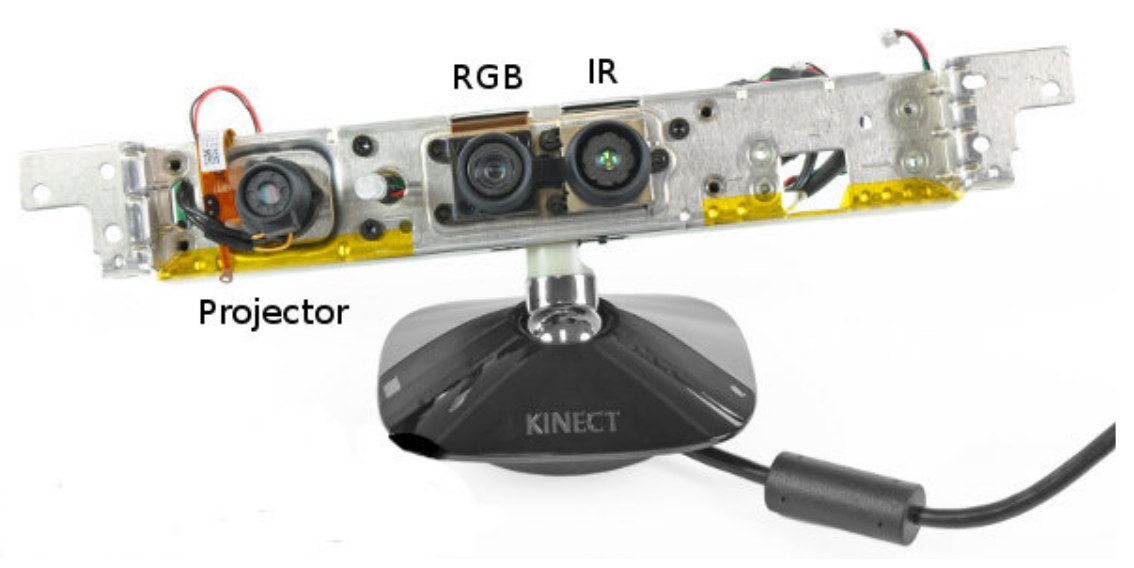
\includegraphics[width=0.65\linewidth,natwidth=640,natheight=640]
	{fig/ref_imgs/kinect_pic.png}
  \caption[Microsoft Kinect V1]{Microsoft Kinect V1 is a RGB-D camera that has 
  640 $\times$ 480 pixels spatial resolution, 0.8-4.0 $m$ depth range, 2-40 
  $mm$ depth resolution and 30 fps \cite{Smisek2011}.}
	\label{fig:kinect_pic}
\end{figure}

While mapping a point from 3D space to 2D space, we lose the 
depth information.  Although there are ways to recover relative depth scale by 
taking images from different poses with a monocular camera, they can't provide 
metric depth.  In this thesis, we are interested in cameras that offer metric 
depth using stereo cameras, more specifically active stereo camera. One can 
model these active stereo cameras with \textit{Triangulation Model}. That 
being said, these two models cannot be used without having the camera to be 
\textit{calibrated} since many anomalies occur in manufacturing.


\section{The Pinhole Model} \label{sc_pinhole}

The light rays are captured through the camera's lens onto an electronic plate 
(called \textit{image plane} in computer vision) that convert light intensity 
to electrical signals.  The pinhole model is, on the other hand, an 
approximation which simplifies this operation.  In this model, the camera 
centre sits behind the image plane.  The Z-axis, so-called \textit{principal 
axis}, of this coordinate system points out through the origin of the image 
plane, and the point where pierce through image plane is called the 
\textit{principal point} $\mathbf{p}$.  We can also see how other two axes; 
i.e., X and Y, are located in figure \ref{fig:pinhole} and this is known as 
the \textit{camera coordinate system}.


\begin{figure}[H]
	\centering
	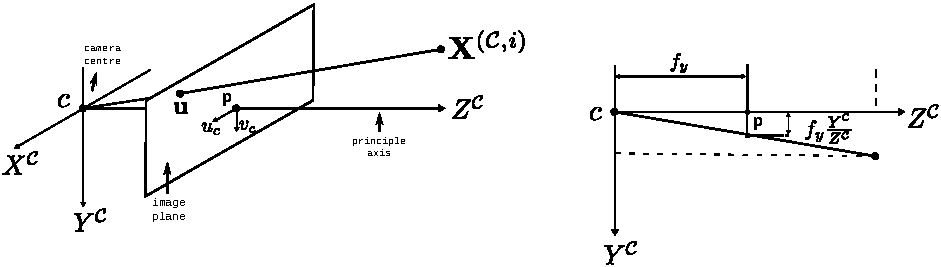
\includegraphics[width=\linewidth,natwidth=640,natheight=640]
  {fig/drawings/pinhole_3d2d.pdf}
  \caption[The Pinhole Model]{In the Pinhole Model, $C$ is the camera centre 
  and $\mathbf{p}$ is the principle point. A 3D point $\mathbf{X_c}$ in the 
  camera coordinate system is projected as a 2D point $\mathbf{u}$ onto the 
  image plane. Note that the camere coordinate system is drawn according to 
  right-hand rule. The illustration is redrawn from \cite{RichardHartley2003} 
  accordingly.}
	\label{fig:pinhole}
\end{figure}

Thanks to geometrical propotion property, we can project the 3D point 
$\mathbf{X_c}=(X_c, Y_c, Z_c)^T$ in the camera coordinate system to the 2D 
point $\mathbf{u} = (f_xX_c/Z_c, f_yY_c/Z_c)^T$ on the image plane, where 
$f_x$ and $f_y$ are the \textit{focal lengths} between the camera centre and 
the pricipal point with respect to horizontal and vertical axis of the camera 
coordinate system respectively.  After projection, we obtain a 2D point  
as \textit{pixel coordinates} $\mathbf{u}=(u,v)^T$ on the image plane.  To 
be more specific, we can write the projection operation as a linear mapping 
function in the following way if we utilize the homogeneous coordinates:

\begin{equation}
  \begin{pmatrix}
    U\\
    V\\
    1
  \end{pmatrix}
  \sim
  Z_{c}
  \begin{pmatrix}
    f_x\frac{X_{c}}{Z_{c}}\\
    f_y\frac{Y_{c}}{Z_{c}}\\
    1
  \end{pmatrix}
  =
  \begin{pmatrix}
    f_xX_{c}\\
    f_yY_{c}\\
    Z_{c}
  \end{pmatrix}
  =
  \begin{bmatrix}
    f_x & 0 & 0 & 0\\
    0 & f_y & 0 & 0\\
    0 & 0 & 1 & 0\\
  \end{bmatrix}
  \begin{pmatrix}
    X_{c}\\
    Y_{c}\\
    Z_{c}\\
    1
  \end{pmatrix}
\end{equation} \label{eq:proj_func_w_f}

This equation applies for the case when 3D points are projected onto a plane 
where the principal point is the origin.  However, the common convention in 
practice is to have the origin at the corner \cite{RichardHartley2003}, 
instead of the centre.

\begin{figure}[H]
	\centering
  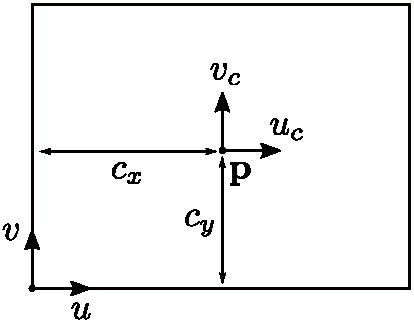
\includegraphics[width=0.4\linewidth,natwidth=640,natheight=640]
  {fig/drawings/pinhole_cam_offset.pdf}
	\caption[Principle Point Offset]{We take OpenCV's pixel coordinate 
	convention where the origin is located at the upper left corner. In order 
	to shift the origin from camera centre to the corner, $c_x, c_y$ principle 
	point offsets are added.}
	\label{fig:pinhole_offset}
\end{figure}

Thus, we get offsets, which can further be added as:

\begin{equation}
  \begin{pmatrix}
    U\\
    V\\
    1
  \end{pmatrix}
  \sim
  Z_c
  \begin{pmatrix}
    \frac{f_x X_c + Z_c c_x}{Z_c}\\
    \frac{f_y Y_c + Z_c c_y}{Z_c}\\
    1
  \end{pmatrix}
  =
  \begin{pmatrix}
    f_xX_c + Z_c c_x\\
    f_yY_c + Z_c c_y\\
    Z_c
  \end{pmatrix}
  =
  \begin{bmatrix}
    f_x & 0 & c_x & 0\\
    0 & f_y & c_y & 0\\
    0 & 0 & 1 & 0\\
  \end{bmatrix}
  \begin{pmatrix}
    X_c\\
    Y_c\\
    Z_c\\
    1
  \end{pmatrix}\label{eq:proj_func_w_f_c}
\end{equation} 

where $c_x$ and $c_y$ are coordinates of the principal point \textbf{p}.
In addition to principal offsets, an inaccurately synchronized pixel-sampling 
process can result in \textit{skewed pixels}. This camera imperfection leads 
to non-square pixels as seen in figure \ref{fig:skewed}.

\begin{figure}[H]
	\centering
  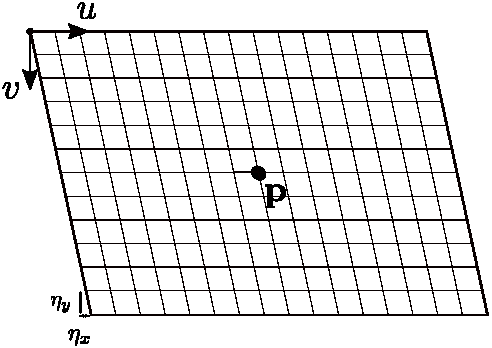
\includegraphics[width=0.4\linewidth,natwidth=640,natheight=640]
  {fig/drawings/pinhole_skew.pdf}
  \caption[Skewed Pixels]{Skewed pixels occur in earlier versions of CCD 
  cameras because the camera's detector array is not orthogonal to the 
  principle axis. This design issue is mostly fixed in modern camera and thus 
  it is usually neglected by taking $\eta_x=1$, $\eta_y=1$ and $s=0$.}
	\label{fig:skewed}
\end{figure}

We can scale the square pixels, having 1:1 pixel aspect ratio, with the 
corresponding skew parameters $\eta_x$, $\eta_y$ and $s$:

\begin{equation} \label{eq:proj_func_w_square_pix_skew}
  \begin{pmatrix}
    U\\
    V\\
    1
  \end{pmatrix}
  \sim
  \begin{bmatrix}
    f_x\eta_x & s & c_x & 0\\
    0 & f_y\eta_y & c_y & 0\\
    0 & 0 & 1 & 0\\
  \end{bmatrix}
  \begin{pmatrix}
    X_c\\
    Y_c\\
    Z_c\\
    1
  \end{pmatrix}
  =
  \begin{bmatrix}
    \alpha_x & s & c_x & 0\\
    0 & \alpha_y & c_y & 0\\
    0 & 0 & 1 & 0\\
  \end{bmatrix}
  \begin{pmatrix}
    X_c\\
    Y_c\\
    Z_c\\
    1
  \end{pmatrix}
\end{equation} 

At this point, we can extract the following matrix:

\begin{equation}
  \mathbf{K_{RGB}} = 
  \begin{bmatrix}
    \alpha_x & s & c_x\\
    0 & \alpha_y & c_y\\
    0 & 0 & 1\\
  \end{bmatrix}\label{eq:k_matrix}
\end{equation} 

where $\mathbf{K_{RGB}}$ is called \textit{intrinsic matrix}, which represents 
the characteristics of a camera sensor.  With this matrix, one can further 
reformulate the notation \ref{eq:proj_func_w_square_pix_skew} in more compact 
form:

\begin{equation}\label{eq:simplyfied_proj_func}
  \mathbf{u} = \mathbf{K_{RGB}}[\mathbf{I}|\mathbf{0}]\mathbf{X_{c}}
\end{equation} 

\begin{figure}[H]
	\centering
  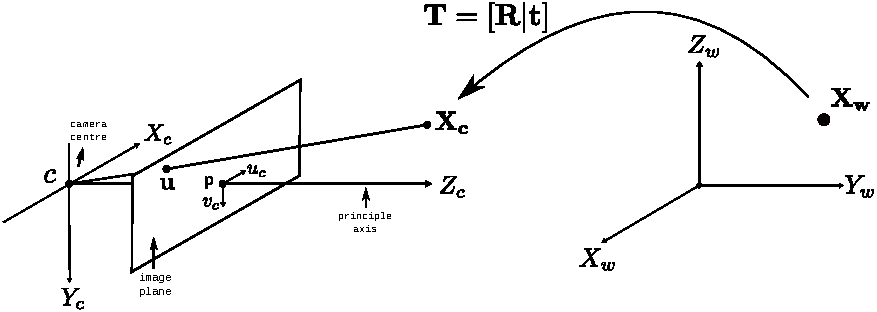
\includegraphics[width=\linewidth,natwidth=640,natheight=640]
  {fig/drawings/pinhole_world_to_cam.pdf}
  \caption[Extrinsic Matrix]{The Z-axis of the camera coordinate system aligns 
  with the principal axis that is \textit{local} to camera frame. In fact, we 
  have measured 3D points that we know their position in the \textit{world 
  coordinate system} which is also refer to the \textit{global frame}, as 
  opposed to the camera coordinate system referring to
\textit{local frame}.}
  \label{fig:cam_model_rot_trans}
\end{figure}

Remember that we measure 3D points in the real-world with respect to the 
camera centre.  Thus, these two coordinates systems, i.e., the camera and 
world coordinate system, can be transformed one another by a rotation and a 
translation as it is depicted in figure \ref{fig:cam_model_rot_trans} and we 
are interested in converting from the world coordinate system to the camera 
coordinate system in the context of projection operation.  To do so, we 
perform series of rotations around each axis of the Cartesian coordinate 
system in $\R^3$ Euclidean space by using \textit{rotation matrices} where 
$R_x, R_y, R_z \in SO(3)$ is the rotation group:

\begin{equation}
  R_x(\alpha) = 
  \begin{bmatrix}
    1 & 0 & 0\\
    0 & cos\alpha & -sin\alpha\\
    0 & sin\alpha & cos\alpha
  \end{bmatrix}\label{eq:rot_matrx_x}
\end{equation} 

\begin{equation}
  R_y(\beta) = 
  \begin{bmatrix}
    cos\beta & 0 & -sin\beta\\
    0 & 1 & 0\\
    sin\beta & 0 & cos\beta
  \end{bmatrix}\label{eq:rot_matrx_y}
\end{equation} 

\begin{equation}
  R_z(\gamma) = 
  \begin{bmatrix}
    cos\gamma & -sin\gamma & 0\\
    sin\gamma & cos\gamma & 0\\
    0 & 0 & 1
  \end{bmatrix}\label{eq:rot_matrx_z}
\end{equation} 

Let's concatenate all three rotations about axes z, y, x respectively (also 
called \textit{yaw, pitch, yaw}) by the matrix multiplication:

\begin{equation}
  \mathbf{R} = \mathbf{R_z(\gamma)}\mathbf{R_y(\beta)}\mathbf{R_x(\alpha)}
  =
  \begin{bmatrix}
    r_{11} & r_{12} & r_{13}\\
    r_{21} & r_{22} & r_{23}\\
    r_{31} & r_{32} & r_{33}\\
  \end{bmatrix}\label{eq:rot_matrix_derivation}
\end{equation} 

Then, we add a translation $\mathbf{t} \in \R^{3x1}$:

\begin{equation}
  \mathbf{t} = 
  \begin{bmatrix}
    t_x \\ t_y \\ t_z
  \end{bmatrix}\label{eq:translation}
\end{equation} 

For convenience, we stack the rotation matrix and the translation vector into 
one:

\begin{equation}
  \mathbf{T_{RGB}} =
  \begin{bmatrix}
    r_{11} & r_{12} & r_{13} & t_x\\
    r_{21} & r_{22} & r_{23} & t_y\\
    r_{31} & r_{32} & r_{33} & t_z\\
  \end{bmatrix}\label{eq:transformation_matrix}
\end{equation} 

The $\mathbf{T_{RGB}} \in \R^{4x3}$ matrix in fact represents a 
\textit{transformation} from 3D position in the world coordinate system to the 
camera coordinate system, which we call \textit{extrinsic camera parameters}.  
Finally, we combine intrinsic $\mathbf{K_{RGB}}$ and extrinsic 
$\mathbf{T_{RGB}}$ matrices in the following form:

\begin{equation}\label{eq:simplyfied_proj_func_1}
  \mathbf{u} = 
  \mathbf{P_{RGB}}\mathbf{X_{w}} = 
  \mathbf{K_{RGB}}\mathbf{T_{RGB}}\mathbf{X_{w}} = 
  \mathbf{K_{RGB}}[\mathbf{R}|\mathbf{t}]\mathbf{X_{w}} =
  \mathbf{K_{RGB}}\mathbf{X_{c}}
\end{equation} 

where $\mathbf{P_{RGB}}$ is the \textit{projection matrix}. All of these 
series of linear operations can be written as a function too:

\begin{equation}\label{eq:simplyfied_proj_func_2}
  \mathbf{u} = \mathbf{F_{p}}(\mathbf{X_{w}})
\end{equation} 

where $\mathbf{F_{p}}(\mathbf{X_{w}})$ is the \textit{projection function}, 
which takes the 3D points in the world coordinate system, transforms to the 
camera coordinate systems and then maps them onto the image plane.

\begin{figure}[H]
\begin{tabular}{ccc}
\centering
\subcaptionbox{Undistorted Image}{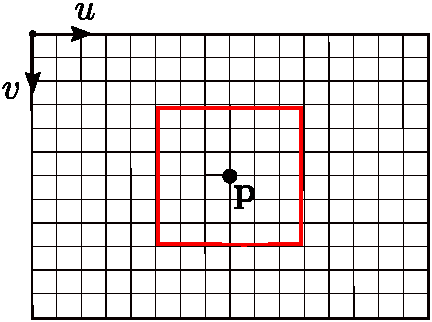
\includegraphics[width = 0.3\linewidth]{fig/drawings/pinhole_undistort.pdf}} &
\subcaptionbox{Barrel Distorted Image}{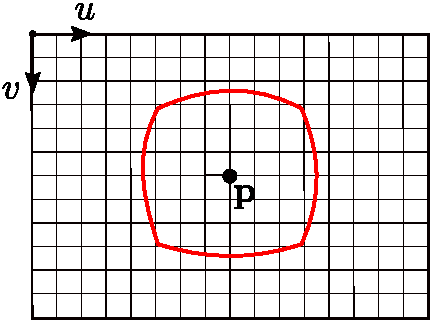
\includegraphics[width = 0.3\linewidth]{fig/drawings/pinhole_distort_1.pdf}}
\subcaptionbox{Pincushion Distorted Image}{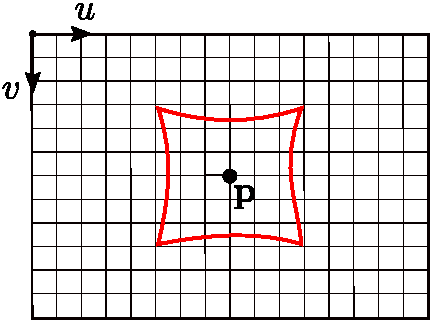
\includegraphics[width = 0.3\linewidth]{fig/drawings/pinhole_distort_2.pdf}}
\end{tabular}
\caption[Radial Distortion]{All emitted 
  lights through the camera lens is expected to intersect at the same 
  focus point and the radial distortion is caused by having a defected lens 
  that causes the emitted lights focusing different points.
  This makes the straight lines appear to be curved.}
\end{figure}\label{fig:}

One last issue with regards to imperfect pixels is the \textit{radial 
distortion}.  The distortion effect has non-linear characteristics. Thus, we 
introduce polynomial function whose coefficients $\kappa = (k_1, k_2, p_1, 
p_2, k_3)^T$ can be fitted by optimization. The polynomial function is given 
as follows:

\begin{equation}
\begin{split}
  x'' = \mathbf{F_{d}}(x') = 
  x'(1+ k_1 r^2 + k_2 r^4 + k_3 r^6) + 2 p_1 x' y' + p_2 (r^2+2x'^2)\\
  y'' = \mathbf{F_{d}}(y') = 
  y'(1+ k_1 r^2 + k_2 r^4 + k_3 r^6) + p_1 (r^2+2y'^2) + 2p_2 x'y'\\
\end{split}
\end{equation}

where $x' = X_{c}/Z_{c}$ and $y' = Y_{c}/Z_{c}$. Now, we can update the 
projection function:

\begin{equation}
  \begin{pmatrix}
    U\\
    V\\
    1
  \end{pmatrix}
  =
  \begin{pmatrix}
    \alpha_x x'' + sy''+ c_x\\
    \alpha_y y'' + c_y\\
    1
  \end{pmatrix}
    =
      \mathbf{K}
      \mathbf{F_{d}}\begin{pmatrix}
      \begin{pmatrix}
        X_{c}/Z_{c}\\
        Y_{c}/Z_{c}\\
        1
      \end{pmatrix}
    \end{pmatrix} 
    =
    \mathbf{K}
    \mathbf{F_{d}}\begin{pmatrix}
       [\mathbf{R}|\mathbf{t}]
      \begin{pmatrix}
        X_{w}\\
        Y_{w}\\
        Z_{w}\\
        1
      \end{pmatrix}
    \end{pmatrix}\label{eq:proj_func_w_f_c}
\end{equation} 

Let's combine projection and distortion function into one:

\begin{equation}\label{eq:simplyfied_dist_proj_func}
  \mathbf{u} = \mathbf{F_{dp}}(\mathbf{X_{w}})
\end{equation} 


To build any reliable computer vision application with digital cameras, it is 
essential to find the parameters of the projection matrix and the radial 
distortion.  The next section describes one of many numerical methods for 
estimating them in literature.

\section{The Triangulation Model} \label{sc_depth_model}

Projected images captured by RGB cameras lack depth and angle information. To 
acquire this information, two main techniques are developed; e.g., passive 
stereo cameras and active stereo cameras. For passive stereo cameras, 
typically two synchronized cameras are placed horizontally with a known 
distance to each other. 
Whereas, for an active stereo camera, one typically has one light projector 
and one camera sensor. For example, in Kinect, an Infrared (IR) laser projects 
structured IR speckle light pattern on an object, and then the deformed light 
due to 3D geometry of the object is captured with a monochrome IR camera from 
a different position.

\begin{figure}[H]
	\centering
  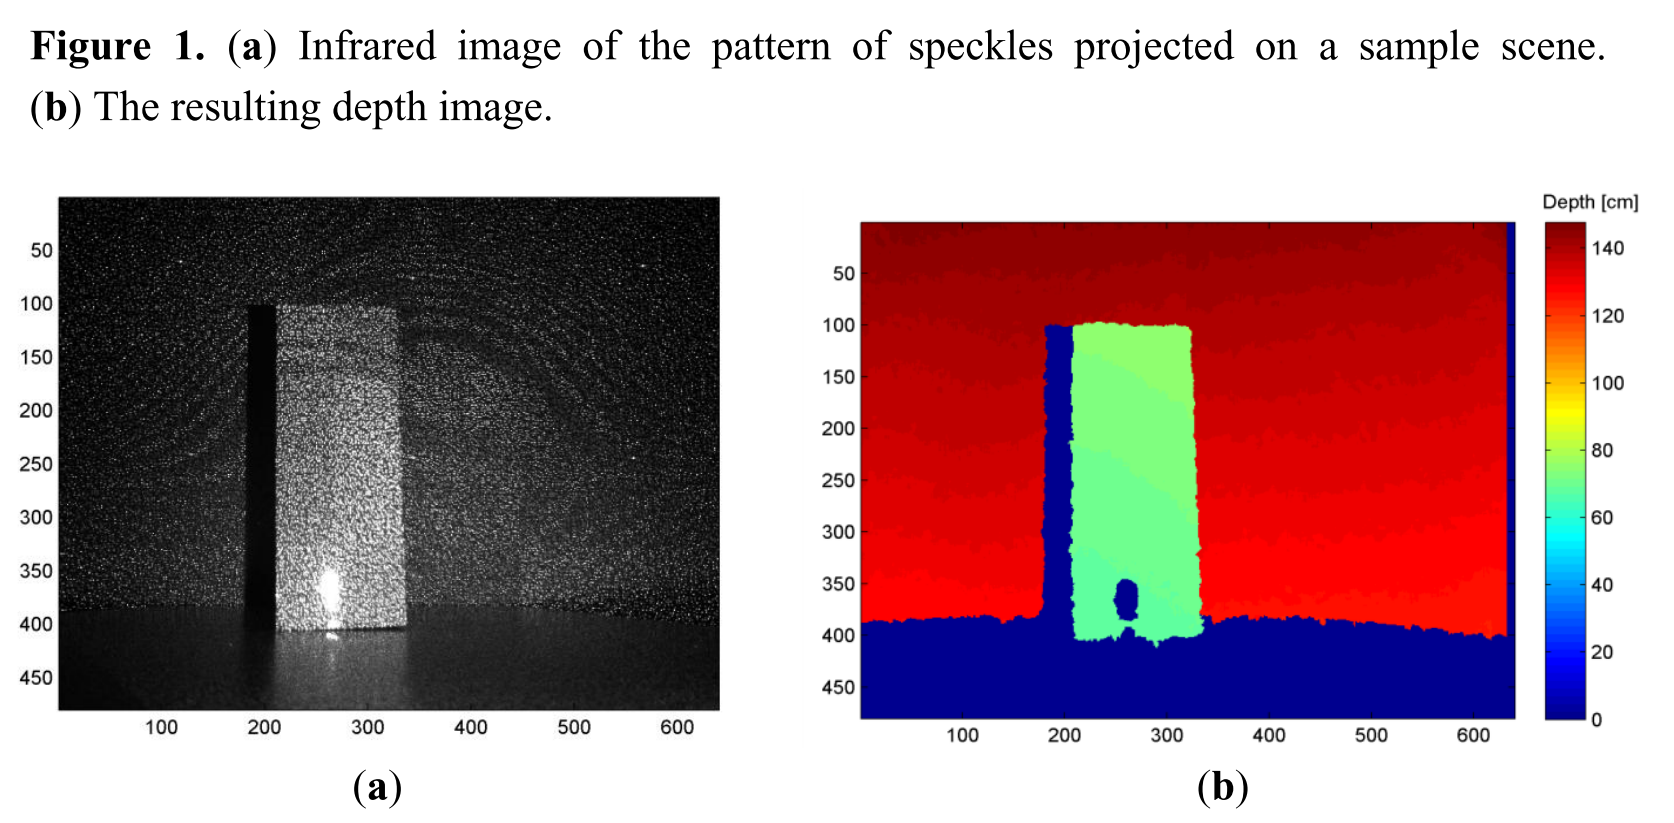
\includegraphics[width=0.7\linewidth,natwidth=640,natheight=640]
  {fig/ref_imgs/kinect_depth_img.png}
  \caption[Kinect's Depth Measurement]{On the left, the IR camera capture the 
  patterns of speckles projected on an object. On the right, we see the 
  resulting depth image if disparity data is converted accordingly 
  \cite{Khoshelham2012a}.}
	\label{fig:kinect_depth_img}
\end{figure}

Since we use Kinect V1 to retrieve depth information for our experiments, we will 
be modeling active stereo vision principle even though the basic principle 
behind them is the same mathematical model, which is the \textit{triangulation 
model}. As shown in figure \ref{fig:triangulation_model}, this model is a 
geometrical model that takes advantages of similarity triangles to calculate 
the depth.

\begin{figure}[H]
	\centering
  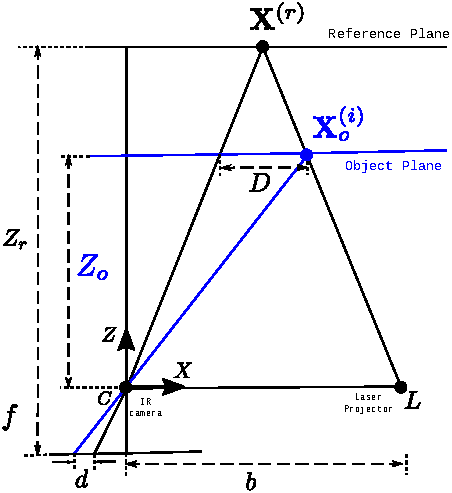
\includegraphics[width=0.65\linewidth,natwidth=640,natheight=640]
  {fig/drawings/triangulation.pdf}
  \caption[The Depth Measurement Model]{The Depth Measurement Model}
	\label{fig:triangulation_model}
\end{figure}

In this setup, we again utilize the camera coordinate system similar to RGB 
camera and IR camera with $f$ focal length is placed by facing perpendicular 
to the (principle axis) Z-axis at the origin. Then, IR laser projector is also 
placed along the X-axis parallel to the IR camera with \textit{baseline} 
$b$ distance.  
Additionally, we measure $d$ as a \textit{disparity} data and the maximum 
range that can be measured refers to $Z_r$. Ultimately, we are interested in 
finding $Z_c$ distance if depth information of point $\mathbf{X_c}^{(i)}$ is 
desired. For doing so, we build two useful relationships using similarity of 
triangles:


\begin{equation}
  \frac{D}{b} = \frac{Z_r - Z_c}{Z_r} \text{ and } \frac{d}{f} = \frac{D}{Z_c}
\end{equation}

If the depth camera parameters such as $f, b,$ and $Z_r$ is calibrated and we 
get $d$ disparity data, we can easily extract $Z_c$ depth information with the 
following formula:

\begin{equation}\label{eq:depth_wo_disparity}
  Z_c = \frac{Z_r}{1+\frac{Z_r}{fb}d}
\end{equation}

Another critical point to note is that Kinect or other depth cameras might not 
provide the depth metric information directly in practice. For instance, 
Kinect provides us disparity image data that correspond to inverse depth 
quantized with 11 bits and the relationship between disparity data and real 
depth is non-linear as shown in figure \ref{fig:depth_disparity_relation}.

\begin{figure}[H]
	\centering
  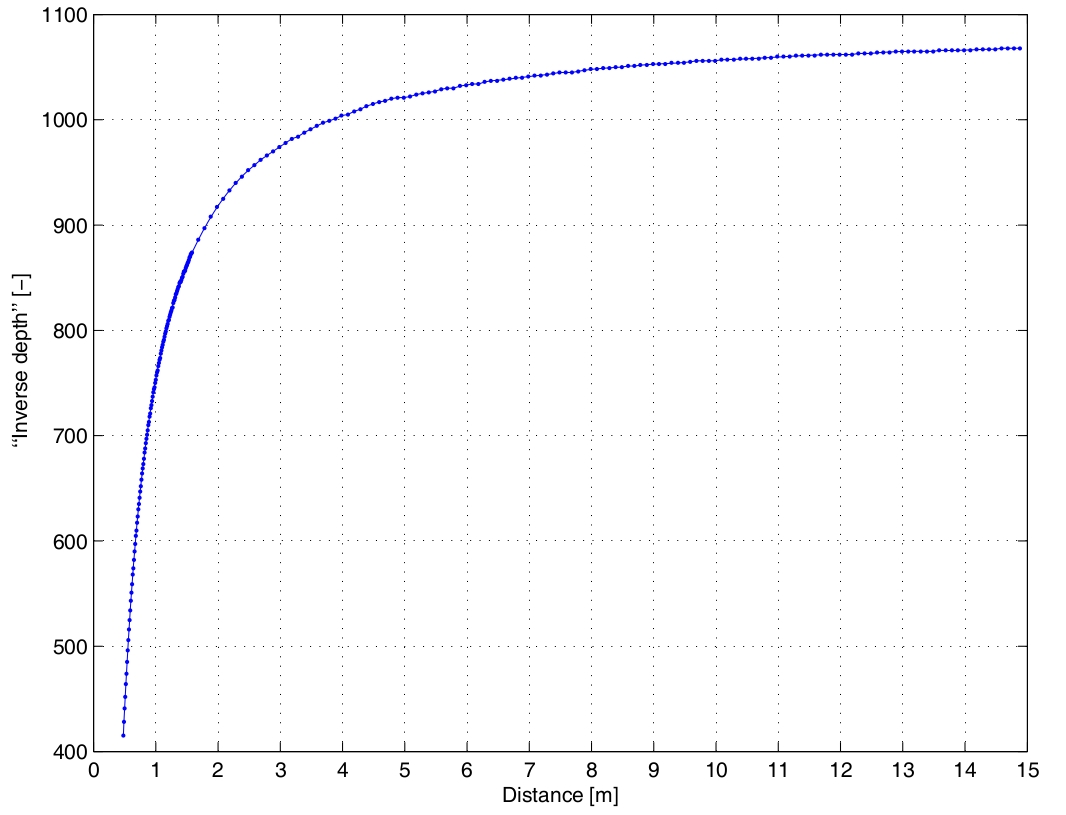
\includegraphics[width=0.6\linewidth,natwidth=640,natheight=640]
  {fig/ref_imgs/depth_disparity_relation.png}
  \caption[Relationship Between Inverse Depth and Disparity]{Non-linear 
  Relationship Between Inverse Depth and Disparity \cite{Smisek2011}}
	\label{fig:depth_disparity_relation}
\end{figure}

Thus, we need to update depth equation \ref{eq:depth_wo_disparity} by taking 
its inverse and introducing normalization factor replacing with $d$ with 
$md'+n$:

\begin{equation}\label{eq:depth_w_disparity_reverse}
  Z_c^{-1} = (\frac{m}{fb})d' + (Z_r^{-1} + \frac{n}{fb})
\end{equation}

To make it convenient to calculate, we can take its inverse again:

\begin{equation}\label{eq:depth_w_disparity}
  Z_c = \frac{1}{(\frac{m}{fb})d' + (Z_r^{-1} + \frac{n}{fb})}
\end{equation}

The relationship between disparity data and metric depth measurement can be 
written as a function in the following form:

\begin{equation}\label{eq:ir_cam_proj_func}
  Z_c
  =
  F_d(d')
\end{equation} 


Now that we know how to get metric depth information $Z_c$ from disparity data 
by utilizing the triangulation model, we can briefly write down similar 
projection operation for the IR camera.

\begin{equation}\label{eq:ir_cam_proj_func}
  \mathbf{u} 
  =
  %Z_i (\mathbf{P_{IR}^{-1}}\mathbf{u}) = 
  \mathbf{K_{IR}} \mathbf{F_d} (\mathbf{T_{IR}}  \mathbf{X_{w}})
\end{equation} 


Keep in mind that we first need to calibrate the IR camera's intrinsic and 
extrinsic paratemeters to find related depth related parameters, i.e., 
$f,b,Z_r,m, n$. In the following section, we will discuss how calibration 
processes are performed for RGB-D camera to measure quality data.

\section{RGB-D Camera Calibration} \label{sb_sc_rgb_calibration}

The calibration process is a crucial part of any computer vision applications, 
and there are many sophisticated techniques to achieve accurately.  However, 
it is important to note that full derivations of the calibration formulation 
are not provided in this thesis, but only the important points are given.  
Therefore, I refer readers to \cite{Zhang2000a}, \cite{Smisek2011}, 
\cite{Karan2015} and \cite{Herrera2016a} for the details of a RGB-D camera 
calibration.  Since we are about to perform 3 calibration operation: RGB 
camera, IR camera, and depth measurement, we assume that both RGB and IR 
camera's image planes are aligned for simplicity (in practice, one must 
  perform transformation $\mathbf{T}_{RGB,IR}$ between RGB 
and IR camera if a feature from RGB camera used in IR camera) and they have 
1:1 pixel correspondences. Under these assumptions, let's start with RGB and 
IR camera.

\subsubsection{RGB and IR Camera Calibration}

We calibrate RGB and IR camera since they both project 3D space to 2D space, 
but only measuring the different light spectrum. Thus, the calibration process 
for the RGB camera that we will discuss applies for the IR Camera as well.  To 
begin with, the simplest case which can help us to understand the calibration 
process is that we assume that we know the exact position of 3D points in 
world coordinate system and exact position of 2D points on the image plane.  
One can build a constraint between them by exploiting the projection function:

\begin{equation}
  \mathbf{u_{RGB}}^{(i)} = 
  \begin{pmatrix}
    u^{(i)}\\
    v^{(i)}\\
    1
  \end{pmatrix}
  =
  \mathbf{P_{RGB}}\mathbf{X_{w}} = 
  \begin{bmatrix}
    p_{00} & p_{01} & p_{02} & p_{03}\\
    p_{10} & p_{11} & p_{12} & p_{13}\\
    p_{20} & p_{21} & p_{22} & p_{23}
  \end{bmatrix}
  \begin{pmatrix}
    X^{(i)}_w\\
    Y^{(i)}_w\\
    Z^{(i)}_w\\
  \end{pmatrix}\label{eq:proj_matrix}
\end{equation} 

Let's now distribute the projection matrix onto the 3D point measurement to 
retrieve individual pixel coordinates:

\begin{equation}\label{eq:u_i}
  u^{(i)} = 
  \frac
  {p_{00}X^{(i)}_w + p_{01}Y^{(i)}_w + p_{02}Z^{(i)}_w + p_{03}}
  {p_{20}X^{(i)}_w + p_{21}Y^{(i)}_w + p_{22}Z^{(i)}_w + p_{23}}
\end{equation} 

\begin{equation}\label{eq:v_i}
  v^{(i)} = 
  \frac
  {p_{10}X^{(i)}_w + p_{11}Y^{(i)}_w + p_{12}Z^{(i)}_w + p_{13}}
  {p_{20}X^{(i)}_w + p_{21}Y^{(i)}_w + p_{22}Z^{(i)}_w + p_{23}}
\end{equation} 


Since $\mathbf{u}$ and $\mathbf{X_{w}}$ are known, we can find elements of the 
$\mathbf{p} = (p_{00}, p_{01}, \dots, p_{23})^T$ matrix by solving 
$\mathbf{Ap=0}$ liner system of equations from \ref{eq:u_i} and \ref{eq:v_i}.  
For \textit{minimal solution} of this linear system of equations, we need at 
least $n \geq 6$ measurement points to solve the problem as the 
$\mathbf{P_{RGB}}$ matrix has 12 unknowns (11 if scale is ignored).  Note that 
this accounts for having noise-free measurement which does not hold in 
reality. Then, the problem becomes \textit{over-determined}.

\begin{figure}[H]
%\begin{tabular}{cc}
\centering
\subcaptionbox{RGB Images}{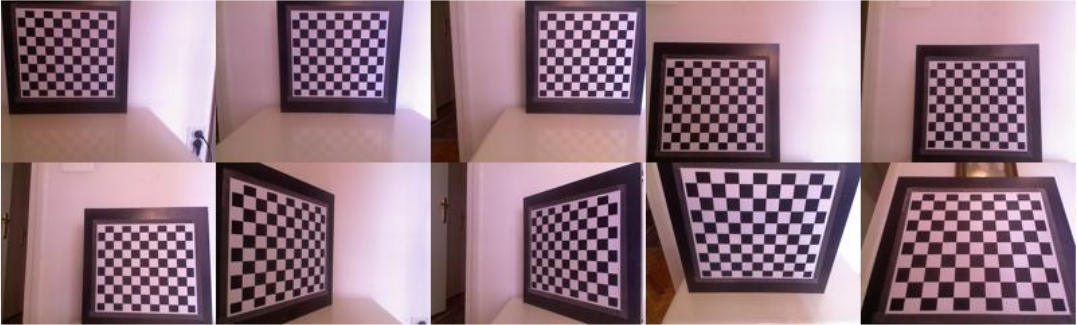
\includegraphics[width = 0.8\linewidth]{fig/ref_imgs/checkerboard_rgb.png}} \\
\subcaptionbox{IR Images}{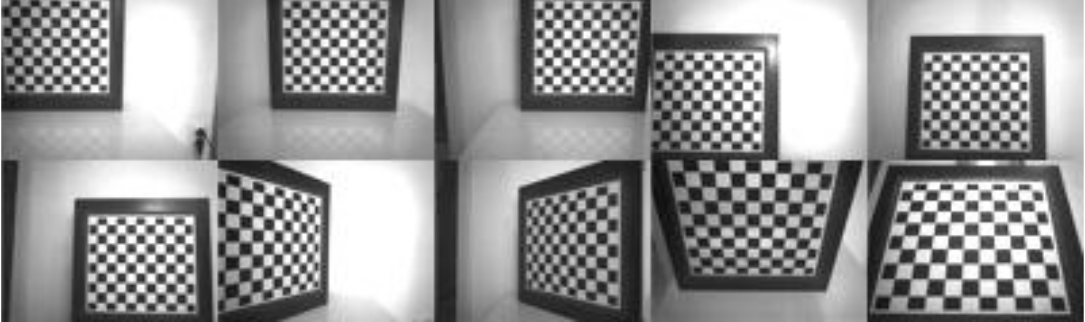
\includegraphics[width = 0.8\linewidth]{fig/ref_imgs/checkerboard_ir.png}}
%\end{tabular}
\caption[Checkboard Calibration for RGB and IR Camera]{When calibrating RGB 
and IR camera with a checkerboard, one should produce many measurement points 
by placing checker board at different orientation and different tilted 
posture \cite{Karan2015}.}
\end{figure}\label{fig:}


In noisy measurement case, the problem is usually solved with \textit{singular 
value decomposition (SVD)} with $n > 6$ measurement points.  This method is 
called the \textit{Direct Linear Transformation (DLT)}.  Disadvantage of the 
DLT methods, it is still sensitive errors since it only considers algebraic 
errors (that are the residuals of $\mathbf{Ap}$).  Another drawback of DLT is 
that it cannot compensate non-linearities of projection function due to the 
radial distortions.  Thus, instead of DLT, the non-linear least squares 
optimization is usually performed for the better accuracy:

In practice, the checkerboard is used to get many good measurement points as 
we can easily extract edge features from the image as 2D points.  Plus, we 
also know the corresponding 3D positions in the world coordinate system.
Also, we have prior knowledge about some of the parameters of intrinsic 
matrix, e.g., pixels are squared, skew factor is trivial, optical center near 
the center of the image. All of these can increase our chance for successful 
convergence when optimizing:

\begin{equation}\label{eq:proj_lsq}
  \argmin_{\mathbf{F_{dp}} \rightarrow \mathbf{K_{RGB}}, \kappa_{RGB}, \mathbf{R_{RGB}}^{(i)}, \mathbf{t_{RGB}}^{(i)}}
  \sum_{i=1:n} || \mathbf{u_{RGB}}^{(i)} - 
  \mathbf{F_{dp}} (\mathbf{X_w}^{(i)}) ||^2
\end{equation}

where $\mathbf{F_{dp}}$ is the projection function along with distortion (see 
notation \ref{eq:simplyfied_dist_proj_func}), $\mathbf{u}_{(i)}$ is the 
measured pixel coordinates of a feature on image plane and 
$\mathbf{X_w}_{(i)}i$ is the 3D coordinates of a feature in world coordinate 
system to identify the following parameters:

\begin{itemize}
  \item $\mathbf{K_{RGB}}$ is the intrinsic matrix for RGB camera, 
  \item $\kappa_{RGB}$ is the distortion coefficients for RGB camera, 
  \item $\mathbf{R_{RGB}}^{(i)}$ is the corresponding orientation for RGB camera and 
  \item $\mathbf{t_{RGB}}^{(i)}$ is the corresponding translation for RGB camera.
\end{itemize}

As mentioned earlier, we can apply the same optimization process for IR camera 
to find $\mathbf{K_{IR}}$ intrinsic matrix for IR camera, $\kappa_{IR}$ 
distortion coefficients for IR camera, $\mathbf{R_{IR}}^{(i)}$ corresponding 
orientation for IR camera and $\mathbf{t_{IR}}^{(i)}$ corresponding 
translation for IR camera.


\subsubsection{Depth Measurement Calibration}

As we discussed in the previous section, disparity data for every pixel on IR 
image corresponds to the metric depth information.  We can only build the 
relationship between pixel coordinates of the IR image and disparity value 
when the IR camera is calibrated and its $\mathbf{u_{IR}}$ pixel measurements 
are corrected accordingly.

\begin{figure}[H]
	\centering
  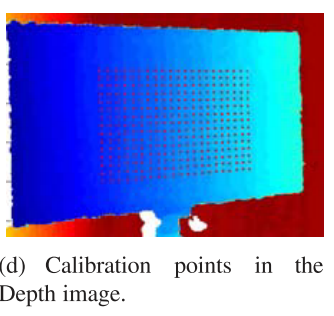
\includegraphics[width=0.7\linewidth,natwidth=640,natheight=640]
  {fig/ref_imgs/checkerboard_depth.png}
  \caption[Checkboard Calibration for Depth]{When calibrating the depth 
  parameters, checkerboard should be placed at the different distances to the 
  camera so that we get enough measurement points, especially for fitting 
  $m,n$ parameters \cite{Karan2015}.}
  \label{fig:checkerboard_depth}
\end{figure}

To get the disparity for $i^{th}$ feature point, a simple mask function can be 
used:

\begin{equation}
  d'^{(i)} = M(\mathbf{u_{IR}}^{(i)})
\end{equation}

where $M$ is a function that return the disparity value at pixel coordinates 
$\mathbf{u_{IR}}^{(i)}=[u_{IR}^{(i)},u_{IR}^{(i)}]^T$ of calibrated IR image.  
Then, our one last step will be to convert disparity measurement to depth for 
every feature on the checkboard and minimize the error between measured depth 
$\hat{Z_c}=F_d(d')$ (see notation \ref{eq:ir_cam_proj_func}) and real depth 
$Z_c$:

\begin{equation}\label{eq:proj_lsq}
  \argmin_{F_d \rightarrow f, b, Z_r, m, n}
  \sum_{i=1:n} || Z_{c}^{(i)} - F_d(d'^{(i)})  ||^2
\end{equation}

The calibration processes for cameras are a well-studied problem in computer 
vision literature.  Fortunately, there are many open software libraries, such 
as OpenCV, that offers such implementations.


\chapter{Fundamentals of Visual Odometry} \label{cp_vo}

\section{Related Work} \label{sc_visual_odometry_related_works}

% First ego motion estimation with cam
% - Moravec1980 - Obstacle Avoidance and Navigatio n in the Real World by a Seeing Robot Rover
% - Matthies1987a - Error Modeling in Stereo Navigation
% - Olson2003 - Rover navigation using stereo ego-motion
First research in estimating camera ego-motion was done in a Ph.D. Thesis 
\cite{Moravec1980} in the 1980s. He used a sliding camera as a stereo fashion 
that captures images when the robot stopped after moving for some small 
distance. Another early study, from Matthies and Shafer \cite{Matthies1987a}, 
formulated the ego-motion estimation for stereo vision. The interest in VO 
peaked after NASA's Mars expeditions with a rover in 2003. Researchers and 
engineers in NASA JPL further improved the robustness of their mobile robots 
with the VO system \cite{Olson2003}.
% First VO Paper
% Nister2004 - Visual Odometry

In computer vision, Structure from Motion (SFM), that tackles 3D 
reconstruction of an environment with moving camera, is a well-studied topic. 
For SFM, it is critical to estimate camera pose accurately to build the 3D 
environment. VO can be thought of subset problem of SFM. The reason VO parted 
from SFM is that VO systems started to empower other applications such SLAM 
and are required to operate in real-time, all of which introduces a great 
challenge.

% Surveys
% - Fraundorfer2012 - Visual odometry: Part I: The First 30 Years and 
%Fundamentals
% - Scaramuzza2011 - Visual Odometry Part II: Matching,Robustness, 
%Optimization, and Applications
% - Aqel2016 - Review of visual odometry: types, approaches, challenges, and 
%applications
For the first time, Visual Odometry term was introduced in \cite{Nister2004}. 
It estimates the transformation matrix by solving the P3P problem between 
consecutive frames. Nister also demonstrated a VO pipeline that became a 
defacto system configuration even for today's VO applications. With the help 
of early robotics applications in NASA and computer vision community, the VO 
became a quite popular field. That being said, two of the most influential 
papers were \cite{Fraundorfer2012} and \cite{Scaramuzza2011}. By publishing 
these tutorials, the authors gave researchers and engineers a design recipe 
for building the VO system for different kind of environment settings since 
there is no such a system that works under any conditions. One can also find a 
survey of VO types, approaches and challenges in \cite{Aqel2016}.

Over the years, research on VO is progressively increased and various types of 
VO systems are proposed. Therefore, VO systems can be categorized based on 
different phenomena such as camera sensor types and solver algorithms choice. 
One can utilize monocular or stereo cameras to capture images. The stereo 
cameras are further grouped into two categories; i.e., active and passive 
cameras. For the active camera, besides color or monochrome camera, there is 
another camera such IR camera that measures the depth information combination 
with IR laser projector. For the passive camera, the depth is calculated from 
two color or a monochrome camera. In the case of solver algorithms, one can 
group VO into two categories; i.e., feature-based and appearance-based.

The feature-based VO algorithms are interested in extracting distinct and 
repeatable feature points from images and finding correspondences in extracted 
features either between consecutive frames or keyframes. The challenging part 
in feature-based VO is to build a system that can match features across 
different frames without errors. However, this does not hold in reality, so 
one typically needs to remove these errors with outlier rejection algorithms 
such as RANSAC \cite{Fischler1981b}. Among many VO systems, there are two 
favorite open source feature-based VO tools which stand out; i.e., LIBVISO2 
\cite{Geiger2011} and FOVIS \cite{Huanga2011}. Briefly, LIBVISO2 uses both 
simple blob and corner filters to extract features. The extracted features are 
filtered by non-maximum suppression to increase the robustness of the matching 
process. Then, it calculates the depth information by triangulation technique 
as it uses a passive stereo camera. Finally, it minimizes the reprojection 
error. The reprojection error function is constructed by projection from 
features on the left camera onto the right camera and vice-versa, to estimate 
the pose. Note that RANSAC applied on feature matches to remove outliers. 
Whereas, FOVIS is more accurate and faster than LIBVISO2 according to 
\cite{Fang2015a}.
% RGBD VO Comparisons
%% - Angladon2017 - An evaluation of real-time RGB-D visual odometry algorithms on mobile devices
% - Fang2015a - Experimental evaluation of RGB-D visual odometry methods
FOVIS uses only FAST corner detectors to extract features. For matching 
features, FOVIS take advantage of keyframes instead of consecutive images to 
reduce the drift. Instead of using RANSAC for outlier rejection, it constructs 
a graph of consistent feature matches and updates the features that obey the 
idea that the Euclidean distance between two features at one time should match 
their distance at another time. Finally, several refinement processes are 
applied during motion estimation to improve accuracy.
% RGBD VO Implementations
% - Geiger2011 - LIBVISO2 - StereoScan: Dense 3d Reconstruction in Real-time
% - Huanga2011 - FOVIS - Visual Odometry and Mapping for Autonomous Flight Using an RGB-D Camera

The most significant disadvantage of feature-based VO is that the accuracy of 
the pose estimations decreases if the operating environment lacks texture-rich 
scenes such as corridors or the measured images are blurry due to fast 
motions. Thus, appearance-based VO algorithms utilize the entire image instead 
of extracted features. Initially, Iterative Closest Point (ICP) 
\cite{Besl1992} was used to minimize the geometrical error between 3D 
surfaces. Then, various kinds of ICP algorithms are built for improving 
efficiency \cite{Rusinkiewicz2001}. Even though ICP is useful for creating 3D 
shapes with point clouds, it is slower and less accurate compared to 
feature-based methods.
% - Besl1992 - First ICP Paper - A method for registration of 3-D shapes
% - Rusinkiewicz2001 - ICP - Efficient Variants of the ICP Algorithm
Then, another type of appearance-based approach, so-called Dense Visual 
Odometry (DVO) \cite{Kerl2013a}, was emerged by minimizing the photometrical 
error based on the pixel intensity between consecutive frames. Although the 
original techniques developed with appearance-based approaches produces less 
accurate results, we can say that it recently started to gain popularity with 
carefully designed hybrid methods, so-called Semi-Dense VO \cite{Zhou2017a}, 
and it can outperform feature-based VO in some cases.
% - Kerl2013a - DVO - Robust Odometry Estimation for RGB-D Cameras

In this chapter, we will focus on the standardized feature-based VO pipeline, 
which will serve us as a foundational basis so that we comprehend the 
algorithmic errors. Hence, We structured this chapter according to four main 
components of the pipeline: (1) feature extraction, (2) feature matching, (3) 
outlier rejection and (4) pose estimation. 

\section{Feature Extraction} \label{sc_feature_extraction}

Image features are a collection of regions of interest or points of interest 
that describe the image. In this way, we compress the necessary information 
from images so that we can deal with computationally expensive image 
processing tasks.  Points of interest, which also can be called as 
\textit{keypoints}, \textit{features} or \textit{landmarks} interchangeably, 
are particularly valuable because their location in the image can be measured 
accurately. This is useful for localization-related tasks such as VO. 

In feature-based VO, the critical task is to find good features.  What defines 
good features from others is that they are distinct, repeatable, 
computationally cheap and invariant to geometrical changes.  One has many 
options to produce such image , but two common methods in VO systems are blobs 
and corners.  Blobs are image patterns that contain distinct image response 
comparing to their neighborhood pixels. Blobs take advantage of pixel 
intensity or color to decide whether it has a distinct response or not.  In 
the VO literature, SIFT \cite{Lowe2004} and SURF \cite{Bay2008} are popular 
choices for detecting blob features.  In contrast, corners are the meeting 
points where two or many edges intersect.  Corners take advantage of the 
geometrical structure of an image.  FAST \cite{Rosten2006} and Harris 
\cite{Harris1988} are widely used for detecting corners.

Fundamentally, a two-step process is needed to extract good features.  First, 
you take a response function called \textit{image filter}, shift this filter 
through the image and save the one that has greater response than your 
previously defined threshold.  This might be a Gaussian filter for blobs or a 
corner detector filter for corners. In the second step, you perform non-maxima 
suppression on the resulting image features to find local minima of the 
function.  This step will help to remove similar image features and to choose 
the ones having maximum confidence so that distinctiveness of the features are 
ensured.  Some VO might skip non-maxima suppression because of the efficiency 
reasons.

Inherently, each feature detector has certain limitations, and one has to 
choose which detector to use depending on task objectives. Therefore, we may 
ask the following question: Does the localization environment involve more 
texture-oriented objects like floors, walls, etc. or geometrical shapes like 
urban areas where many lines exist?  However, the rule of thumb is that blobs 
are distinct but slow to compute and corners are fast to compute but less 
distinct. 

%\subsection{Feature Descriptor} \label{sb_sc_feature_descriptor}

After extracting features, one needs to encode the detected image features 
into a format that we can perform comparison or search operation among them. 
This is done by taking the neighboring pixels around the image features and 
convert into a more compact form. For example, SIFT, most well-known feature 
descriptor, creates a patch around an image feature, divides this patch into 
smaller grids, calculate the gradient of each grid and saves them as a 
histogram.  This procedure makes feature descriptor robust against scale or 
rotation changes. Then, one can use these descriptors for various comparison 
operations such as matching or tracking in VO. However, we utilize the ORB 
that combines feature extraction and description process in our VO.s


\subsubsection{ORB} \label{sb_sc_orb}

One of the most strict requirements of VO is the real-time constraints since 
it is expected to work at similar to low-level inertial sensors, i.e., 
accelerometer, gyroscopes, etc.  As previously discussed, blobs detectors are 
computationally expensive. Therefore, corner-based feature detectors are more 
prevalent in VO.  \textit{ORB} \cite{Rublee2011a} combines FAST detector 
\cite{Rosten2006} and BRIEF descriptor \cite{M.2010} by tuning the necessary 
parameters to produce robust and reproducible features.  In the end, it mostly 
performs as accurate as SIFT, plus faster. Here are steps on how to extract 
features and create descriptors with ORB: 

\begin{enumerate}
  \item \textbf{Detect corners with FAST}: FAST take each pixel on 
    the image and compare with its adjacent pixels. More specifically, 
    ORB uses FAST-9, which takes a patch of a discrete circular radius of 
    $r=9$. 
    \begin{figure}[H]
	\centering
	  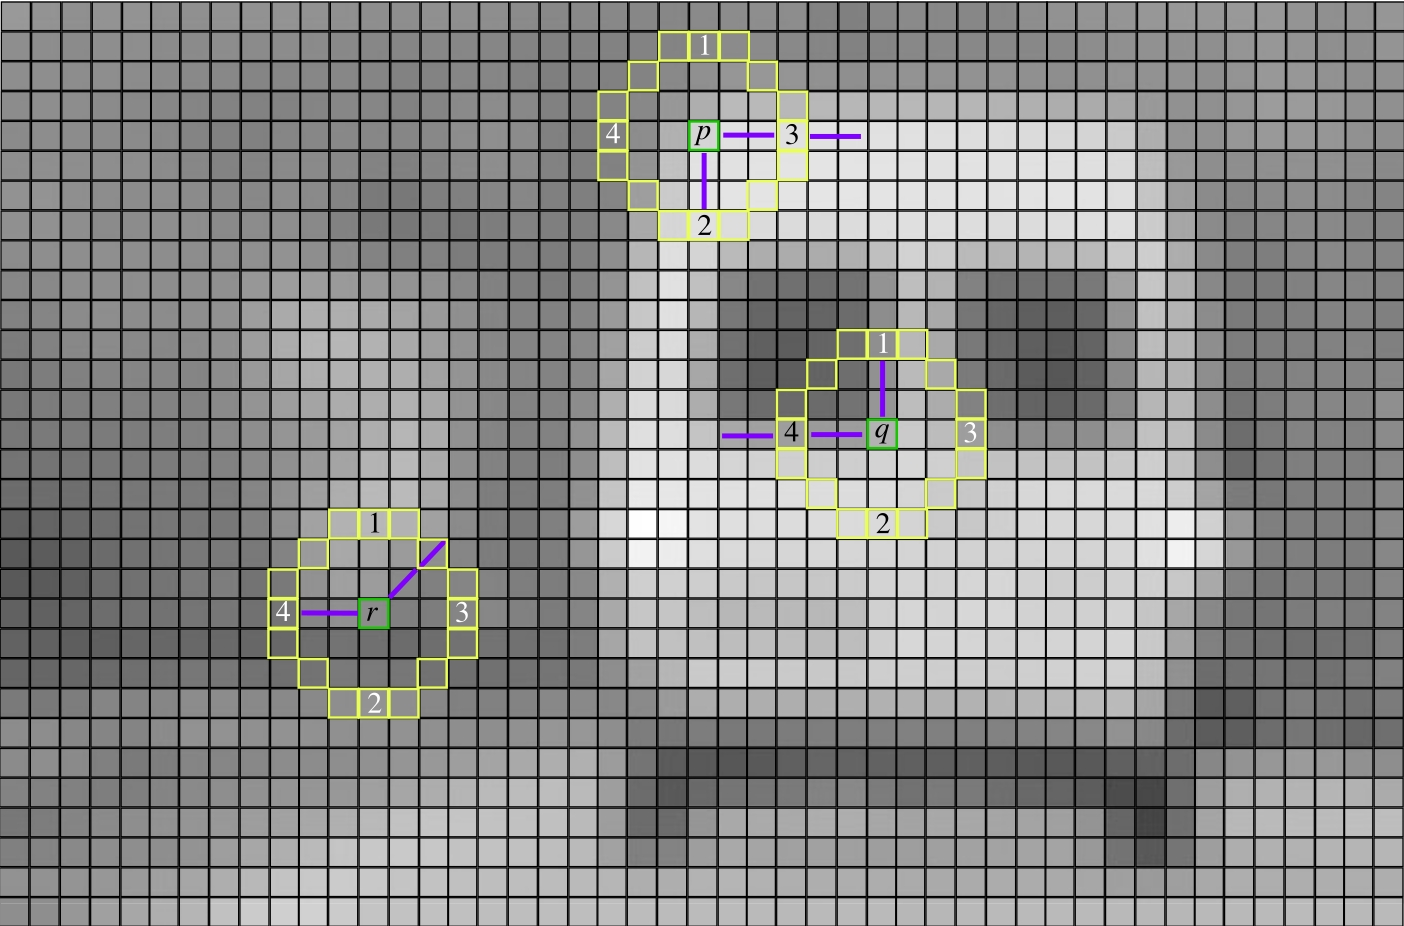
\includegraphics[width=0.7\linewidth,natwidth=640,natheight=640]
	  {fig/ref_imgs/fast.png}
	\caption[FAST Corners]
		{Point of interest or feature points are at the intersection of edges 
		as seen for the $p,q$ and $r$ pixels and the blue lines correspond to 
		the directions of the edges.For this figure, $r=4$ is taken 
		\cite{Klette2014}.}
	  \label{fig:fast_corners}
	\end{figure}

    The basic principle behind FAST is if the selected pixel $p$ is $\pm t$ 
    darker or brighter than adjacent pixels $r\in{1,2,\dots,n}$, we call it a 
    corner, where $t$ is our empiric threshold. Comparison pixel set $r$ is 
    chosen as a circle around in figure \ref{fig:fast_corners}.

    \begin{equation}
      S_{p \rightarrow r} = 
      \begin{cases}
        S_b, & I_{p \rightarrow r} \leq I_p - t \\
        S_d, & I_p - t \leq I_{p \rightarrow r} \\
        S_s, & otherwise
      \end{cases}
    \end{equation}

    If a set of N contiguous pixels are either dark $S_d$ or bright $S_b$, we 
    call interest point $p$ as a corner $\mathbf{u_c} = M_c(p)$, where $M_c$ 
    is a function that returns the pixel coordinates of the corner pixel and N 
    is another empiric parameter whose purpose is to ensure majority of the 
    comparison either dark or bright.For more details about efficient ways to 
    calculate FAST corners, I refer readers to \cite{Rosten2006}.

	\item \textbf{Rank FAST corners with Harris}: After FAST detection, we 
	might get many corner candidates around the interest point. However, FAST 
	does not measure how good a corner is. Thus, we use Harris detector to 
	rank corner candidates:
  
    \begin{equation}
      \mathbf{A} = \sum_{x,y} w(x,y) 
      \begin{bmatrix}
        I_x^2 & I_xI_y \\ I_xI_y & I_y^2
      \end{bmatrix}
    \end{equation}
    
    The $\mathbf{A}$ matrix is calculated by the $I_x$ and $I_y$ partial 
    derivatives with respect to $x$ and $y$ direction on the image plane and 
    $w(x,y)$ weighting window.

    \begin{equation}
      R_c(\mathbf{A}) = det(\mathbf{A}) - k(trace(\mathbf{A}))^2
    \end{equation}
    
    where $det(\mathbf{A}) = \lambda_1 \lambda_2$, $trace(\mathbf{A}) = 
    \lambda_1 + \lambda_2$ and $k$ is an empiric tuning parameter. Then, we 
    use the resulting $\mathbf{A}$ to find a ranking score for each corner. 
    Now, it is possible to take top N corners from if desired.

	\item \textbf{Calculate orientation of corners with image moments}: ORB 
	uses BRIEF to create feature descriptors, but BRIEF fails in rotated 
	images. Therefore, ORB modifies the BRIEF by adding orientation 
	information. To get orientation, an \textit{image moment} are calculated 
	for each patch $\mathbf{S}^{(n)}$:

    \begin{equation}
    m_{a,b}(\mathbf{S}^{(n)}) = \sum_{x,y \in \mathbf{S}^{(n)}} x^a y^b I(x,y)
    \end{equation}
    
    where $a + b$ defines the order of the moment of $n^{th}$ patch and 
    $I(x,y)$ is the intensity of the pixel at the corner. Next, we calculate 
    the moments of order one: 

    \begin{equation}
      m_{1,0}(\mathbf{S}^{(n)}) = \sum_{x,y \in \mathbf{S}^{(n)}} x \cdot I(x,y) \text{  ,  }
      m_{0,1}(\mathbf{S}^{(n)}) = \sum_{x,y \in \mathbf{S}^{(n)}} y \cdot I(x,y)
    \end{equation}

    Then, we get the orientation of the patch $\mathbf{S}^{(n)}$:
    
    \begin{equation}
      \theta(\mathbf{S}^{(n)}) = atan2(m_{0,1}, m_{1,0})
    \end{equation}

	\item \textbf{Form BRIEF descriptors with their corresponding 
	orientation}: Once the top N corners and their orientations are detected, 
	descriptions can be formed with BRIEF. 

	\begin{figure}[H]
		\centering
	  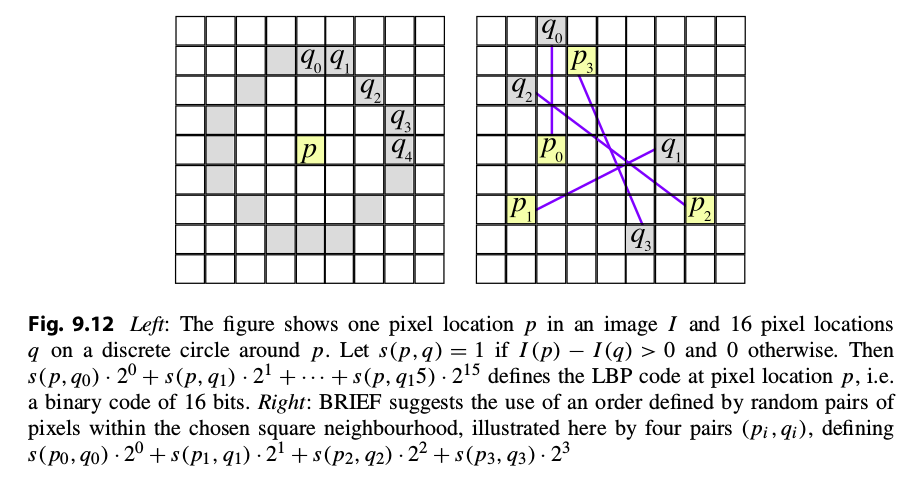
\includegraphics[width=0.6\linewidth,natwidth=640,natheight=640]
	  {fig/ref_imgs/brief.png}
	  \caption[BRIEF Descriptor]{In order to form BRIEF descriptor, one needs 
	  to create group of pixel pairs from patch $\mathbf{S}^{(n)}$. There are 
	  two common ways to create pair. As seen in the left figure, we take the 
	  feature point and pair with pixels around the circle patch. In the right 
	  figure, another method where we pair randomly selected pixels can be 
	  seen. ORB prefers the method on the right \cite{Klette2014}.}
	  \label{fig:brief}
	\end{figure}


    To do so, we randomly (normal distribution) selected 256 pairs 
    $(p^{(i)}=(u^{(i)},v^{(i)},q^{(j)}=(u^{(j)},v^{(j)}))$ inside the patch 
    $\mathbf{S}^{(n)}$:
    
    \begin{equation}
    \mathbf{S}^{(n)} = 
      \begin{pmatrix}
        p^{(0)}, \dots, p^{(255)}\\
        q^{(0)}, \dots, q^{(255)}
      \end{pmatrix}
    \end{equation}
    
	Next, we rotate each $(\mathbf{p}^{(0:255)}, \mathbf{q}^{(0:255)})$ pair 
	points in $\mathbf{S}^{(n)}$ with the corresponding corner's orientation:
	
    \begin{equation}
      \mathbf{p}^{(i)}_{\theta} = \mathbf{R}_{\theta}\mathbf{p}^{(i)} \text{ and } 
      \mathbf{q}^{(j)}_{\theta} = \mathbf{R}_{\theta}\mathbf{q}^{(j)}
    \end{equation}
    
    It is important to note that the authors in \cite{Rublee2011a} suggested 
    to rotate each point in increments of 2$\pi$/30. Therefore, orientation 
    $\theta$ is mapped to nearest multiple of 2$\pi$/30. To form steered (or 
    rotated) BRIEF descriptors, we compare pixel densities of pair points that 
    are selected randomly:
    
    \begin{equation*}
      \tau(\mathbf{p}^{(i)}_{\theta},\mathbf{q}^{(j)}_{\theta}) := 
      \begin{cases}
        1  & I(\mathbf{p}^{(i)}_{\theta} < I(\mathbf{q}^{(j)}_{\theta}),\\
        0  & I(\mathbf{p}^{(i)}_{\theta} \geq I(\mathbf{q}^{(j)}_{\theta})
      \end{cases}
    \end{equation*}

    Finally, we sum comparison results with binary form to get the descriptor  
    of the patch $\mathbf{S}^{(n)}$:
    
    \begin{equation}
      \mathbf{D}^{(n)} = f(\mathbf{S}^{(n)}) := \sum_{0\leq i,j \leq 255} 2^{i-1}\tau (\mathbf{p}^{(i)}_{\theta},\mathbf{q}^{(j)}_{\theta})
    \end{equation}

\end{enumerate}





\section{Feature Matching} \label{sc_feature_matching}

Now that we know how to extract a distinct feature and to form a descriptor, 
we can start building a relationship across images to estimate how the camera 
moves. Remember that the camera can procedure a video stream consisting of 
usually ranging from 30 to 60 frames per second. The second task in VO after 
extracting features is to form a group of image pairs information between each 
image pair, continuously. In literature, there are two ways to select image 
pairs: frame to frame or keyframe to frame. In the former case, one groups 
consecutive frames across video stream. In the latter case, one selects a 
reference frame and keep matching it with subsequent frames as long as the 
pair has a sufficient amount of feature matchings. The latter has certain 
advantages over the former; however, we choose the former as we wish to model 
the uncertainty of our motion estimation algorithm as accurate as possible. 

\begin{figure}[H]
	\centering
	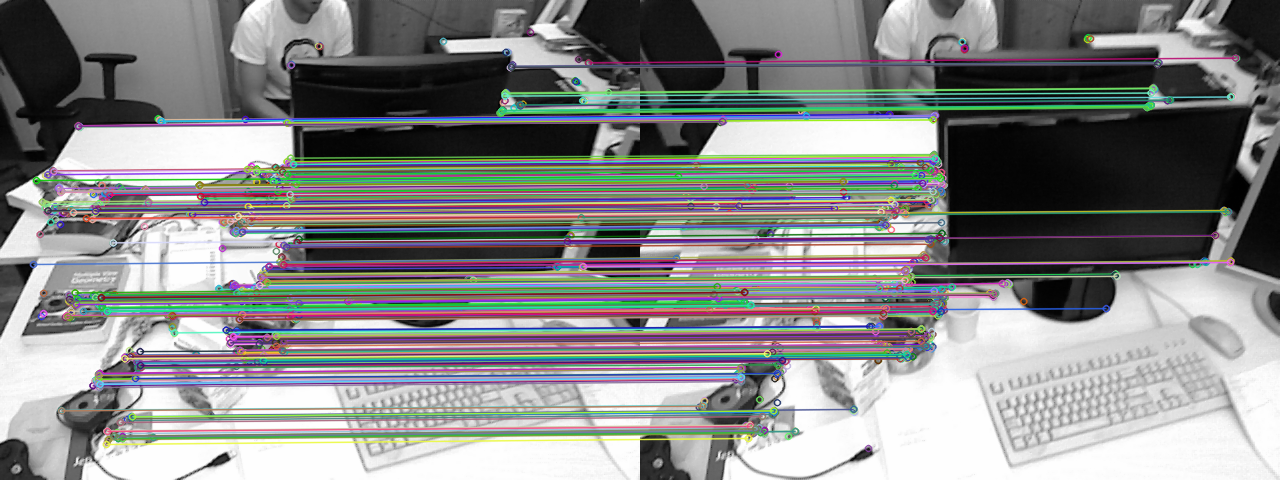
\includegraphics[width=\linewidth,natwidth=640,natheight=640]
	{fig/ref_imgs/covo_matches.png}
	\caption[ORB Feature Mathces]
	{An example feature matching scene from 
	TUM RGB-D (freiburg xyz) dataset with ORB.}
	\label{fig:feature_matchings}
\end{figure}

All being said, let's assume we pair consecutive images $(\mathbf{I}^{(k)}, 
\mathbf{I}^{(k+1)})$. In each image, we gather feature descriptors 
$(\mathbf{D}^{(1:n,k)}, \mathbf{D}^{(1:m,k+1)})$ that pass through our ORB 
filter. The goal is to find the feature correspondences based on their rotated 
BRIEF descriptor values. Again, there are many efficient ways to perform this 
matching task such as FLANN (Fast Library for Approximate Nearest Neighbors). 
Instead, in this thesis, we choose the Brute-Force matching algorithm, which 
produces fewer outliers but it is less efficient in terms of time complexity. 
The Brute-Force, as its name states, is a straightforward technique that 
compares each $\mathbf{D}^{(1:n,k)}$ descriptors in $k^{th}$ image with 
$\mathbf{D}^{(1:m,k+1)}$ descriptors in $k+1^{th}$ image by calculating 
\textit{Hamming} distance:

\begin{equation}
  d_h(\mathbf{D}^{(i,k)},\mathbf{D}^{(j,k+1)}) = \mathbf{D}^{(i,k)} \oplus \mathbf{D}^{(j,k+1)}
\end{equation}

where $\oplus$ corresponds to an 'exclusive or' logic operation. After 
calculating Hamming distances, the minimum distance are kept as best matches. 
On top of that, we perform cross-check validation by ensuring that matches 
with value $(i,j)$ such that $i^{th}$ descriptor in image $k$ has $j^{th}$ 
descriptor in image $k+1$ as the best match and vice-versa.


\section{Outlier Rejection} \label{sb_sc_ransac}

In reality, not all feature matches are correct, and it is critical that we 
detect wrong ones as the optimization algorithm that estimates the camera 
motion is sensitive to even a small number of wrong matches. In technical 
terms, we call these wrong matches \textit{outliers} (or \textit{false 
positives}). Hence, we need an algorithm to reject those outliers from 
\textit{inliers}.  The most common way is to use RANSAC \cite{Fischler1981b}, 
which is an abbreviation to Random Sample Consensus. RANSAC is an iterative 
algorithm which fits the desired model with the presence of outliers by 
selecting a subset of dataset randomly and improving parameters of model each 
iteration. Note that RANSAC works well if at least half of the dataset 
contains inliers.

\begin{figure}[H]
	\centering
	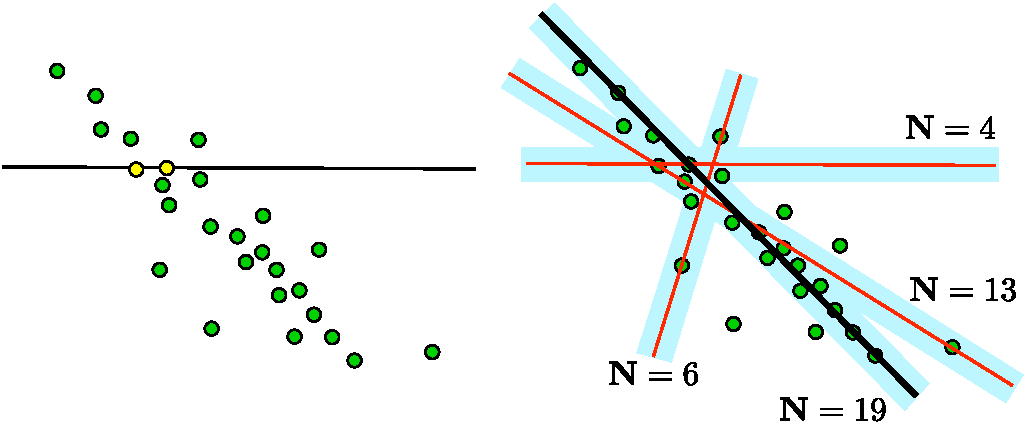
\includegraphics[width=0.8\linewidth,natwidth=640,natheight=640]
	{fig/drawings/ransac.pdf}
	\caption[Outlier Rejection with RANSAC]
	{RANSAC identifies the outliers by fitting the parameters of the 
	homography iteratively.  For simplicity, the figure depicts the outlier 
	rejection scenario with a simple line fitting example instead of 
	homography. As seen in the figure, after the number of iteration $N=14$, 
	RANSAC is able to fit line by excluding the outliers in the optimization 
	process. Note that we can still have outliers within the RANSAC inlier 
	threshold which is the area shaded with light blue color.} 
	\label{fig:outlier_matches}
\end{figure}

In section \ref{sc_pinhole}, we discussed how to model rotation and 
translation motion along with the intrinsic matrix. Parameters that we aim to 
identify are elements of projection matrix in notation 
\ref{eq:proj_func_w_square_pix_skew}.  Similarly, the model being fitted in 
RANSAC case is elements of a \textit{homography matrix}, which transforms a 2D 
image point to another 2D image point.  Remember that we have feature matches 
from image pairs. One of the pair is the transformed version of the other 
pair.  We can model this relationship in the following way:

\begin{equation}\label{eq:homography_full}
  k
  \begin{bmatrix}
    \hat{u}^{(i)} \\ \hat{v}^{(i)} \\1
  \end{bmatrix}
  =
  \mathbf{H}
  \begin{bmatrix}
    u^{(i)} \\ v^{(i)} \\1
  \end{bmatrix}
  =
  \begin{bmatrix}
    h_{00} & h_{01} & h_{02} \\
    h_{10} & h_{11} & h_{12} \\
    h_{20} & h_{21} & h_{22}
    \end{bmatrix}
  \begin{bmatrix}
    u^{(i)} \\ v^{(i)} \\1
    \end{bmatrix}
  \end{equation}

The goal is to fit parameters of $\mathbf{H}$ with the selected subset of the 
matching under the condition where majority of selected point matchings are 
inliers. In this way, we can easily detect outliers by testing whether they 
fit to model parameters or not. To make notation \ref{eq:homography_full} more 
obvious, we form linear system of equations:

\begin{equation}
\underbrace{
\begin{bmatrix}
  u^{(i)} & v^{(i)} & 1 & 0 & 0 & 0 & -\hat{u}^{(i)}u^{(i)} & -\hat{u}^{(i)}v^{(i)} -\hat{u}^{(i)}\\
  0 & 0 & 0 & u^{(i)} & v^{(i)} & 1 & -\hat{v}^{(i)}u^{(i)} & -\hat{v}^{(i)}v^{(i)} -\hat{v}^{(i)}
\end{bmatrix}}_{\mathbf{A}}
\underbrace{
\begin{bmatrix}
    h_{00} \\ h_{01} \\ h_{02} \\ h_{10} \\ h_{11} \\ h_{12} \\ h_{20} \\ h_{21} \\ h_{22}
\end{bmatrix}}_{\mathbf{h}}
= 
\begin{bmatrix}
  0\\0
\end{bmatrix}
\end{equation}

The first step of RANSAC is to select a subset that contains a minimum number 
of matching points to determine the parameters of the model. In homography 
$\mathbf{H}$ case, we need at least 4 point pairs 
$(\mathbf{u}=(u^{(i)},v^{(i)}),\mathbf{\hat{u}}=(\hat{u}^{(i)},\hat{v}^{(i)}))$
 to solve this linear system of equation. However, due to the noise, we 
require more than 4 point pairs, but this makes the problem over-determined. 
Therefore, we might find an approximated solution by solving the least squares 
problem: In doing so, we minimize so-called \textit{algebraic distance error}:

\begin{equation}
\argmin_h || \mathbf{Ah-0}||^2.
\end{equation}

In the second step, after estimating $\mathbf{h}$ parameters, we test every 
matchings that are outside the subset which randomly selected at the first 
step whether they fit to the model with the certain $\mathbf{d}$ threshold we 
define:

\begin{equation}
  ||\mathbf{\hat{u}} - \mathbf{H}\mathbf{u}||^2 > d
\end{equation}

In the third step, we include the points that passed our test procedure in the 
second step into our subset. In the fourth step, we have another test in which 
we check whether the number of matching points in our subset is large enough 
to prove that we include the majority of the inliers. If not, we go back to 
the first step and repeat the whole process until we fulfill the fourth step. 
The following listing summarizes the algorithm:

\begin{algorithm}[H] \label{algo:ransac}
  \caption{Rejecting outlier matches with RANSAC}\label{algo_ransac}

  \textbf{Input} \\
    \hspace*{\algorithmicindent}S: the smallest number of points\\
    \hspace*{\algorithmicindent}N: the number of iteration\\
    \hspace*{\algorithmicindent}d: the threshold used to identify a point which fits the model\\
    \hspace*{\algorithmicindent}T: the number of nearby points to notify that there is a good fit\\
  \textbf{Output} \\
    \hspace*{\algorithmicindent}C: the (consensus) set of inliers \\
  \begin{algorithmic}[1]

    \Procedure{RANSAC}{S,N,d,T}\\
      \While{iterations $<$ N}
      \State select random sample subset of S points
      \State estimate parameters to fit homography with S
      \ForEach {points outside S}
        \State calculate error between estimated point and measured point
        \If {error $<$ d}
          \State add point into S
        \EndIf
        \If {S $>$ T}
          \State return C $=$ S
        \EndIf
      \EndFor
      \EndWhile
    \EndProcedure
  \end{algorithmic}

\end{algorithm}

As it is seen in \ref{algo:ransac}, there are four empiric parameters that we 
need to define; S,N,d and T. In order to make the algorithm as efficient as 
possible, these parameters must be chosen carefully. As we discussed, S is the 
subset of matchings that we randomly select, and initial value should be at 
least 4 so that we can solve the least squares problem. 

For N, it is insufficient to iterate through every matching points. Thus, we 
at least select N number of matching points with respect to following 
condition:

\begin{equation}
  \text{N} = log(1-p)/log(1-(1-\epsilon)^s)
\end{equation}

where $p=0.99$ is the probability of covering all inliers, $s$ is the minimum 
number of iteration that likelihood of choosing a subset with only outliers 
and $\epsilon$ is the probability that the match is an outlier.

For d, it is chosen empirically if the distribution of outliers is unknown. If 
it is known, i.e., Gaussian with mean $\mu$ and $\sigma$, the threshold should 
be $d=5.99\sigma^2$ so that there is a 95\% probability that the point is an 
inlier.

For T, we might have a case where we reach the expected ratio of inliers; thus 
we don't have to iterate through N number of times. That means we can 
terminate it earlier if the following condition is satisfied:

\begin{equation}
  \text{T} = (1-\epsilon)n
\end{equation}

where $n$ is the total number of matching points.

It is crucial to note that we may still have outliers after RANSAC.  However, 
our motion estimation will be greatly improved since the majority of the 
outliers are removed.  Finally, we will discuss how we can utilize the 
carefully selected features and its matches to estimate the camera motion.


\section{Pose Estimation} \label{sc_pose_estimation}

Pose estimation is the core part of the VO system. After extracting and 
matching features, we finally are ready to compute \textit{transformation} 
information. The transformation corresponds to relative camera motion between 
two images that are recorded in different poses (see 
figure-\ref{fig:transformation_ij}). Let's assume; we have consecutive camera 
poses $\mathbf{x}_{k} = [\mathbf{p}_k, \mathbf{q}_k]$ and $\mathbf{x}_{k+1} = 
[\mathbf{p}_{k+1}, \mathbf{q}_{k+1}]$ where $\mathbf{p} = [p_x, p_y, p_z]^T$ 
is the position of the camera in $\R^3$ and $\mathbf{q} = [q_w, q_x, q_y, 
q_z]^T$ is the orientation of the camera in quaternion form in $SO(3)$.  
Notice that, in camera model chapter \ref{cp_cam_models}, we use rotation 
matrix to represent orientations, which made it convenient to combine 
intrinsic matrix and extrinsic matrix into a single projection matrix (see 
notation \ref{eq:simplyfied_proj_func}) so that we optimize for parameters of 
the single matrix. On the other hand, when estimating relative motion, we use 
quaternions to represent orientations, which is less intuitive way but has 
certain advantage over rotation matrix such as requiring less storage.  As a 
result, we can represent the transformation $\mathbf{T}_{k,k+1}$ $(= 
[\mathbf{t}_{k,k+1},\mathbf{q}_{k,k+1}])$ between two camera poses 
$(\mathbf{x}_k,\mathbf{x}_{k+1})$ with the rotation $\mathbf{q}_{k,k+1}$ in 
$SO(3)$  and the translation $\mathbf{t}_{k,k+1}$ in $\R^3$. That being said, 
one can formulate the transformation $\mathbf{T}_{k,k+1}$ between two camera 
pose if the initial pose $\mathbf{x}_{0}$ is known. Then, let's first find the 
camera position:

\begin{equation}
  \mathbf{p}_{k+1} = 
\mathbf{q}_{k,k+1} \otimes \mathbf{p}_k \otimes \mathbf{q}_{k,k+1}^* + 
  \mathbf{t}_{k,k+1}
\end{equation}

where $\mathbf{q}_{k,k+1} \otimes \mathbf{p}_k \otimes \mathbf{q}_{k,k+1}^*$ 
is the \textit{hamilton product} that rotates the camera position at the 
$k^{th}$ pose and $\mathbf{t}_{k,k+1}$ is the simple vector addition that 
translates the camera position. Next, the camera orientation can be found as 
follows:

\begin{equation}
  \mathbf{q}_{k+1} = 
  \mathbf{q}_{k,k+1} \otimes \mathbf{q}_{k}
\end{equation}

where $\mathbf{q}_{k,k+1} \otimes \mathbf{q}_{k}$ is the product of two 
quaternions that the former is the rotation and that the latter is the 
orientation of the camera at the $k^{th}$ pose.

\begin{figure}[H]
	\centering
  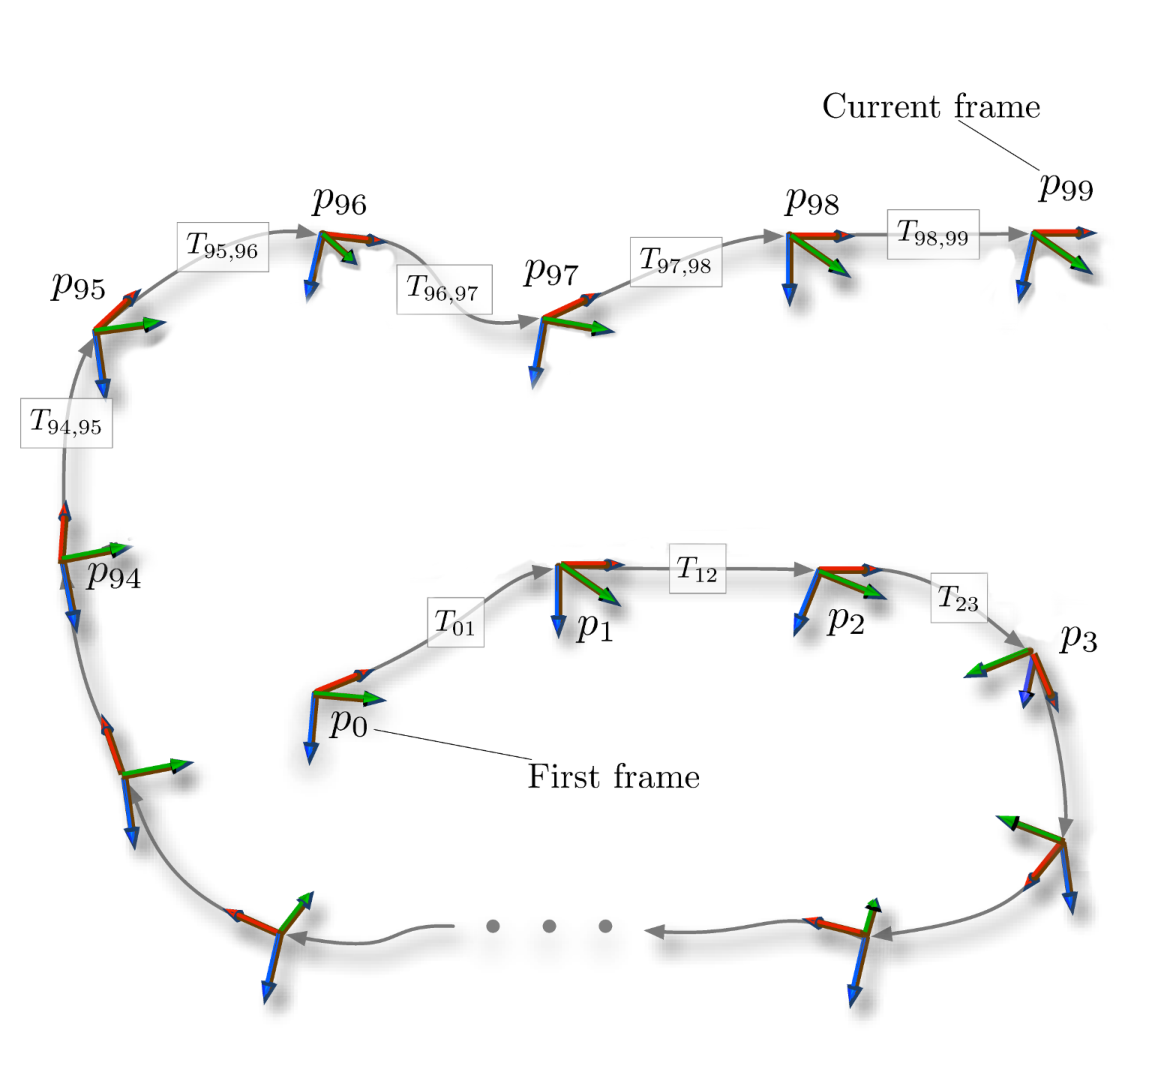
\includegraphics[width=0.7\linewidth,natwidth=640,natheight=640]
  {fig/drawings/rel_pose.pdf}
  \caption[Trajectory From Relative Pose]
  {VO estimates the ego-motion of the camera by relative poses estimated from  
  image pairs. Thus, it assumes that the initial pose $p_0$ of the camera is 
  known. Transformation $T_{0,1}$ from one image to another corresponds to the 
  camera movement from one position to another. As long as VO is able to 
  detect a sufficient number of features, it keeps estimating relative 
  transformations. With all of these transformations, one can build a 
  trajectory $(T_{0,1}, \dots, T_{98,99})$ which the camera follows.}
	\label{fig:transformation_ij}
\end{figure}

The ultimate goal in VO is to compute transformation $\mathbf{T}_{k,k+1}$ in 
multiple consecutive images and concatenate them to build a trajectory of the 
camera. As a consequence, we can track any agent on which the camera is placed 
rigidly. For example, concatenated transformation $\mathbf{T}_{0,n}$ can be 
used to calculate $n^{th}$ camera pose that is relative to the initial pose:

\begin{equation}
  \mathbf{p}_{n} = 
  \mathbf{q}_{n, n-1} \otimes (\dots
  (\mathbf{q}_{2,1} \otimes
  (\mathbf{q}_{1,0} \otimes \mathbf{p}_0 \otimes \mathbf{q_{1,0}}^* + \mathbf{t}_{1,0})
  \otimes \mathbf{q}_{2,1}^* + \mathbf{t}_{2,1})
  \dots) \otimes \mathbf{q}_{n, n-1}^* +\mathbf{t}_{n, n-1} 
\end{equation}

\begin{equation}
  \mathbf{q}_{n} = 
  \mathbf{q}_{n,n-1} \otimes \dots \otimes \mathbf{q}_{2,1} \otimes \mathbf{q}_{1,0} \otimes \mathbf{q}_{0} 
\end{equation}

To find transformation, we take advantage of image features as they can inform 
us how the camera moves if we detect them across multiple frames.  All the 
aforementioned step such as feature extraction and feature matchings are 
performed so that we can compute relative motion.  Similar to projection 
matrix \ref{eq:proj_lsq} in camera calibration, we utilize the least squares 
method for estimating an approximated transformation information due to the 
noise. 

%\subsection{Relative Pose Estimation Techniques}
%\label{sb_sc_relative_camera_pose_estimation_techniques}

So far, we discussed how we could process images so that we have adequate 
information to compute camera pose. However, we only mentioned 2D image 
features. To estimate the pose in the 3D world, we require corresponding depth 
information for features. Note that there are methods that retrieve relative 
scale information using only 2D image features and its epipolar constraints 
with monocular cameras, but we are interested in having metric depth 
information rather than relative scale in this thesis. Therefore, we have two 
common choices regarding camera types: Stereo Camera or RGB-D Camera. In our 
experiments, we experimented on RGB-D Camera to retrieve the depth information.

At this point, one generally has two ways to compute relative camera poses.  
and the reason we have different kinds of way to compute transformation arises 
from the cost function we define for the least squares problem. In the end, 
all we wish to find a good model for our optimization problem so that we 
settle on the best possible local minimum.  The design choice for cost 
function comes from the fact that we build our cost function either on $\R^2$ 
space (image plane) or $\R^3$ space (camera coordinate system).  Therefore, in 
VO literature, there are two different cost functions for modeling the least 
problem:

\begin{itemize}
  \item 3D-to-2D correspondences,
  \item 3D-to-3D correspondences.
\end{itemize}


The 2D term refers to 2D image features. Whereas, the 3D term refers to 3D 
point features that composed of back-projection of 2D features and depth 
information.  Note that this thesis does not engage with 2D-to-2D 
correspondences method since it is used in monocular camera; thus it will not 
be discussed here. On the other hand, we will discuss and compare 3D-to-2D 
correspondences and 3D-to-3D correspondences.  Although 3D-to-2D 
correspondences outperform 3D-to-3D correspondences in VO, we show the 
accuracy of 3D-to-3D correspondences can be significantly improved if the 
uncertainty of the 3D point features is modeled properly and used in the 
optimization process.  On the plus side, this technique allows us to propagate 
the uncertainty of the 3D feature points to get the uncertainty of estimated 
pose.  With being said, let's explain both methods.


\subsubsection{3D-to-2D Correspondences}\label{sb_sc_3d_to_2d}

Remember that, after feature matching step for the consecutive image frames, 
we have only2D-to-2D correspondences information and the transformation which 
we wish to compute is in $\R^3$. Therefore, we require transformation 
involving in 3D point features. That being said, we can estimate 
transformation 3D-to-2D Correspondences in four steps:

\begin{enumerate}
  \item Back-project 2D image features from $k+1^{th}$ frame to form 3D point features,
  \item Back-transform 3D point features from $k+1^{th}$ frame towards $k^{th}$ frame 
    with transformation matrix,
  \item Reproject the back-transformed 3D point features onto the $k^{th}$ image plane, 
  \item Minimize 2D Euclidean distance error between reprojected and measured 2D image features.
\end{enumerate}

\begin{figure}[H]
	\centering
  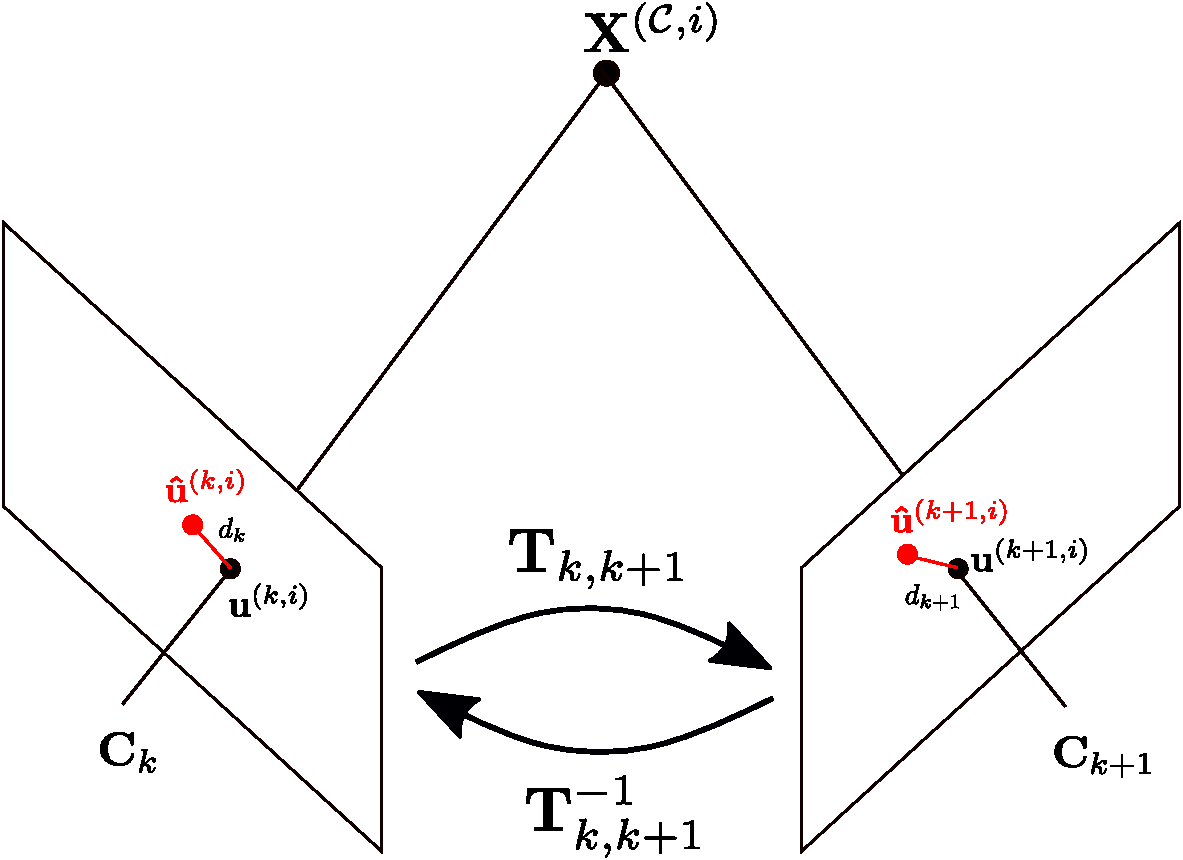
\includegraphics[width=0.9\linewidth,natwidth=640,natheight=640]
  {fig/drawings/3d_to_2d.pdf}
  \caption[3D-to-2D Correspondences]{Assuming that we have two frames taken in 
  the different poses. What 3D-to-2D correspondences method does is that it 
  takes the pixel $\mathbf{u}^{(i,k+1)}$ measurement from $k+1^{th}$ 
  back-projects to get the 3D point feature, then rotates and translates with 
  the transformation information, and projects the 3D feature to the 2D 
  feature as $\mathbf{\hat{u}}^{(i,k)}$ on image plane at $k^{th}$ frame. 
  Afterward, one will get Euclidean error distance $d_k \in \R^2$ between the 
  reprojected pixel and the measured pixel. This behavior applies for 
  reprojecting image from $k^{th}$ to $k+1^{th}$ frame to calculate $d_{k+1}$. 
  For the sake of efficiency, most VO algorithms assume that measurement 
  errors occur in only one image pair and only uses $d_k$ to minimize the 
  error, but not both $d_k+d_{k+1}$. Note that 
  this choice might decrease the accuracy of the 
  pose estimation.}
	\label{fig:min_geometric_error}
\end{figure}


To formulate the problem more clearly, let's assume we have a 3D point feature 
$\mathbf{X_c}^{(i)}=[x, y, z]^T$ in camera coordinate system and we measure 
the projections of this exact feature point as a 2D image feature, 
$\mathbf{u}^{(i,k)}=[u,v]^T$ and $\mathbf{u}^{(i,k+1)}=[u,v]^T$ on subsequent 
camera poses $k^{th}$ and $k+1^{th}$ respectively. What we also know is that 
we can back-project measured 2D image features as 3D point features using 
projection matrix (see notation \ref{eq:simplyfied_proj_func_1}) and depth 
information. Let's write again projection function that converts 3D point 
features to 2D image features: $\mathbf{u}^{(i)} = \mathbf{K}\mathbf{X}^{(i)}$.
One can also back-project 2D image features to 3D point features 
$\mathbf{K}^T\mathbf{u}^{(i)} = \mathbf{X}^{(i)} $. Now, we can formulate the 
previously discussed four steps of 3D-to-2D correspondences as follows:

\begin{enumerate}
  \item $\mathbf{X}^{(i,k+1)} = \mathbf{K}^T\mathbf{u}^{(i,k+1)}$
  \item $\mathbf{\hat{X}}^{(i,k)} = f(\mathbf{t}_{k,k+1}, \mathbf{q}_{k,k+1}, \mathbf{X}^{(i,k+1)}) = 
    \mathbf{q}_{k,k+1} \otimes \mathbf{X}^{(i,k+1)} \otimes \mathbf{q}_{k,k+1}^* + \mathbf{t}_{k,k+1} $
  \item $\mathbf{\hat{u}}^{(i,k)} = \mathbf{K}\mathbf{\hat{X}}^{(i,k)}$
  \item minimize $\sum_i||\mathbf{u}^{(i,k)} - \mathbf{\hat{u}}^{(i,k)}||^2$ where 
    $\mathbf{u}^{(i,k)}$, $\mathbf{\hat{u}}^{(i,k)} \in \R^2$
\end{enumerate}

The second and third steps can be encapsulated to a function $f$ so that 
we form the problem as an optimization problem in the following form:

\begin{equation}
  \argmin_{\mathbf{T^*}_{k,k+1} = [\mathbf{t^*}_{k,k+1}, \mathbf{q^*}_{k,k+1}]}
  \sum_i||\mathbf{x}^{(i,k)} - f(\mathbf{t}_{k,k+1}, \mathbf{q}_{k,k+1}, \mathbf{X}^{(i,k+1)})||^2
\end{equation}


\subsubsection{3D-to-3D Correspondences}\label{sb_sc_3d_to_3d}

Another way of modeling the cost function is to utilize only 3D point features 
correspondences, and one can estimate transformation with 3D-to-3D 
correspondences in three steps:

\begin{enumerate}
  \item Back-project both 2D image features from $k^{th}$ and $k+1^{th}$ 
  frames as 3D point features, 
  \item Back-transform the back-projected 3D point features from $k+1^{th}$ 
  frame,
  \item Minimize 3D Euclidean error distance between back-transformed and 
  measured 3D point features.
\end{enumerate}

\begin{figure}[H]
	\centering
	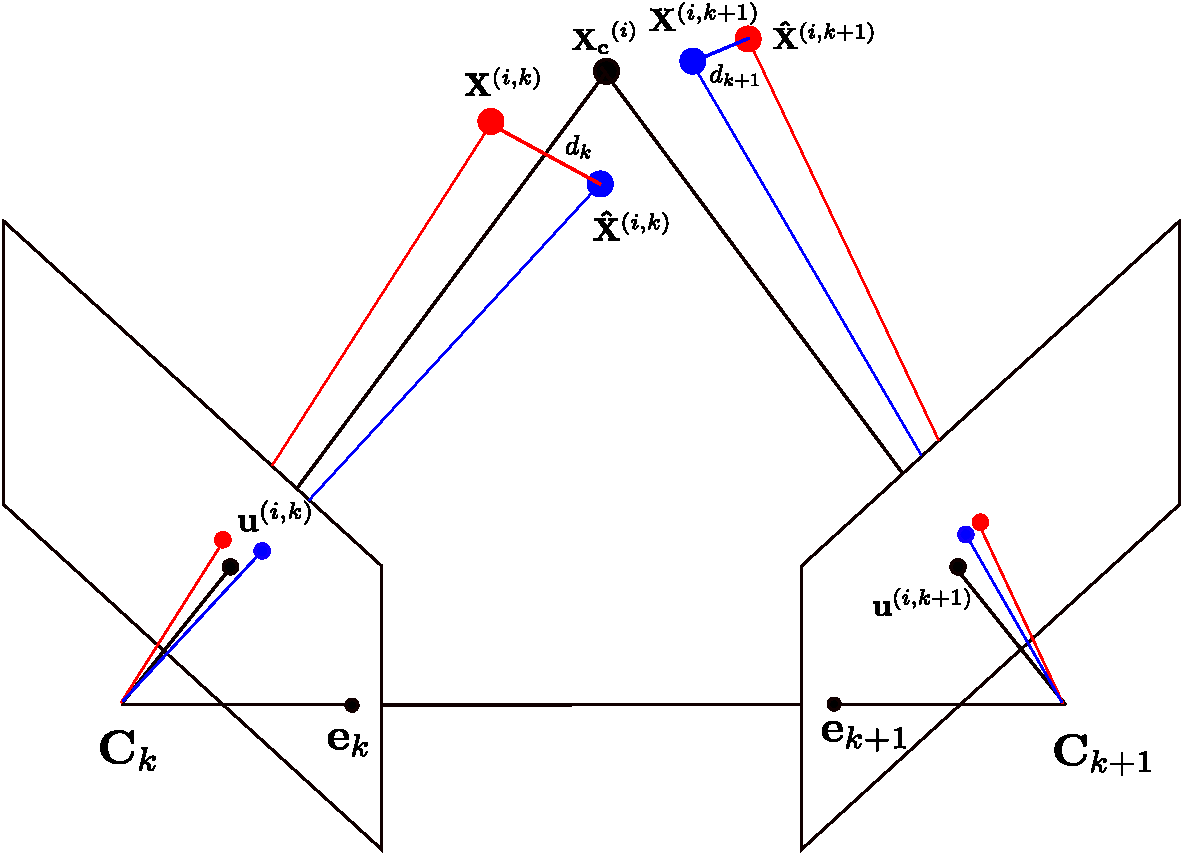
\includegraphics[width=0.9\linewidth,natwidth=640,natheight=640]
	{fig/drawings/3d_to_3d.pdf}
	\caption[3D-to-3D Correspondences]
	{3D-to-3D correspondences method calculates the Euclidean error distance 
	in 
	3D space. For example, all image features 
	$\mathbf{u}^{(i,k)},\mathbf{u}^{(i,k+1)}$ from both frames are 
	back-projected to get 3D point features 
	$\mathbf{X}^{(i,k)},\mathbf{X}^{(i,k+1)}$. Then, $\mathbf{X}^{(i,k+1)}$ is 
	rotated and translated with the transformation information 
	$\mathbf{T}_{k,k+1}$ to align the same 3D point feature 
	$\mathbf{\hat{X}}^{(i,k)}$ with respect to $k^{th}$ camera's centre.In 
	this 
	way, one can calculate the Euclidean distance error $d_k \in \R^3$.Reverse 
	behavior applies on moving features from $k^{th}$ to $k+1^{th}$ frame to 
	calculate $d_{k+1}$ as well.}
	\label{fig:min_euclidean_error}
\end{figure}


The similar formulation that we previously did for 3D-to-2D correspondences 
applies for the 3D-to-3D correspondences as well but only with few changes. 
Let's again assume that we have two corresponding 2D image features, 
$\mathbf{u}^{(i,k)}$ and $\mathbf{u}^{(i,k+1)}$. However, rather than 
minimizing error on the 2D image plane, we want to minimize them on 3D space. 
Therefore, we need to back-project both image features. With that in mind, we 
can formulate the three steps of 3D-to-3D correspondences as follows:

\begin{enumerate}
  \item $\mathbf{X}^{(i,k+1)} = \mathbf{K}^T\mathbf{u}^{(i,k+1)}$ and 
    $\mathbf{X}^{(i,k)} = \mathbf{K}^T\mathbf{u}^{(i,k)}$ 
  \item $\mathbf{\hat{X}}^{(i,k)} = f(\mathbf{t}_{k,k+1}, \mathbf{q}_{k,k+1}, \mathbf{X}^{(i,k+1)}) = 
    \mathbf{q}_{k,k+1} \otimes \mathbf{X}^{(i,k+1)} \otimes \mathbf{q}_{k,k+1}^* + \mathbf{t}_{k,k+1}$
  \item minimize $\sum_i||\mathbf{X}^{(i,k)} - \mathbf{\hat{X}}^{(i,k)}||^2$ where $\mathbf{X}^{(i,k)}$, $\mathbf{\hat{X}}^{(i,k+1)} \in \R^3$

\end{enumerate}

The second step can be encapsulated to a function $f$ to form the optimization 
problem:

\begin{equation}
  \argmin_{\mathbf{T^*}_{k,k+1} = [\mathbf{t}_{k,k+1}, \mathbf{q}_{k,k+1}]}
  \sum_i||\mathbf{X}^{(i,k)} - f(\mathbf{t}_{k,k+1}, \mathbf{q}_{k,k+1}, \mathbf{X}^{(i,k+1)})||^2
\end{equation}\label{eq:3d_to_3d_rel_pose_est}

In VO literature, this method is usually discarded since it performs poorly 
comparing to 3D-to-2D correspondences. However, we prove that it can be 
improved if feature covariances are properly estimated and included in the 
optimization problem.


% ***************************CP3-MOTIVATION***************************
\chapter{Motivation} \label{cp_motivation}

The essence of a mobile robot is autonomy. 
A fully autonomous robot first \textit{senses} its environment, then 
\textit{interprets} the collected data and finally \textit{acts} based on the insights 
that it gathered over time.
If we look at nature, throughout the evolution, 
certain animals gained certain abilities regarding 
spatial awareness in all sorts of ways. For instance, 
homing pigeons navigate by magnetic field, bats use sound to map their 
surroundings or bees smell with their special chemoreception to find their way 
back home. 
Even though each sense helps us with particular importance,
we humans are good at navigating ourselves by relying on our vision. 
As the incredible capability of a human eye (locating and recognizing 
objects within milliseconds even in ambiguous situations) stays a mystery, 
robotics researchers has always been keen on exploiting the computer vision field, 
especially Visual Odometry and Visual SLAM.

Visual Odometry outputs relative ego-motion information similar to IMU and 
wheel odometry. Apart from absolute sensor measurments like known a priori set of landmarks
or GPS, all of three low-level sensors are heavily used in 
localization applications as relative sensors. 
Nowadays, sensor fusion applications like SLAM and 3D reconstruction are designed 
accordingly to compensate each other's biases in order to obtain the best 
possible result. In the case of an accurate and robust sensor fusion framework, 
one selects sufficient amount absolute and relative positioning sensors. 
The ultimate goal is to fuse both relative and absolute sensor types 
along with their noise characteristics in a way that the error is minimized. 
Hence, it is critical to model each sensor's uncertainties. 
IMU and wheel odometry sensors' uncertainty are modeled by their vendors 
based on the working principles and worst-case scenario tests beforehand.
Whereas, widely used open source VO tools do not provide any uncertainty information 
about their pose estimations. Even though there are several VO papers 
\cite{Endres2014}, \cite{Konolige08}, \cite{Di2016a}, \cite{Belter2018a}
that deals with uncertainty of RGB-D sensors, they only intend to 
improve accuracy of the pose estimation, but not to provide any uncertainty 
information about their estimation. Therefore, my aim, in this thesis, is to build 
a feature-based RGB-D Visual Odometry system that outputs pose estimations 
along with their metric uncertainties.
As a result, VO system can be treated as a low-level 
relative motion sensor in a sensor fusion application.

% ***************************CP4-CoVO***************************
\chapter{An Error-Aware RGB-D Visual Odometry} \label{cp_covo}

\section{Related Work} \label{sc_error_aware_visual_odometry_related_works}

An \textit{error-aware} Visual Odometry estimates an ego-motion of a camera
along with the uncertainty of its estimations.  Remember that the primary goal
of a sensor fusion application is to combine multiple sensors to get a better
estimation of its pose.  In this case, we need metric uncertainty
representation for each sensor.  That is why we require a covariance matrix for
every pose estimation from all sensors so that we can compensate sensors'
biases dynamically throughout the trajectory.  Ideally, a good error-aware VO
system should tell us how confident its pose estimation at a specific time
instance by taking factors, such as a number of detected features and their
noises, into account.

To build such an error-aware VO with an RGB-D camera, one needs to be able to
model the noise characteristics of the sensor used in the camera. The passive
stereo camera and its error propagation application for the uncertainty
estimation are already well-studied problems in \cite{Leo2011} and
\cite{Miura1993AnUM}.
% Uncertainty Model for Stereo Cam
% - Leo2011 - Covariance Propagation for the Uncertainty Estimation in Stereo
%   Vision
% - Miura1993AnUM - An Uncertainty Model of Stereo Vision and its Application
%   to Vision-Motion Planning of Robot
However, in this thesis, I am interested in implementing the spatial error
propagation of the active stereo for the VO application since there is, to my
knowledge, little work being done.

Because our VO algorithm is a feature-based technique, the uncertainty of image
features must be modeled.  Generally, this is known as a quantization error
referring to a pixel noise \cite{RichardHartley2003} which is assumed to be
maximum half pixel and normally distributed in literature.  To represent the
pixel uncertainty of features in the 3D world, the conic ray model
\cite{Sola2007a} is used by build on the pinhole model of a camera.
%However, this model can only cover uncertainties on image plane axes that are
%perpendicular to the camera coordinate system.  Conic Ray Model For Feature
%Pixel Uncertainty
% - RichardHartley2003 - Multiple View Geometry
% - Sola2007a - Towards Visual Localization, Mapping and Moving Objects
%   Tracking by a Mobile Robot: A Geometric and Probabilistic Approach

Moreover, one should consider depth uncertainty as well. In this perspective,
In \cite{Mallick2014b}, authors gathered existing studies about the depth
camera's noise of Kinect. Since Kinect has two version that uses different
technologies for measuring depth information, researchers compared the
performance of both versions in \cite{Wasenmuller2017b} and \cite{Kinect2015}.
%Note that we use Kinect V1 which uses the structured light in our experiments.
Another extensive study is \cite{Khoshelham2012a}, outlining both a theoretical
and experimental background for accuracy and resolution of the Kinect's depth
camera based on the geometrical model.  Conversely, \cite{Choo2014} conducts a
comprehensive statistical analysis to build a high-order polynomial
mathematical model for the standard deviation of depth error.
% Kinect Depth Noise Model
% - Mallick2014b - Characterizations of noise in Kinect depth images: A review
% - Wasenmuller2017b - Comparison of Kinect v1 and v2 depth images concerning
%   accuracy and precision
% - Kinect2015 - Kinect Range Sensing: Structured-Light versus Time-of-Flight
%   Kinect
% - Khoshelham2012a - Accuracy and resolution of Kinect depth data for indoor
%   mapping applications
% - Choo2014 - Statistical Analysis-Based Error Models for the Microsoft

Even though the studies \cite{Park2012a} and \cite{Nguyen2012a} that deals with
Kinect model the uncertainty, they don't utilize them on a VO system. In
\cite{Park2012a}, the author contributed an important methodology on how to
model confidence ellipsoids of 3D point features measured by Kinect. In this
paper, the standard deviation of the depth noise is assumed to be constant.  In
fact, it increases with distance from camera quadratically. \cite{Nguyen2012a},
however, addresses this issue by defining a quadratic function whose parameters
are identified with the optimization process.  They even evaluate the
performance of their proposed model for pose estimation, which is quite
relevant to our task, but settings of their experimentation are unclear since
they focus mostly on 3D reconstruction.

For applications such as SLAM and 3D Reconstruction, there are other papers
\cite{Endres2014}, \cite{Konolige08}, \cite{Di2016a} that incorporate
uncertainty models, but they assume half pixel Gaussian noise for all features.
Naturally, this increases their localization accuracy. However, it still
unclear how one can propagate covariance of the detected features to the
covariance of the estimated pose in the presence of outliers of matched
features.  The only exception that attempts to model the pixel uncertainty of
features is \cite{Belter2018a}.  They implemented a so-called reserve-SLAM
simulation tool to identify the pixel noise caused by feature descriptor.  They
too did not propagate feature covariance to get pose covariance.  They only
used features covariance to improve pose estimation accuracy.  In this thesis,
I am interested in propagating the covariance of the matched features to the
covariance of the estimated camera pose in the presence of outliers.
% Similar Implementations
% - Park2012a - Spatial Uncertainty Model for Visual Features Using a Kinect™
%   Sensor
% - Nguyen2012a - Modeling kinect sensor noise for improved 3D reconstruction
%   and tracking
% - Endres2014 - 3D Mapping with an RGB-D Camera
% - Konolige08 - FrameSLAM : From Bundle Adjustment to Real-Time Visual Mapping
% - Di2016a - RGB-D SLAM based on extended bundle adjustment with 2D and 3D
%   information
% - Belter2018a - Modeling spatial uncertainty of point features in
%   feature-based RGB-D SLAM

\section{Implementation Details of CoVO}

CoVO (Covariance-enabled Visual Odometry) is the proposed error-aware VO
algorithm based on an RGB-D camera.  It utilizes 3D-to-3D correspondences
method along with the uncertainty of 3D point features to estimate relative
camera poses. Most importantly, it exploits the metric covariance of 3D point
features to propagate the pose covariance.  An overview of the CoVO pipeline is
illustrated in figure \ref{fig:covo_pipeline}.

\begin{figure}[H] \centering
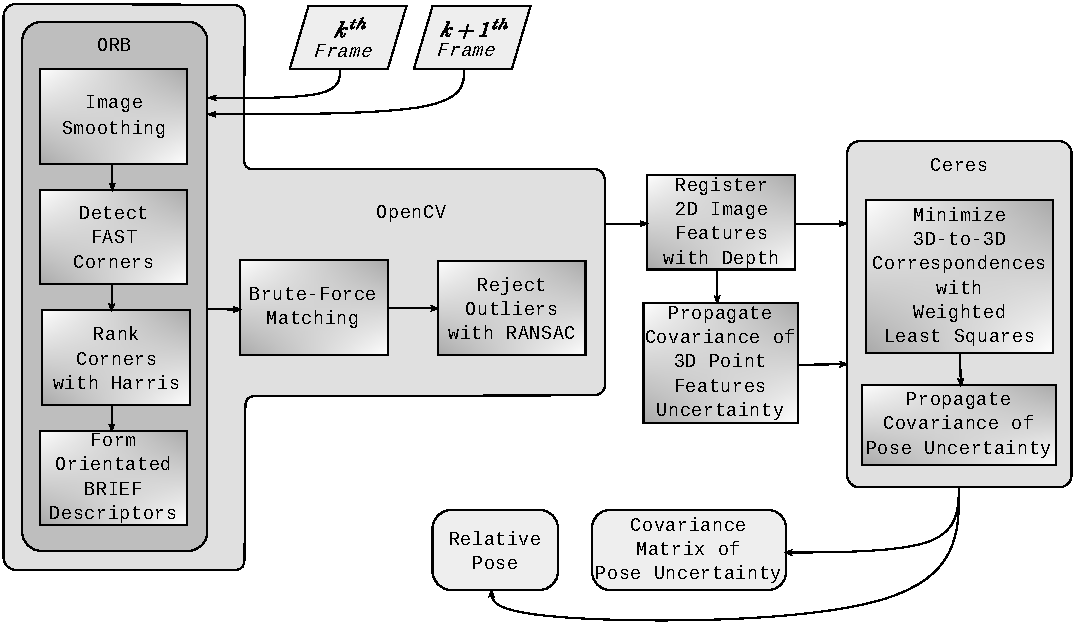
\includegraphics[width=0.9\linewidth,natwidth=640,natheight=640]
{fig/drawings/covo.pdf} \caption[CoVO Pipeline]{CoVO: The source code of the
implementation can be found in:
\href{https://github.com/ugurbolat/CoVO}{https://github.com/ugurbolat/CoVO}}
\label{fig:covo_pipeline} \end{figure}

Many VO systems require parameter tuning process and have algorithmic
variations.  Thus, building a reliable VO can be a daunting task.  To minimize
implementation errors and development time, we take advantage of two commonly
used open source libraries; i.e., OpenCV (\cite{opencv}) for handling image
feature manipulations and Ceres (\cite{ceres-solver}) for optimization. We
chose these two libraries because they are mature open source projects that
ensure efficiency and allow required customization.  In the following part of
this section, we will explain the essential steps that we take to build CoVO:


\begin{enumerate} 
  \item \textbf{Extracting Feature:} We choose ORB due its efficiency and
    repeatability. Before extracting ORB features, we convert RGB images to
    grayscale. Then, we detect corners with FAST-9 that takes a patch of
    circular radius as 9 pixels around the corner. Next, the detected corners
    are ranked with Harris filter according to their image derivatives. In this
    way, we can query top N corners.  Finally, orientated BRIEF descriptors are
    formed by randomly selected pairs.  Note that these functionalities are
    already available in OpenCV and they are built based on \cite{Rublee2011a}.  
  \item \textbf{Matching Features:} After extracting ORB features from
    consecutive images, we matched them with Brute-Force algorithm that uses
    Hamming window for the comparison. Before calling two features as a match,
    the cross-check is performed to make sure both features are identified as a
    match in their own comparison set.  In the end, a filtering operation is
    applied on the matches by removing worst 10\% matches based on the distance
    calculated by Hamming window.
  \item \textbf{Rejecting Outliers:} With the remaining matches, we apply
    RANSAC to reject outliers. Note that we choose RANSAC threshold to be 10
    pixels. Also, remember that we will have pseudo inliers even after applying
    RANSAC and the pixel errors are not particularly bounded with 10 pixels.
    The effect of pseudo inliers in pixel uncertainty is discussed in section
    \ref{sc_pseudo_inliers}.
  \item \textbf{Register 2D Features With Depth:} At this step, we simply
    combine inlier 2D features with their corresponding depth information. It
    is critical to note that Kinect has invalid depth measurement which is
    measured as 0 disparity level for certain regions of the object surface.
    Thus, we remove 2D features having invalid depth value from match set.
    Plus, we remove 2D features that have a depth value greater than $5m$ since
    it is Kinect's accurate depth distance range. 
  \item \textbf{Preparing Covariance Matrix of 3D Feature Points:} For every
    inlier matched features, we propagate pixel uncertainties
    $\mathbf{Q_{uvz}}$ from image plane to camera coordinate system
    $\mathbf{Q_{xyz}}$ with the Jacobian of back-projection function
    $\mathbf{J_{bp}}(\mathbf{u})$ (see notation \ref{eq:cov_xyz_prop}). This
    step is crucial for both improving for pose estimation results and
    estimating pose covariance.  
  \item \textbf{Minimizing 3D-to-3D Correspondences With Weights:} To able to
    take advantages of feature covariances of both consecutive images, we
    expand the residuals by defining both back- and forward transformation
    function (see notation \ref{eq:residuals_w_back_and_forward}).  It improves
    the optimization process because we take measurement error in both images.
    The technique is taken from [\cite{RichardHartley2003}, p.101].  Then, the
    weighted least squares problem is solved by Levenberg-Marquardt by
    minimizing the error between 3D-to-3D correspondences to calculate relative
    camera pose.  
  \item \textbf{Calculating Covariance Matrix of the Estimated Pose:} After
    completing least squares optimization process, we calculate the covariance
    $\mathbf{Q_{tq}}$ of the estimated relative camera pose by propagating it
    from the feature covariances $\mathbf{Q_{xyz}}$ with the Jacobian of
    residuals function $\mathbf{J'}(\mathbf{x^*})$ at the optimal solution (see
    notation \ref{eq:cov_tq_prop}).  Due to the non-linearity of the projection
    function, an approximated version of the error propagation law produces
    overconfident covariance estimations. Thus, we scale the resulting
    $\mathbf{Q_{tq}}$ with $\phi$ to keep the estimator conservative.  The
    reason why we have this heuristic parameter is discussed in section
    \ref{sc_cov_eval}.  
\end{enumerate}

Note that all of the parameters mentioned above of CoVO are given as a list in
appendices \ref{sc_covo_tuning_param}.  In the end, building such a VO system
require many tuning parameters and many VO algorithms do not emphasize the
effect of this phenomena.  The fact that we aim to develop an error-aware VO
that produces metric pose covariances means that each parameter must be
examined.  In the following sections of this chapter, we will discuss the
necessary components and parameters of the CoVO pipeline to highlight what is
required for an error-aware system.

\section{Modeling Uncertainty of RGB-D Camera} \label{sc_modeling_uncertainty_of_rgbd}

The main reason why conventional VO applications do not provide any uncertainty
information (namely covariance matrix) for its pose estimation is that it is
hard to model error characteristics of the whole VO pipeline.  This is because
we perform many preprocessing, each of which eventually introduces different
types of error. What we aim is to define potential error source of the VO and
to model them. Thus, we will investigate the noise characteristic of sensors in
RGB-D camera in this section. In particular, we examine Kinect, having three
sensors: RGB camera, IR camera, and IR laser projector.  In our experiments and
evaluations, we assume that these sensors are calibrated such that there is no
registrations error when mapping RGB pixels to disparity pixels.

Furthermore, we assume that measurements with these sensors are independent of
each other.  Under this assumption, we split the source of errors into two
categories: feature related and depth-related uncertainties. The former is
caused by point feature location and matching algorithms. The latter is caused
by the depth camera sensor.  Let's see how we can model these two error sources
and how to form an uncertainty model for Kinect so that we estimate
metric covariance matrices for each relative camera pose.

\subsection{Feature Related Uncertainty} \label{sb_sc_pixel_uncertainty}

Our VO pipeline heavily relies on the detected features. For a VO algorithm to
operate reliably, it is expected that you will have a video stream that has
small translation and rotation differences at the consecutive images. Thus,
when pairing images to find common features, we expect not to have high-degree
rotation or a large amount of scaling on image features so that matching
algorithm would not suffer from a high number of outliers. Under these
circumstances, we identify two main error sources related to features; i.e.,
interest point location uncertainty and outliers in feature matching.


To understand these two types of errors, we need to remind ourselves how we
detect and describe features section \ref{sc_feature_extraction} in the first
place.  In ORB, FAST corner filter is performed by selecting pixel coordinates
of an interest point and comparing it with its surrounding pixels. In an ideal
scenario where we match features in consecutive image perfectly, we would
assume that the error will be a half pixel due to the quantization process of
the RGB camera.  The ideal scenario breaks once we have outliers. 
In other words, if we had perfect matches, all the reprojected features would
be situated closely to their matches and the error distance between matches
would be a half pixel. However, we still have outliers even after applying
RANSAC. Thus, the error distance for those outliers would be greater that one
pixel.  In this thesis, we call those outliers that appear after RANSAC
\textit{pseudo inliers}. Moreover, instead of taking pixel errors a half pixel,
we investigate the pixel error caused by pseudo inliers in section
\ref{sc_pseudo_inliers} and treat them as pixel uncertainty.

\begin{figure}[H] \centering
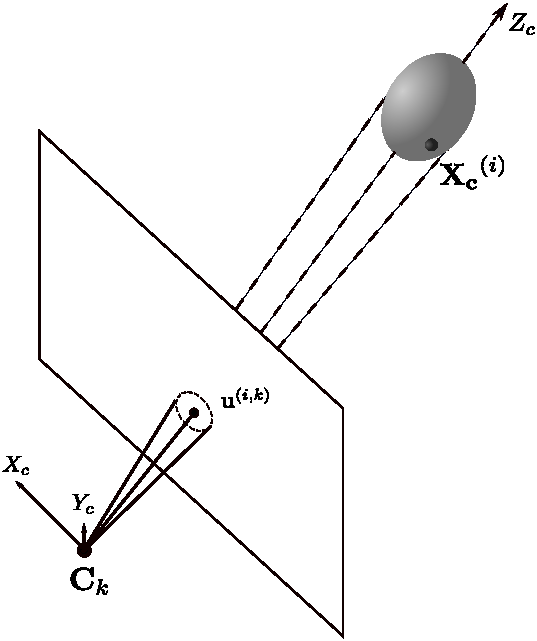
\includegraphics[width=0.6\linewidth,natwidth=640,natheight=640]
{fig/drawings/conic_ray.pdf} \caption[The Conic Ray Error Model]{ The conic ray
model is inspired from \cite{Sola2007a} and we expand a confidence ellipse to a
confidence ellipsoid by adding depth uncertainty since we use a RGB-D camera.}
\label{fig:conic_ray_3d_error_model} \end{figure}

Having all these in mind, let's model uncertainty related to features.  First
of all, remember that 3D point features in the camera coordinate system are
projected to 2D points on an image plane with the pinhole model from section
\ref{sc_pinhole}.  When the aperture of a digital camera opens, it captures
incoming light rays using its light detector sensor (typically CMOS image
sensors) and turns them into electrical signals, which is an over-simplified
definition of a camera. With the help of the pinhole model, one can build a
model for light ray coming from a 3D point.  Because we have the errors as
mentioned above, we can't measure the exact location of the 3D point feature.
However, it is likely that the point is within the dash line region (see figure
\ref{fig:conic_ray_3d_error_model}) As a consequence, we form an uncertainty
region which we call \textit{conic ray}.  Within this conic ray, we can
represent the uncertainty of a point with a \textit{confidence} ellipsoid if
the depth uncertainty is included.  To formulate this uncertainty, we need to
find parameters of the confidence ellipsoid which can be represented with
multi-dimensional Gaussian distributions in 3D space:

\begin{equation} \mathbf{g}_{xyz}(\mathbf{X}^{\mathcal{C}}) =
\frac{1}{\sqrt{(2\pi)^3|\mathbf{Q_{xyz}}|}} \exp(-\frac{1}{2}
(\mathbf{X}^{\mathcal{C}}-\mathbf{m_x}^{\mathcal{C}})^\intercal
\mathbf{Q_{xyz}}^{-1} (\mathbf{X}^{\mathcal{C}}-\mathbf{m_x}^{\mathcal{C}}))
\end{equation} \label{eq:cov_ellipse}

where $\mathbf{X}^{\mathcal{C}} = \begin{bmatrix} x \\ y \\ z\end{bmatrix}$ is
the real position of the point in the camera coordinate system,
$\mathbf{m_x}^{\mathcal{C}} = \begin{bmatrix} m_x \\ m_y \\ m_z \end{bmatrix}$
is the measured position, and $\mathbf{Q_{xyz}} = \begin{bmatrix} \sigma_x^2 &
\sigma_x\sigma_y & \sigma_x\sigma_z \\ \sigma_y\sigma_x & \sigma_y^2 &
\sigma_y\sigma_z\\ \sigma_z\sigma_x & \sigma_z\sigma_y &
\sigma_z^2\end{bmatrix}$ is the covariance of measurement error.  Notice that
errors in $x,y$ and $z$ direction are correlated to each other as the ellipsoid
can be tilted with respect to the focal point of the camera.  With regards to
measurement error in $x$ and $y$ direction, we only have indirect knowledge
since we measure features on image plane in $u$ and $v$ direction.  As to
measurment error in $z$ direction, we have direct knowledge (we assume that
disparity data is already converted to depth information).  As a matter of
fact, $(u,v,z)$ form a special space $\R^3$ called \textit{disparity image
space}.  To get errors in $x$ and $y$ directions, we need to propagate pixel
uncertainties from image plane to camera coordinate system. Thus, we remind
ourselves with the back-projection function:

\begin{equation} \mathbf{X}^{\mathcal{C}} = \mathbf{F_{bp}}(\mathbf{u})
\end{equation}

\begin{equation} \begin{bmatrix} x \\ y \\ z \end{bmatrix} = \begin{bmatrix}
\frac{z}{f_x} & 0 & -\frac{z c_x}{f_x} \\ 0 & \frac{z}{f_y} & -\frac{z
c_y}{f_y} \\ 0 & 0 & z \end{bmatrix} \begin{bmatrix} u \\ v \\ 1 \end{bmatrix}
\end{equation}

One can represent the probability distribution of the pixel and depth error
with another multivariate Gaussian distribution formed by pixel uncertainties. 

\begin{equation} \mathbf{g}_{uvz}(\mathbf{X}^{\mathcal{D}}) =
\frac{1}{\sqrt{(2\pi)^3|\mathbf{Q_{uvz}}|}} \exp(-\frac{1}{2}
(\mathbf{X}^{\mathcal{D}}-\mathbf{m_u}^{\mathcal{D}})^\intercal
\mathbf{Q_{uvz}}^{-1} (\mathbf{X}^{\mathcal{D}}-\mathbf{m_u}^{\mathcal{D}}))
\end{equation} \label{eq:cov_ellipse}

where $\mathbf{X}^{\mathcal{D}} = \begin{bmatrix} u \\ v \\ z\end{bmatrix}$ is
the real pixel coordinates and the corresponding depth value in disparity image
space, $\mathbf{m_u}^{\mathcal{D}} = \begin{bmatrix} m_u \\ m_v \\ m_z
\end{bmatrix}$ is the noisy pixel measurements along with the noisy depth
measurement, and $\mathbf{Q_{uvz}} = \begin{bmatrix} \sigma_u^2 & 0 & 0\\ 0 &
\sigma_v^2 & 0 \\ 0 & 0 & \sigma_z^2\end{bmatrix}$ is the covariance of these
measument errors as pixel and depth measurements are considered independent.

To convert disparity image space to camera coordinate system, we utilize the
error propagation low. In this respect, we need the partial derivative of the
back-projection function:

\begin{equation} \mathbf{J_{bp}}(\mathbf{u}) = \frac{\partial
\mathbf{F_{bp}}(\mathbf{u})}{\partial \mathbf{u}}  = \begin{bmatrix}
\frac{z}{f_x} & 0 & (\frac{u}{f_x} - \frac{c_x}{f_x}) \\ 0 & \frac{z}{f_y} &
(\frac{v}{f_y} - \frac{c_y}{f_y}) \\ 0 & 0 & 1 \end{bmatrix} \end{equation}

Then, we propogate the pixel covariances as follows:

\begin{equation} \mathbf{Q_{xyz}} = \mathbf{J_{bp}}(\mathbf{u})^T
\mathbf{Q_{uvz}} \mathbf{J_{bp}}(\mathbf{u}) \end{equation}


Apart from pixel uncertainties, what we haven't discussed is how we get the
$\sigma_z$ depth uncertainty.  It deserves own explanation so we will cover in
the next section.

\subsection{Depth Related Uncertainty} \label{sb_sc_depth_uncertainty}

Modeling noise in depth measurements is more complicated than an RGB camera.
In section \ref{sc_depth_model}, remember that we explained how structured IR
light speckles are projected onto an object so that IR camera can capture its
deformed patterns.  During this process, many things can go wrong. For example,
(1) specific ambient background would make Kinect suffer from over-saturated
disparity image, (2) having multiple Kinect in the same environment can lead to
interference issue, (3) multi-path propagation of the light might change the
expected illumination, or (4) measuring in dynamic scene might result in
improper IR light patterns. All of these non-deterministic events makes it
harder to model the uncertainty. However, we assume that operating conditions
and environment are chosen carefully to avoid these events as much as possible.
What we aim to model in this section is mostly systematic errors in Kinect. In
this regard, we rely on the experiments conducted by \cite{Nguyen2012a}. 

\subsubsection{Kinect's Systematic Depth Noise}

The experimental analysis contributed to model Kinect's depth noise.
\cite{Nguyen2012a} calculated the difference between ground truth and Kinect
measurements and,  found out that there are two types of systematic noise
occurring in Kinect's depth measurements: \textit{axial} noise and
\textit{lateral} noise.  Note that our depth noise model is based on their
work.


\begin{figure}[H] \centering
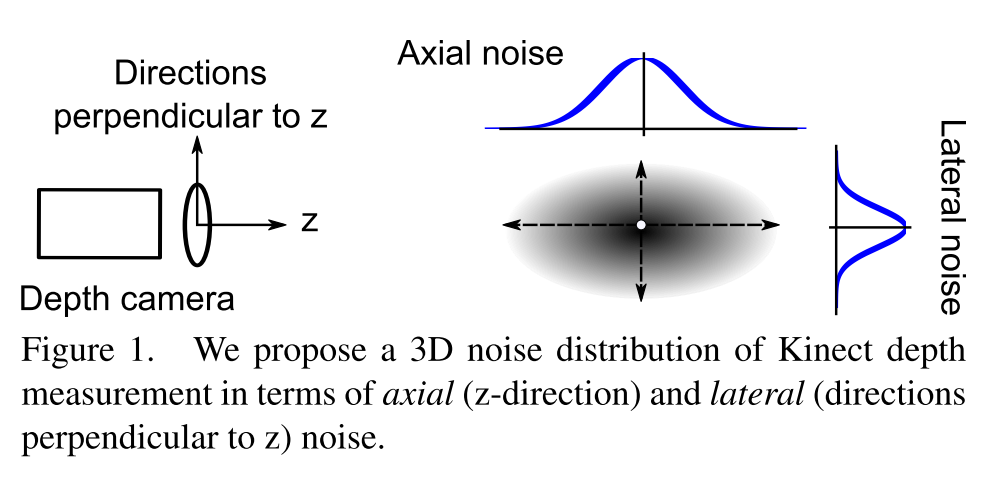
\includegraphics[width=0.7\linewidth,natwidth=640,natheight=640]
{fig/ref_imgs/kinect_noise_model.png} \caption[Kinect's Depth Noise
Model]{According to \cite{Nguyen2012a}, axial noise corresponds to noise along
the $z$ axis in the camera coordinate system. In other words, it is the depth
uncertainty model we search for our conic ray model.  On the other hand,
lateral noise corresponds to directions perpendicular to the $z$ axis. This
noise creates an uncertainty in the pixel coordinates of the disparity image.
The figure is taken from \cite{Nguyen2012a}.} \label{fig:kinect_noise_model}
\end{figure}

To detect the lateral and axial noise, they built an experimental setup with a
Kinect that projects its IR speckle patterns onto a planar surface.  Then, they
collected depth measurements at a different distance to the planar surface
positioning at different angles.  For calculating the axial noise, they first
removed the lateral noise cropping edges. Then, remaining depth region was
fitted to a plane that has the minimum error to the ground truth. Finally, they
calculated distance difference between measured depth and ground truth.
Whereas, the lateral noise was simply calculated by taking pixel difference
between fitted straight edge passing through the center of distribution and
measured (zigzag-like shape) pixels. The illustration of this experiment is
given in figure \ref{fig:kinect_noise_experiment}.

\begin{figure}[H] \centering
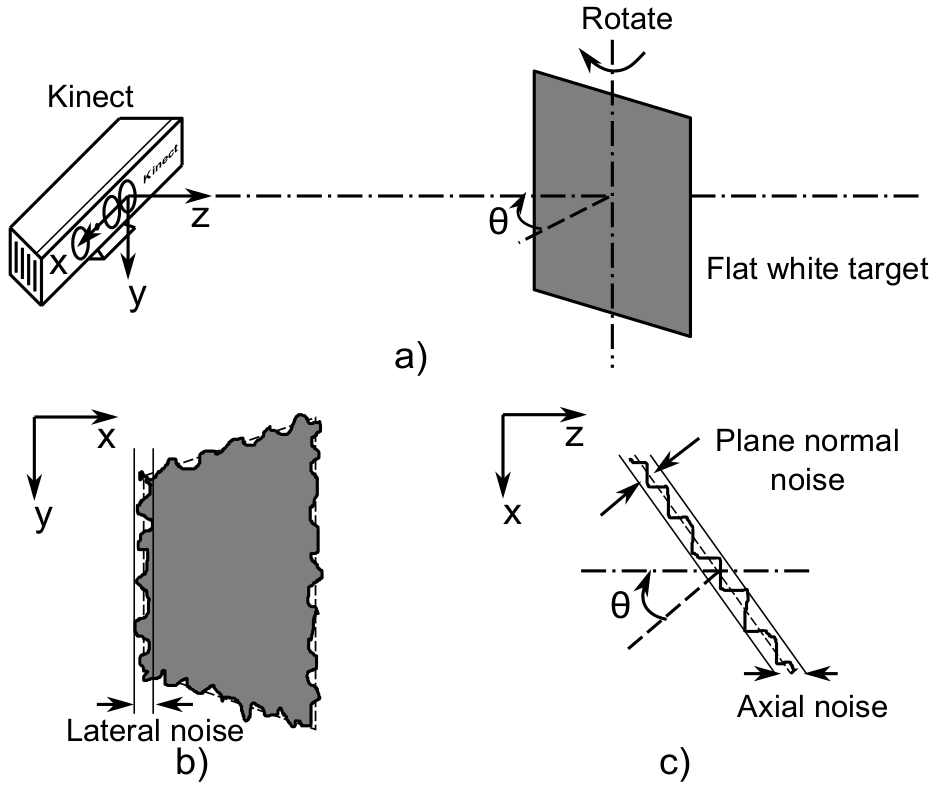
\includegraphics[width=0.7\linewidth,natwidth=640,natheight=640]
{fig/ref_imgs/kinect_noise_experiment.png} \caption[Kinect's Depth Noise
Experiment]{In order to measure the depth noise, an object that has flat white
surface was placed at different known distances to Kinect. During the
experiments, they also discovered that depth noise changes when the angle of
the object changes with respect to Kinect's focus point. Thus, they included
different poses with different angles by rotating the object (a).  The effect
of lateral and axial noise is depicted in (b) and (c).  The figure is taken
from \cite{Nguyen2012a}.} \label{fig:kinect_noise_experiment} \end{figure}

After calculating errors between measurements and ground truth, they realized
that the axial and lateral noise have different noise characteristics. The
lateral noise error distribution stays constant with the distance, while the
axial noise distribution gets wider with the increased range.

Besides, the axial noise has another property, which is the response to the
different angles. It was observed that the standard deviation of the axial
noise increases drastically after 60 degrees.  In the light of these
experiments, they proposed two empirical models that fit corresponding
measurements for the axial and lateral noise.  For axial noise, they define a
quadratic relationship between the standard deviation of the error and distance
along the z-axis. 

\begin{equation}\label{eq:depth_noise_model} \sigma_z (z,\theta) = 0.0012 +
0.0019 \cdot (z-0.4)^2 \text{, if } \ang{10}\leq \theta \leq \ang{60}
\end{equation}

where $z$ is the measured depth in meters.  Plus, they added a hyperbolic
parameter to represent the behavior measurement error beyond 60 degrees:

\begin{equation} \sigma_z (z,\theta) = 0.0012 + 0.0019 \cdot (z-0.4)^2 +
\frac{0.0001}{\sqrt{z}} + \frac{\theta^2}{(\pi/2 - \theta)^2} \text{, if }
\theta \geq \ang{60} \end{equation} \label{eq:axial_noise_w_hyperbolic}

For lateral noise, its noise was almost constant with respect to distance along
the z-axis and had the similar hyperbolic effect after 60 degrees of angle.
Hence, they defined lateral noise with the following equations:

\begin{equation} \sigma_L(\theta) = 0.8 + 0.035 \cdot \theta/(\pi/2-\theta)
\text{ (in pixels)} \end{equation}

To validate these experimental noise models' correctness, they implemented a 3D
reconstruction and a camera pose tracking scenario.  As a consequence, they
observed that the noise models improved the overall accuracy of both
applications. It is important to note that they cooperated the iterative
closest point (ICP) to estimate the camera poses. The ICP is one of many
algorithms to solve VO problem.  With the ICP, one utilizes all or most of the
3D point clouds instead of selecting a distinct feature in each frame. Now that
we know how depth noise is modeled, we can plug it into our noise model:

\begin{equation} \mathbf{Q_{uvz}} = \begin{bmatrix} \sigma_u^2 & 0 & 0 \\ 0 &
\sigma_v^2 & 0 \\ 0 & 0 & (\sigma_z^{(i)}(z, \theta))^2 \end{bmatrix}
\end{equation}

While the axial noise can be embedded as the third dimension along the z-axis,
the lateral noise has an indirect relationship to the overall uncertainty of a
point feature. This indirect relationship occurs when associating depth pixel
coordinates with the pixel coordinates, namely \textit{registration}.
Therefore, one can avoid this registration error by applying a smoothing filter
on depth images.  According to their experiments, the lateral noise of the
Kinect is around one pixel.  Thus, a 3x3 smoothing filter can be used on
extracted features or edges in disparity image.

In short, the probabilistic model, we built with the conic ray, and the
confidence ellipsoids, based on normal distribution can now allow us to
estimate relative camera poses with the weighted least squares optimization.
To construct a cost function for the least squares problem, we need to gather
(1) measured pixels, (2) measured depth, (3) calibrated intrinsic camera
parameter and most importantly (4) covariance matrices of the measurements.
Having covariance matrices for the point feature measurements not only improves
the convergences of the optimization algorithm but also enables us to estimate
a covariance matrix for the estimated relative pose. 



\section{Pose Estimation with Uncertainties} \label{sc_rel_pose_est_w_uncertainty}

Before diving into the formulation, it is a good idea to refresh our knowledge
about how we estimated relative pose of a camera using 3D-to-3D correspondences
in section \ref{sb_sc_3d_to_3d}.  Remember that after pre-processing extracted
features, we would have $m$ number of measured feature matches in camera
coordinate system with respect to $k^{th}$ and $k+1^{th}$ consecutive camera
frames and we stored them as $({\mathbf{X}^{(1:m, \mathcal{C})}_{k}},
\mathbf{X}^{(1:m, \mathcal{C})}_{k+1})$.  Note that we drop $\mathcal{C}$
superscript for simplicity and assume that all point features are in the camera
coordinate system.  The transformation relationship between the $k^{th}$ frame
and the $k+1^{th}$ frame was defined with the translation $\mathbf{t}_{k,k+1}$
and rotation $\mathbf{q}_{k,k+1}$ information, which we want to know.  As
discussed earlier, the main idea was to back-transform the
$\mathbf{X}^{(1:m)}_{k+1}$ features onto $\mathbf{X}^{(1:m)}_{k}$ features so
that they are aligned with respect to the same camera frame.  Then, we minimize
the error while optimizing the translation and rotation.  Here, we define the
back-transform function as follows:

\begin{equation} f_b(\mathbf{x}_{k,k+1}, \mathbf{X}^{(i)}_{k+1}) =
\mathbf{q}_{k,k+1} \otimes \mathbf{X}^{(i)}_{k+1} \otimes \mathbf{q}_{k,k+1}^*
+ \mathbf{t}_{k,k+1} \end{equation}

In the traditional VO problem, the residuals function of the optimization
problem is defined by the difference only between back-transformed point
features from $k+1^{th}$ and measured point features from $k^{th}$.

\begin{equation} \mathbf{t}_{k,k+1}^*, \mathbf{q}_{k,k+1}^* =
\argmin_{\mathbf{t}_{k,k+1}, \mathbf{q}_{k,k+1}} \sum_i|| \mathbf{X}^{(i)}_k -
f_b(\mathbf{t}_{k,k+1}, \mathbf{q}_{k,k+1}, \mathbf{X}^{(i)}_{k+1})||^2
\end{equation}

The important part of the error-aware VO that we propose in this thesis lies on
having estimated uncertainty of the features and then to propogate it through
uncertainty of estimated relative pose.  If we utilized our conic ray model, we
would have different covariance matrices for each feature.  Thus, let's include
covariance matrices into the optimization problem:

\begin{equation} \underbrace{\mathbf{t}_{k,k+1}^*,
\mathbf{q}_{k,k+1}^*}_{\mathbf{x^*_{k,k+1}}} =
\argmin_{\underbrace{\mathbf{t}_{k,k+1},
\mathbf{q}_{k,k+1}}_{\mathbf{x}_{k,k+1}}} \sum_i||
\underbrace{\mathbf{X}^{(i)}_k - f_b(\mathbf{t}_{k,k+1}, \mathbf{q}_{k,k+1},
\mathbf{X}^{(i)}_{k+1})} _{\mathbf{r}^{(i)}_{b}(\mathbf{x}_{k,k+1})}
||^2_{\mathbf{Q}^{(i)}_{\mathbf{xyz},k+1}} \end{equation}


However, this residuals function builds on the assumption that features from
the $k^{th}$ frame are noise-free and features from the $k+1^{th}$ frame are
noisy.  Thus, we could only weight with $\mathbf{Q}^{(1:m)}_{\mathbf{xyz},k+1}$
as seen in the above equation.  In reality, we know that the features from both
frames are noisy. We can consider including forward-transform function such
that we also take all covariance matrices
$(\mathbf{Q}^{(1:m)}_{\mathbf{xyz},k}, \mathbf{Q}^{(1:m)}_{\mathbf{xyz},k+1})$
for all features into account during optimization.  In this case, one needs to
calculate both back-transform and forward-transform for the residuals function.

\begin{figure}[H] \centering
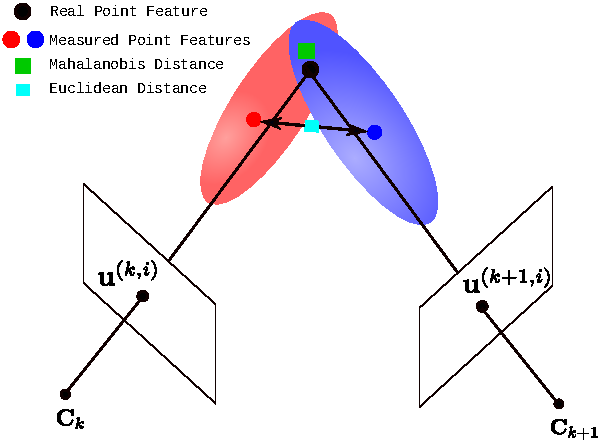
\includegraphics[width=0.9\linewidth,natwidth=640,natheight=640]
{fig/drawings/feature_uncertainty.pdf} \caption[Pose Estimation With Feature
Uncertainty] {When matched image features are back-projected onto the camera
coordinate system, they are supposed to overlap. In practice, they are located
at different positions due to the noise. This effect is illustrated with red
and blue points, both of which refers to the black point that is the real
position of the measured point feature. In the absence of an uncertainty model
of these point features, one can only minimize the Euclidean error distance,
which degrades pose estimation accuracy. Conversely, one can model the point
feature uncertainty with the conic ray model and minimize the Mahalanobis
distance. This is the method we utilize in our VO.} \label{fig:min_mahalanobis}
\end{figure}

With being said, we can now extend the residuals function of our optimization
problem by adding forward-transform.  Let's define the auxilary function in the
following form:

\begin{equation} \mathbf{r_{f}}^{(i)}(\mathbf{x}_{k,k+1}) =
\mathbf{X}^{(i)}_{k+1} - f_f(\mathbf{x}_{k,k+1}, \mathbf{X}^{(i)}_{k})
\end{equation}

where the forward-transform function is defined as:

\begin{equation} f_f(\mathbf{x}_{k,k+1}, \mathbf{X}^{(i)}_{k}) =
\mathbf{q}_{k,k+1}^* \otimes (\mathbf{X}^{(i)}_{k} - \mathbf{t}_{k,k+1})
\otimes \mathbf{q}_{k,k+1} \end{equation}

Now we can reformulate our optimization problem by adding forward and
back-transformation to each other along with corresponding covariance matrices:

\begin{equation} \label{eq:residuals_w_back_and_forward} \mathbf{x^*}_{k,k+1} =
\argmin_{\mathbf{x}_{k,k+1}} \sum_i
||\mathbf{r_b}^{(i)}(\mathbf{x}_{k,k+1})||^2_{\mathbf{Q}^{(i)}_{\mathbf{xyz},k+1}}+
||\mathbf{r_f}^{(i)}(\mathbf{x}_{k,k+1})
||^2_{\mathbf{Q}^{(i)}_{\mathbf{xyz},k}} \end{equation}

With the new auxiliary function, we can minimize the error on both forward- and
back-transformation.  In this way, we include noise occurring in both images
into the optimization process. This technique is taken from
[\cite{RichardHartley2003}, p.101] and is called \textit{error in both images}.
Furthermore, we expand the technique, whose original version is to minimize the
Euclidean error distance, to minimize \textit{Mahalanobis} error distance by
including feature covariances (see figure \ref{fig:min_mahalanobis}).

Let's reformulate the residuals functions in the form of a matrix to simplify
the notation for the optimization problem.  Hence, a single back-transformation
operation for a single feature match is a $\mathbf{r_b}^{(i)}$ single residual
block function.  The same definition applies for the forward-transformation
with $\mathbf{r_f}^{(i)}$.  Note that we only use $\frac{1}{2}$ in front of the
residuals function for cosmetics reasons as it does not effect convergence of
the optimization process.  Here, we reorginize the residual blocks by stacking
residual blocks by columns:

\begin{equation} \begin{aligned} \mathbf{x}^*_{k,k+1} :=
\argmin_{\mathbf{x}_{k,k+1}} \frac{1}{2} \begin{Vmatrix}
\mathbf{r_b}^{(1)}(\mathbf{x}_{k,k+1}) \\
\mathbf{r_f}^{(1)}(\mathbf{x}_{k,k+1}) \\ \vdots \\
\mathbf{r_b}^{(m)}(\mathbf{x}_{k,k+1}) \\
\mathbf{r_f}^{(m)}(\mathbf{x}_{k,k+1})
\end{Vmatrix}^2_{\mathbf{Q}_{\mathbf{xyz},k},\mathbf{Q}_{\mathbf{xyz},k+1}} \\
\end{aligned} \end{equation}

Above equation is the final residuals function that we are going to minimize.
The LM algorithm can be used for the optimization. I refer readers for the
fundamental theory behind the LM algorithm to appendices
\ref{sc_least_squares}.  However, we also need to extend regular least squares
problem to weighted least squares problem since we multiply residual blocks
with inverse covariance matrices.  Let's omit $(k,k+1)$ part and generalize the
problem for convenience:

\begin{equation} \begin{aligned} \mathbf{x}^* = \argmin_{\mathbf{x}}
F(\mathbf{x}) & = \argmin_{\mathbf{x}} \frac{1}{2}
||\mathbf{r}(\mathbf{x})||^2_{\mathbf{Q}} \\ & = \frac{1}{2}
\mathbf{r}(\mathbf{x})^T \mathbf{Q_{xyz}}^{-1} \mathbf{r}(\mathbf{x}) \\ & =
\frac{1}{2} \mathbf{r}(\mathbf{x})^T \mathbf{\Omega}_{\mathbf{xyz}}
\mathbf{r}(\mathbf{x}) \end{aligned}
\end{equation}\label{eq:residuals_objective}

where $\mathbf{\Omega_{xyz} = Q^{-1}_{xyz}}$ is the \textit{information
matrix}, repsesent a relationship between covariance matrices and weighting
process.  That is, the smaller covariance (smaller the uncertainty in other
words) for features, the greater weight will have in the optimization.  In this
respect, the LM will attempt to converge to an optimal solution in which the
rotation and translation information is sufficient by iteratively updating the
state vector:

\begin{equation} \mathbf{x}^{n+1} = \mathbf{x}^{n} \boxplus \Delta \mathbf{x}
\end{equation}

where $\boxplus$ refers to a manifold operation.  The translational part of the
state vector is in Euclidean space. Thus, one can update the state vector with
a regular vector addition operation.  However, this addition operation does not
produce good results for the rotational part. This is because the rotation is
the tangent space.  For the further details of the optimization on a manifold
for our VO, I refer readers to appendices \ref{sc_lsq_manifold}.

To sum up, we explained how we form the residuals function for the optimization
by including back-transform and forward-transform function. We also extended
the regular least squares to weighted least squares problem by incorporating
the feature covariances. In the following section, we will describe how to
propagate the pose covariances.


\section{Covariance of the Estimated Pose} \label{sc_covariance_estim} 

Another important question one can ask in any odometry applications is that
what is the uncertainty, namely covariance, of the odometry measurements?
Generally, traditional VO algorithms do not provide an answer to this question
since it does not take the uncertainty of the features into account.  This
issue introduces a big drawback, especially in sensor applications.  However,
we are now able to estimate a covariance matrix of the estimated pose since we
use the conic ray to model feature uncertainties.  With the help of each pose
covariance, we can represent the possible accumulated covariances along the
trajectory with $3\sigma$ ellipsoids if the relative poses are concatenated as
seen in figure \ref{fig:pose_uncertainty}. 

The fact that we use a metric uncertainty model to represent 3D point features'
noise enables us to estimate a metric pose uncertainty. This property will
produce more accurate pose covariance matrices.  For example, if we had only
detected 3D point feature matches positioned far from Kinect, the pose
covariance would get larger compared to the situation where the features are
placed close to Kinect.  Another determinant is the number of detected feature
matches. Having an insufficient number of features would increase the
covariance as well.  All of these will contribute to the robustness of sensor
fusion applications.  Now that we discuss the importance of having such a
dynamic uncertainty estimation, we will provide the formulation for estimating
the pose covariance matrix in the following part. 

\begin{figure}[H] \centering
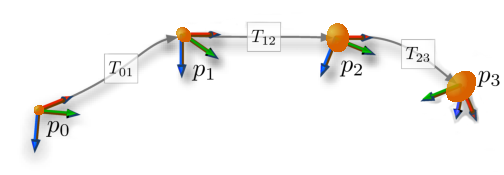
\includegraphics[width=0.7\linewidth,natwidth=640,natheight=640]
{fig/drawings/pose_uncertainty.pdf} \caption[Pose Uncertainty]{This is an
illustration to ellipsoids for pose uncertainties that are growing with every
relative pose estimations. In the absence of absolute sensors that measure the
priori-known landmarks, the pose drift will grow forever.}
\label{fig:pose_uncertainty} \end{figure}

Calculating covarinace matrix for the estimated state vector parameters is
fairly straightforward if the optimization for the relative camera pose is
performed as described in the previous section. We can simply utilize the
\textit{error propagation law}, which I refer readers for to appendices
\ref{sc_error_prop_law} for further details of the theory.  In this case, we
require the Jacobian matrix at the optimal solution and corresponding
covariance  matrices for each point feature. Then, we can propagate them to get
the covariance for the estimated parameters by applying the following equation:

\begin{equation}\label{eq:cov_tq_prop} \mathbf{Q}_{\mathbf{tq},k,k+1} =
(\frac{1}{2})^2 \cdot \mathbf{J'}(\mathbf{x^*}_{k,k+1})^T
\mathbf{Q}_{\mathbf{xyz},k,k+1} \mathbf{J'}(\mathbf{x^*}_{k,k+1})
\end{equation}

where $\mathbf{J'}(\mathbf{x^*}_{k,k+1}) \in \R^{6mx6}$ is the Jacobian of
extended residuals function with backward-, forward-transformation and manifold
in \ref{eq:new_jacobian_chain_rule},

\begin{equation} \begin{aligned} & \mathbf{Q}_{\mathbf{xyz},k,k+1}  =
\begin{bmatrix} \mathbf{Q}_{\mathbf{xyz},k}^{(1)} & \dots & & &\mathbf{0} \\
\mathbf{0} & \mathbf{Q}_{\mathbf{xyz},k+1}^{(1)} & &\dots & \vdots  \\ \vdots &
& \vdots &  &\\ &  & & \mathbf{Q}_{\mathbf{xyz},k}^{(m)} & \mathbf{0} \\
\mathbf{0} &  & & & \mathbf{Q}_{\mathbf{xyz},k+1}^{(m)} \end{bmatrix} \in
\R^{6mx6m} \end{aligned} \end{equation}

is the covariance matrix that comprised of all covarince matrices for all
matched features from $k^{th}$ and $k+1^{th}$ consecutive frames,

\begin{equation}\label{eq:cov_xyz_prop} \begin{aligned} &
\mathbf{Q}_{\mathbf{xyz},k}^{(i)} = \mathbf{J_{bp}}^T(\mathbf{u}^{(i,k)})
\begin{bmatrix} \sigma_u & 0 & 0 \\ 0 & \sigma_v & 0 \\ 0 & 0 &
(\sigma_z^{(i)}(z, \theta))^2 \end{bmatrix} \mathbf{J_{bp}}(\mathbf{u}^{(i,k)})
\in \R^{3x3} \end{aligned} \end{equation}

is the covariance matrix for the $i^{th}$ matched feature from $k^{th}$ frame,

\begin{equation} \begin{aligned} & \mathbf{Q}_{\mathbf{tq},k,k+1}  =
\begin{bmatrix} \sigma_{t_x}^2 & 0 & 0 & 0 & 0 & 0 \\ 0 & \sigma_{t_y}^2 & 0 &
0 & 0 & 0 \\ 0 & 0 & \sigma_{t_z}^2 & 0 & 0 & 0 \\ 0 & 0 & 0 & \sigma_{q_x}^2 &
0 & 0 \\ 0 & 0 & 0 & 0 & \sigma_{q_y}^2 & 0 \\ 0 & 0 & 0 & 0 & 0 &
\sigma_{q_z}^2 \end{bmatrix} \in \R^{6x6} \end{aligned} \end{equation}

is the resulting covariance matrix for the estimated state vector parameters.
In other words, we are now able to calculate the uncertainty of the estimated
pose of the camera.

Notice $(\frac{1}{2})^2$ in front of \ref{eq:cov_tq_prop}.  In the original
error propagation law, this does not exist.  It comes from the fact that we use
both the backward- and forward-transformation in residuals function.  To be
more clear, remember that we represented a relative camera motion with both
back and forward transformation to take errors on both $k^{th}$ and $k+1^{th}$
consecutive images into account. This resulted in having two residuals
$\mathbf{r_b}^{(i)}$ and $\mathbf{r_f}^{(i)}$ for one feature match (see
notation \ref{eq:residuals_w_back_and_forward}).  Therefore, we divide by 2 to
average. The reason we square it is because of the covariance.

Finally, let's summarize this chapter.  At first, we provided a literature
background for an error-aware VO. We argued that all the related work being
done did not use feature uncertainty to produce metric pose covariance. With
this motivation, we gave a recipe for building an error-aware VO which we call
CoVO. Then, we explained how we include feature and depth-related noise models
into the optimization process so that we propagate a covariance matrix for the
estimated relative camera pose. In the next chapter, we will evaluate the
proposed CoVO algorithm with simulated and real-world data. 

\chapter{Evaluation} \label{cp_evaluation}
% ***************************CP5-EVALUATION***************************

Computer vision applicatons like VO require many approximations and linearization 
techniques in order to cope with its dynamic nature for the sake of efficiency.
In practice, many corner cases might occur, no matter how 
good such estimation algorithms are modeled. It is therefore critical 
to verify such systems. Considering that 
the proposed error-aware VO algorithm outputs two information: 
relative pose estimation and its covariance estimation, 
this chapter will be mainly built around two following questions 
that I am going ask:

\begin{enumerate}
  \item What is the \textit{accuracy} of relative pose estimations?
  \item How \textit{consistent} do the algorithm estimate 
    covariance of its pose?
\end{enumerate}

In order to tackle with these questions, simulation environment will 
used to validate the model at first. Then, RGB-D datasets will be used 
to test the algorithm in real-worl environment.

\section{Error Metrics}

There are already 
well-established error evaluation methods in literature so I 
am going to follow them in order to better 
understand characteristics of the proposed algorithm.
If we want to apply these methods on our algorithm, we need to have 
the ground truth pose sequences $\mathbf{x}_{1:n} \in SE(3)$ for 
comparing with the estimated pose sequences $\mathbf{x^*}_{1:n} \in SE(3)$. 
In our calculations, we asumme that both pose sequences are
time-synchronized, equally sampled and have the same length $n$.
However, it is important to note that none of these assumptions are hold 
so we need to be aware of the error caused by these issues. 

\subsubsection{Relative Pose Error}

For evaluating the accuracy of a VO algorithm, it is better 
calculate the relative pose error rather than comparing with the 
absolute (whole) estimated trajectory. This is also refered as Relative 
Pose Error (RPE). 
On the other hand, some VO estimate a relative pose by frame-to-frame and 
some VO by keyframes. 
To able to compare all kinds of VO with each other, a fixed time interval 
$\Delta$ is chosen to calculate the local accuracy of the pose estimation. 
In this way, we take local drifts into account to compare both types of VO algorithms.
Thus, we defined RPE at time instance $i$ as follows:

\begin{equation}
  \mathbf{E}_i := 
  (\mathbf{x}_i^{-1} \mathbf{x}_{i+\Delta})^{-1} 
  (\mathbf{x^*}_i^{-1}\mathbf{x^*}_{i+\Delta})
\end{equation}

One can take a mean of all $E_{1:n}$ RPE, but this hides 
the effect of outliers when $n$ is large.
Instead , we calculate Root Mean Error Squared (RMSE) which compresses the 
error with much more information since it takes mean deviation of the error.
%\subsubsection{Root Mean Squared Error of RPE}
RMSE will show how the mean deviation of the error. For doing so,
$m = n - \Delta$ number of RPE are required to be calculated 
among $n$ pose sequences,:

\begin{equation}
  RMSE(\mathbf{E}_{1:n},\Delta) := \sqrt{\frac{1}{m} \sum_{i=1}^{m}||\mathbf{E}_i||^2}
\end{equation}

Then, we take a mean of all RMSE over whole trajectory:

\begin{equation}
  RMSE(\mathbf{E}_{1:n}) :=  \frac{1}{n} \sum_{\Delta=1}^{n}RMSE(\mathbf{E}_{1:n},\Delta)
\end{equation}

It is important to note that we take $\Delta=1$ when we want to know 
a drift per frame. This is useful when comparing simulation results with 
real world experiments for the same algorithm. 
Conversely, we take $\Delta=30$ when comparing 
the proposed algorithm other VO. This corresponds to a drift per approximately 
1 second.

\subsubsection{Normalized Estimation Error Squared}

The main focus of this thesis is to provide metric uncertainty of the relative 
pose. We do this by propogating the uncertainty of the 3D features points 
through the error model. In this case, it is critical to assess 
consistency of estimated convariance values in order to use it safely in 
filter-based or graph-based sensor fusion applications. 
One of the good metrics to evaluate consistency is 
to calculate Normalized Estimation Error Squared (NEES). This method measures 
the credibility of the provided covariance and it helps us to decide whether 
the predicted uncertainty values are optimisic or pessimistic.
One can calculate NEES if $\mathbf{x}_i$ real pose, $\hat{\mathbf{x}_i}$ predicted 
pose and $\Omega_i = \mathbf{Q}_i^{-1}$ information matrix are known at time 
instance $i$:

\begin{equation}
  \epsilon_i = (\mathbf{x}_i - \mathbf{x^*}_i)^T \mathbf{\Omega}_i (\mathbf{x}_i - \mathbf{x^*}_i) 
  = ||\mathbf{e}_i||^2_{\Omega_i}
\end{equation}

%\subsubsection{Average Normalized Estimation Error Squared (ANEES)}

We also take an average of NEES (ANEES) over whole trajectory:

\begin{equation}
  d \hat{\epsilon} =  \frac{1}{n} \sum_{i=1}^{n} \epsilon_i = 
  \frac{1}{n} \sum_{i=1}^{n} ||\mathbf{e}_i||^2_{\Omega_i}
\end{equation}

TODO: find a synonym for 'it is important to note' phrase!

If the system is linear, has degree of freedom $d=1$ and gaussian noise, 
then the expected value 
$\hat{\epsilon}$ is 1. However, in practice, this does not hold. Therefore, 
another metric when deciding on whether the estimator is consistent or not
is to look at the distribution of NEES over trajectory, which is 
distributed as a chi-square $\chi_d^2$ with $d$ degrees of freedom. 
For an estimator with 3 degree of freedom, acceptance region is
$\hat{\epsilon} \in [2.5,3.5]$ 
when significance level $\alpha$ of $\chi_d^2$ 
is chosen 2.5\% and 50 Monte Carlo runs according to [\cite{Shalom2001}, pp.234-235].
It is important to note that 
we did not implement Manto Carlo simulation for our simulation environment. 
We only treat each estimation as an independent event by adding 
random gaussian noise to the measurements. Thus, when evaluating 
consistency of the estimator in simulation, we aim to get 
$\hat{\epsilon_t}=3$ for translation and $\hat{\epsilon_q}=3$
since both have 3 degree of freedom. On the other hand, when testing 
the estimator with real-world data, we only take upper boundary of 
acceptance region $\hat{\epsilon_t} \in [0, 3.5]$ and 
$\hat{\epsilon_q} \in [0, 3.5]$ since it is 
acceptable to have a conservative estimator rather than overconfident one.


\section{Simulation Environment}

Before testing the proposed algorithm, we will validate the relative 
pose estimation and its covariance with the simulated data. To do so, 
we create a 3D simulation environment that consists of a camera pose, 
3D feature points and their confidence ellipsoids. Our test scenario 
will be comprised of the following steps:

\begin{itemize}
  \item 500 3D feature points are created within camera's observable space.
  \item By utilizing the pinhole model, 
    all 3D feature points are projected onto the camera whose initial pose $p_0$ is known.
  \item Projected feature points are stored in the form of 
    $(u_{1:500}^{0}, v_{1:500}^{0},z_{1:500}^{0})$ sensor measurements as you would usually get it from 
      a regular RGB-D camera. 
    \item The camera is transformed (translated and rotated) with a known distance 
      and rotation $\mathbf{x}_{0,1} = [0.6, 0.6, 0.05, -0.183, -0.183, 0, 0.966]$ 
      to its next pose $p_1$. 
    \item The same 3D feature points are projected with respect to the new pose $p_1$ 
      and stored as $(u_{1:500}^{1}, v_{1:500}^{1},z_{1:500}^{1})$.
    \item In order to introduce uncertainty into the system, the gaussian 
      noises are added on both sensor measurements independently
      $(\hat{u}_{i}=u_{i}+\phi_u, 
      \hat{v}_{i}=u_{i}+\phi_v,
    \hat{z}_{i}=z_i+\phi_z)$ where $\phi\sim\mathcal{N}(\mu,\sigma)$:
      \begin{itemize}
          \item The pixel noises are
            assigned to $(\mu_u=0,\sigma_u=8)$ and $(\mu_v=0,\sigma_v=8)$. 
          \item Whereas, 
            mean of depth noise is $\mu_z=0$ and standard deviation is chosen 
            with respect to feature points' distance to the camera.
            $\sigma_z^{(i)} (z,\theta)$. 
            The lateral noise and the surface angle $\theta$ is assumed to be 0.
            The depth's noise model is discussed in \ref{sb_sc_depth_uncertainty}.
        \end{itemize}
    \item For every measurements, convariance matrices 
      $(\mathbf{Q}_{xyz}^{0,1:500}, \mathbf{Q}_{xyz}^{1,1:500})$ are formed with 
      the same standard deviations of the added noises, where  
      $\mathbf{Q_{xyz}}^{(i)} = \mathbf{J_{bp}}(\mathbf{u})^T
  \begin{bmatrix} 
    \sigma_u^2(=8^2) & 0 & 0 \\ 
    0 & \sigma_v^2(=8^2) & 0 \\
    0 & 0 & (\sigma_z^{(i)}(z, \theta))^2
  \end{bmatrix} \mathbf{J_{bp}}(\mathbf{u})$.

    \item Perfectly matched noisy 3D feature point pairs along with their covariances 
      are given to the optimizer that is discussed in \ref{sc_rel_pose_est_w_uncertainty} 
      to estimate $\mathbf{x^*}_{0,1}$ and $\mathbf{Q}_{\mathbf{t,q}}^{0,1}$.
    \item This whole process is repeated 1000 times.
\end{itemize}

In the following simulation figures, we implement discussed scenario into 
a 3D space. In this environment, we have  
noisy 3D feature points, confidence ellipsoids whose center is around the 
noisy feature points and real position of the 3D feature points that are somewhere 
inside the ellipsoids.

% Distribution of Point Clouds in 3D at p0
\begin{figure}[H]
  \centering
  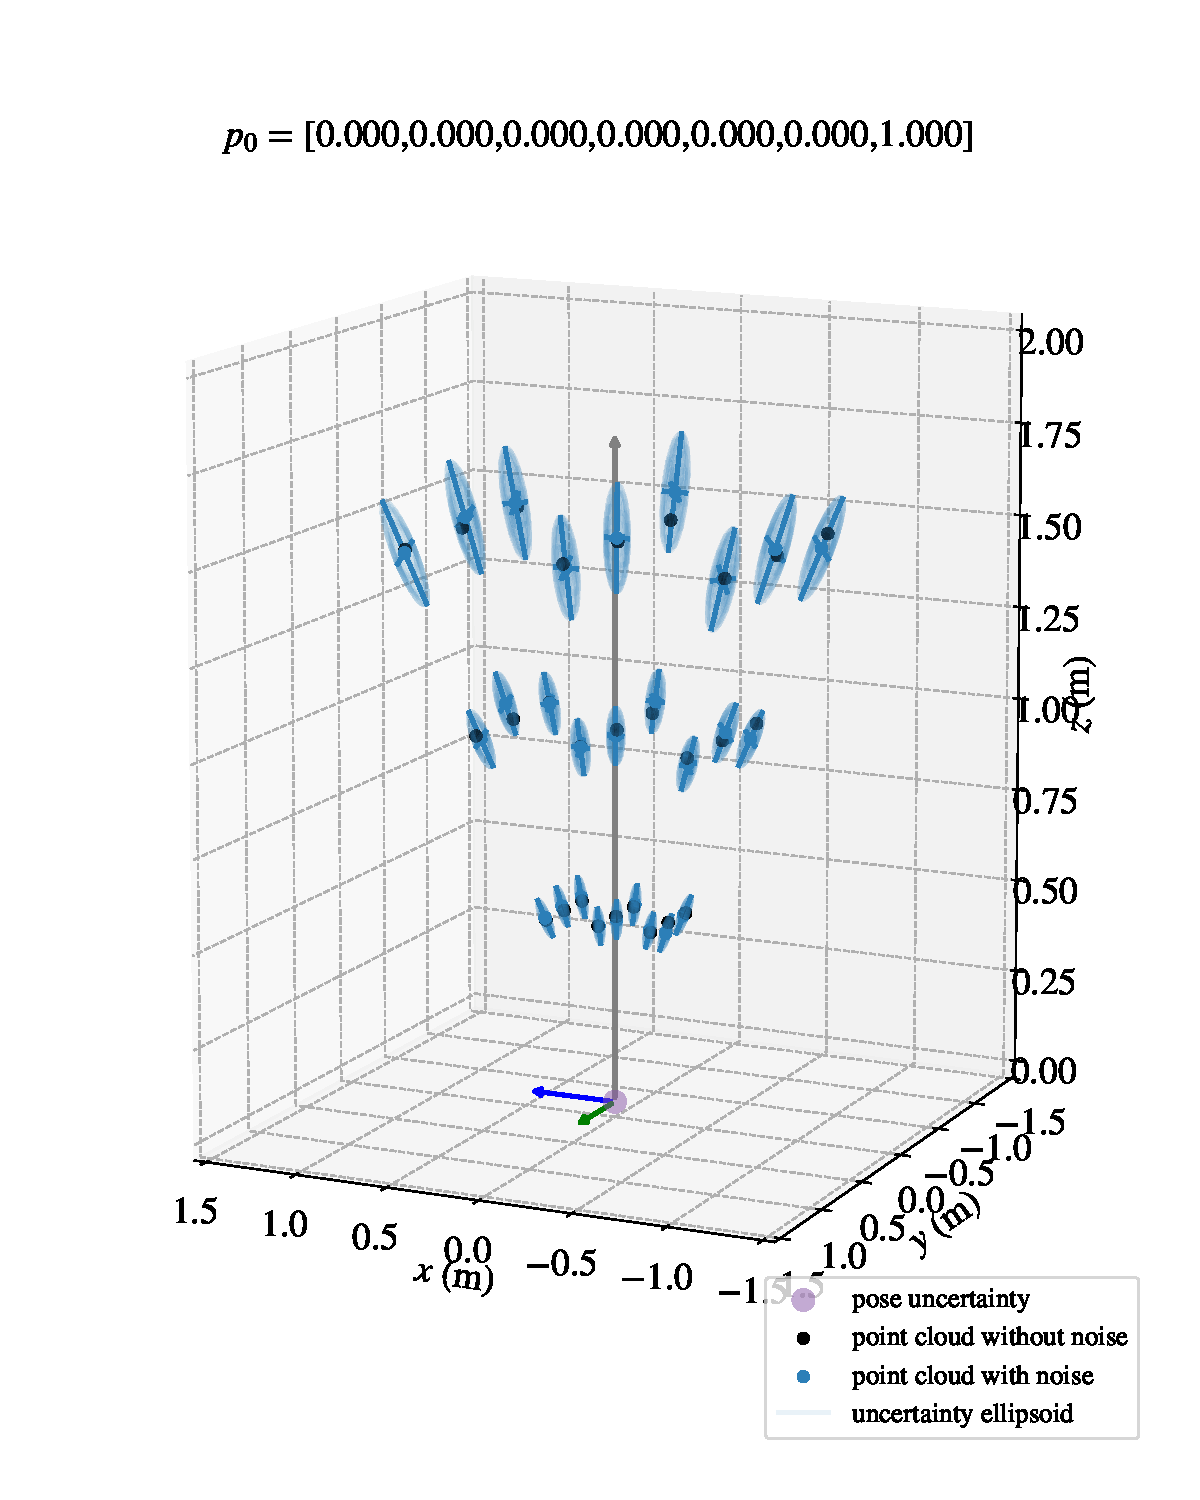
\includegraphics[width=\linewidth,natwidth=640,natheight=640]
  {fig/eva_graphs/sim_at_p0.pdf}
  \caption{asda}
	\label{fig:sim_at_p0}
\end{figure}

The figure \ref{fig:sim_at_p0} depicts the environment at its initial pose $p_0$. 
Note that we only draw small subset of 3D feature points and scaled the 
confidence ellipses by 10 to gain visibility. Notice how 
size and orientation of the confidence ellipsoids are situated according to 
the conic ray model.


% Distribution of Point Clouds in 3D at p1
\begin{figure}[H]
  \centering
  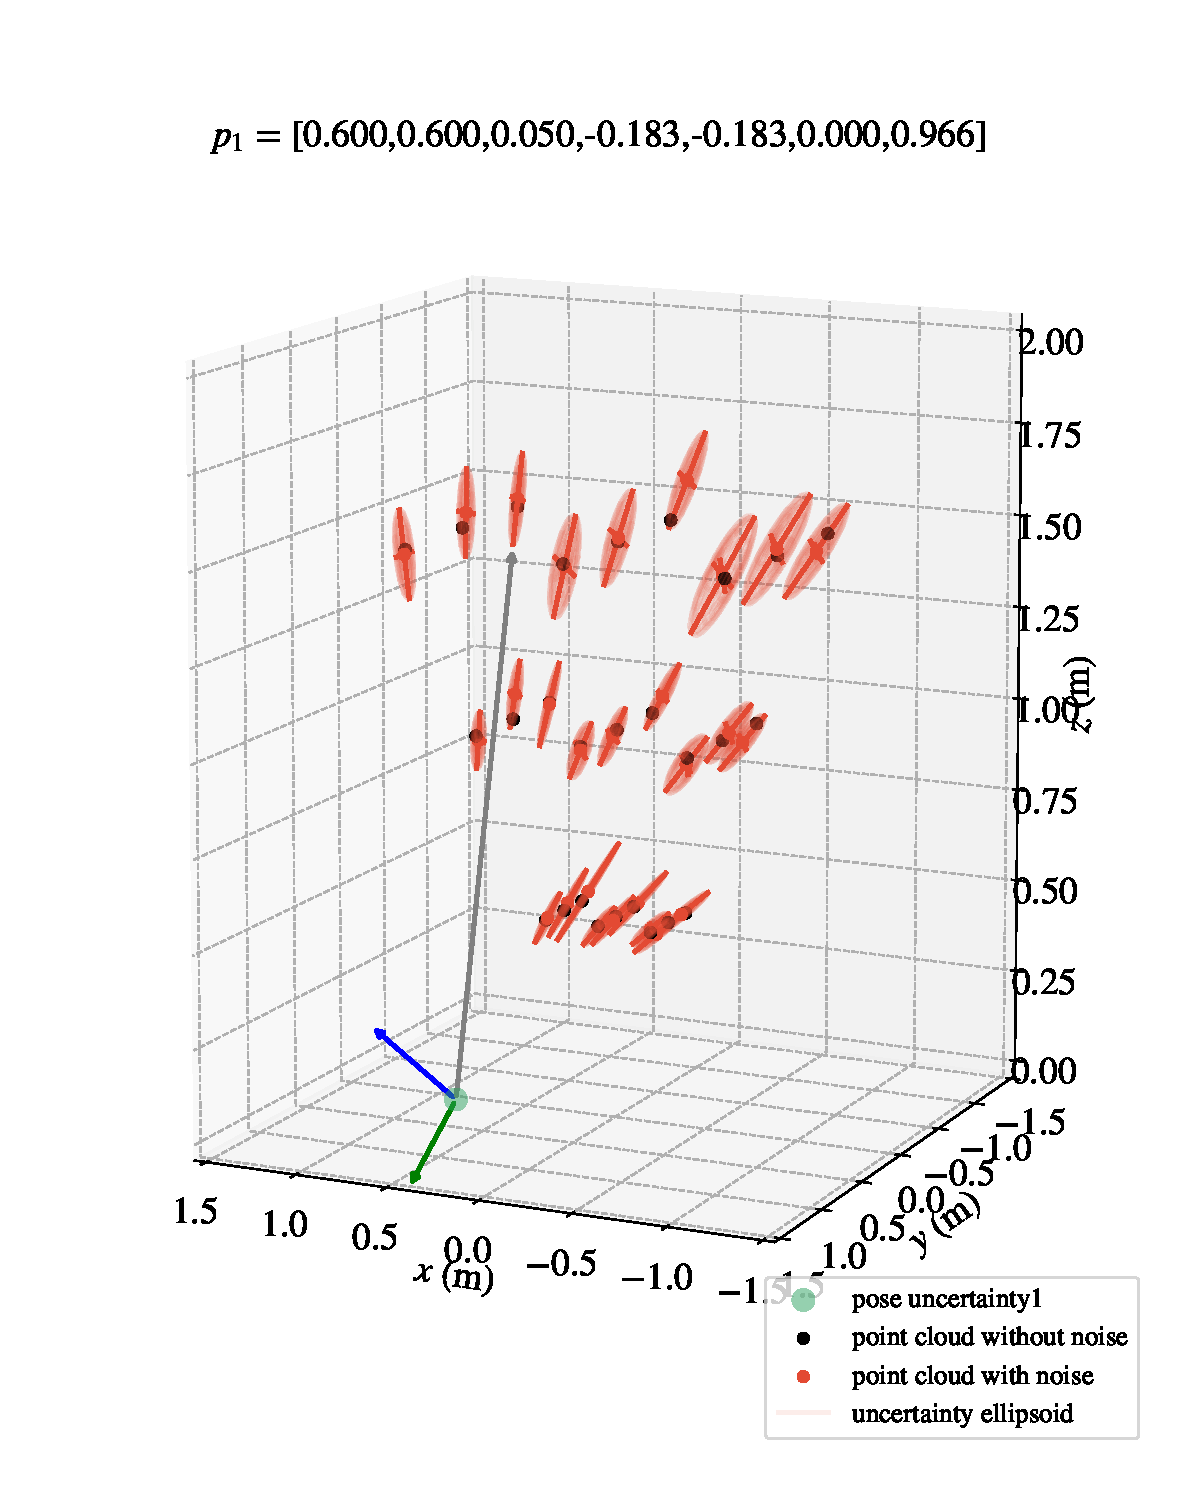
\includegraphics[width=\linewidth,natwidth=640,natheight=640]
  {fig/eva_graphs/sim_at_p1.pdf}
  \caption{asda}
	\label{fig:sim_at_p1}
\end{figure}

Then, we move and rotate the camera to its next pose $p_1$ in the figure 
\ref{fig:sim_at_p1}. Notice how confidence ellipsoids are changed with 
the new camera pose accordingly.


\begin{figure}[H]
  \centering
  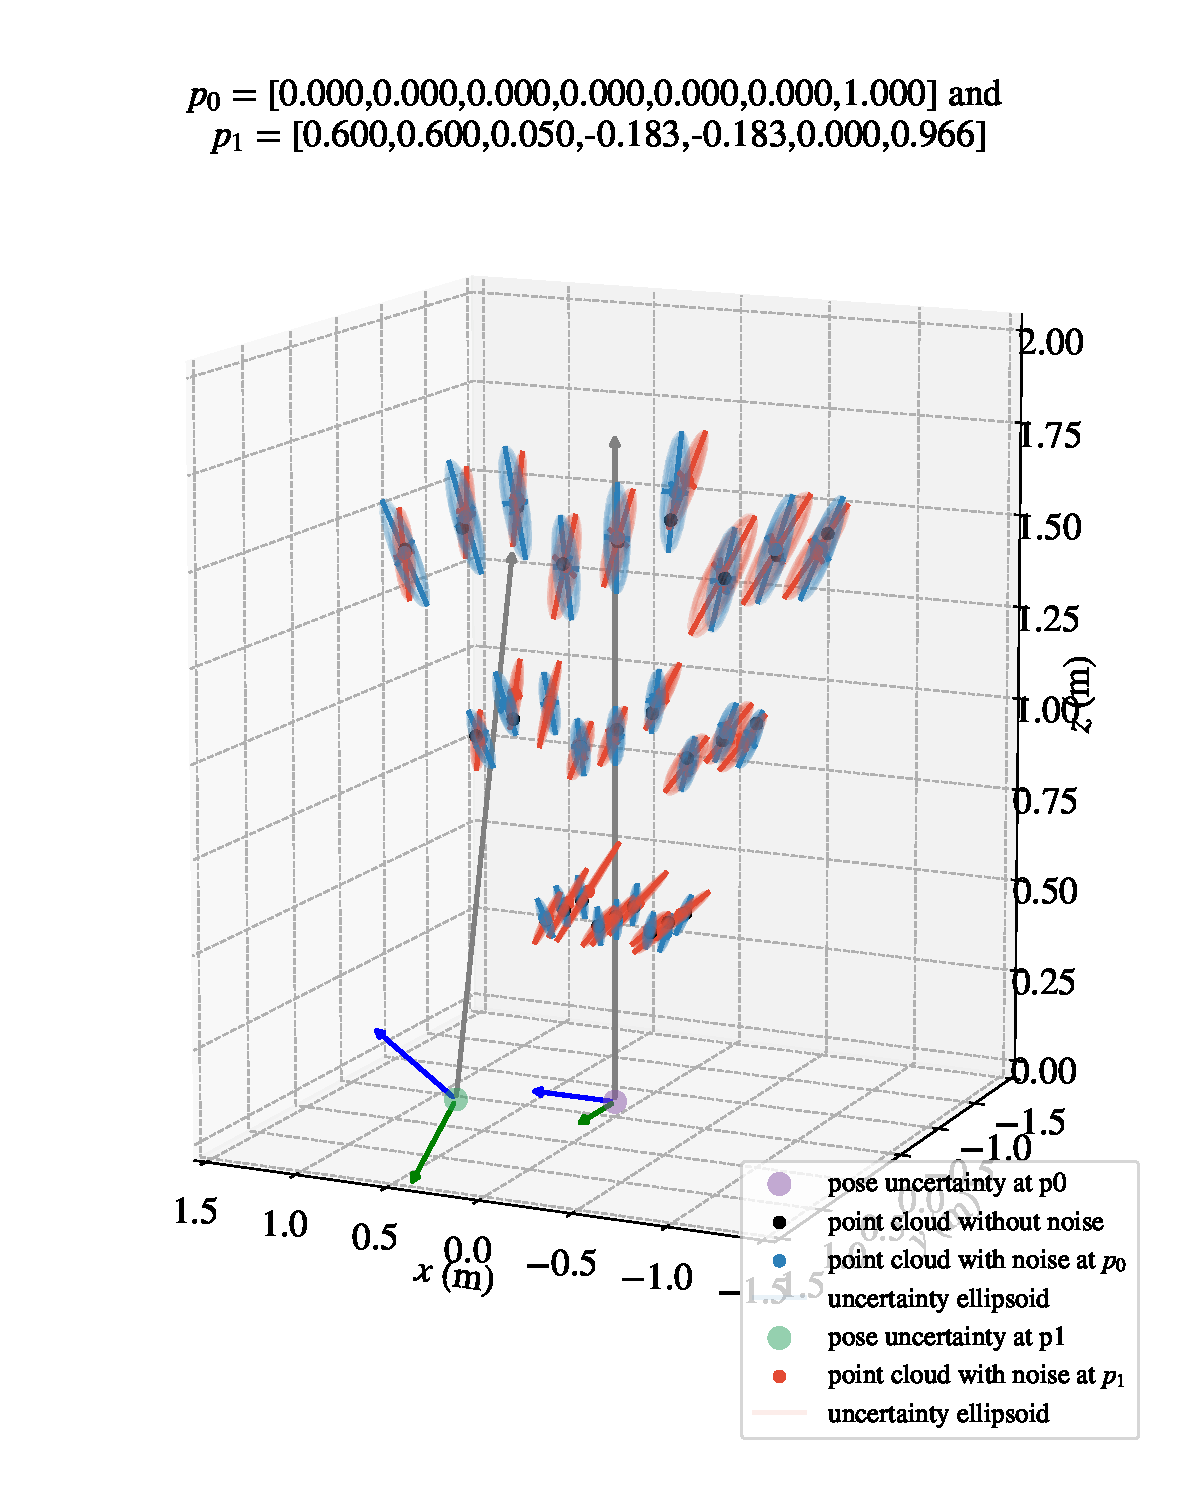
\includegraphics[width=\linewidth,natwidth=640,natheight=640]
  {fig/eva_graphs/sim_at_p0p1.pdf}
  \caption{asda}
	\label{fig:sim_at_p0p1}
\end{figure}

Finally, the figure \ref{fig:sim_at_p0p1} shows how confidence ellipsoids 
from both views intersect each other and include the real feature points within 
the intersected space.

% 4
\subsection{RPE and The Estimated Covariances}

With the simulated data, we estimate relative poses $\mathbf{x^*}_{1:1000}$
and its convariances $\mathbf{x^*}_{1:1000}$. Then, we calculate RPE with 
$\Delta=1$ so that we validate whether the error lies within the 3 sigma bounds
for each parameters of the state vector. 3 sigma bounds corresponds to a rule of 
thumb that expresses 99.7\% probability as near certainty.


% Translation RPE with 3 sigma 
\begin{figure}[H]
  \centering
  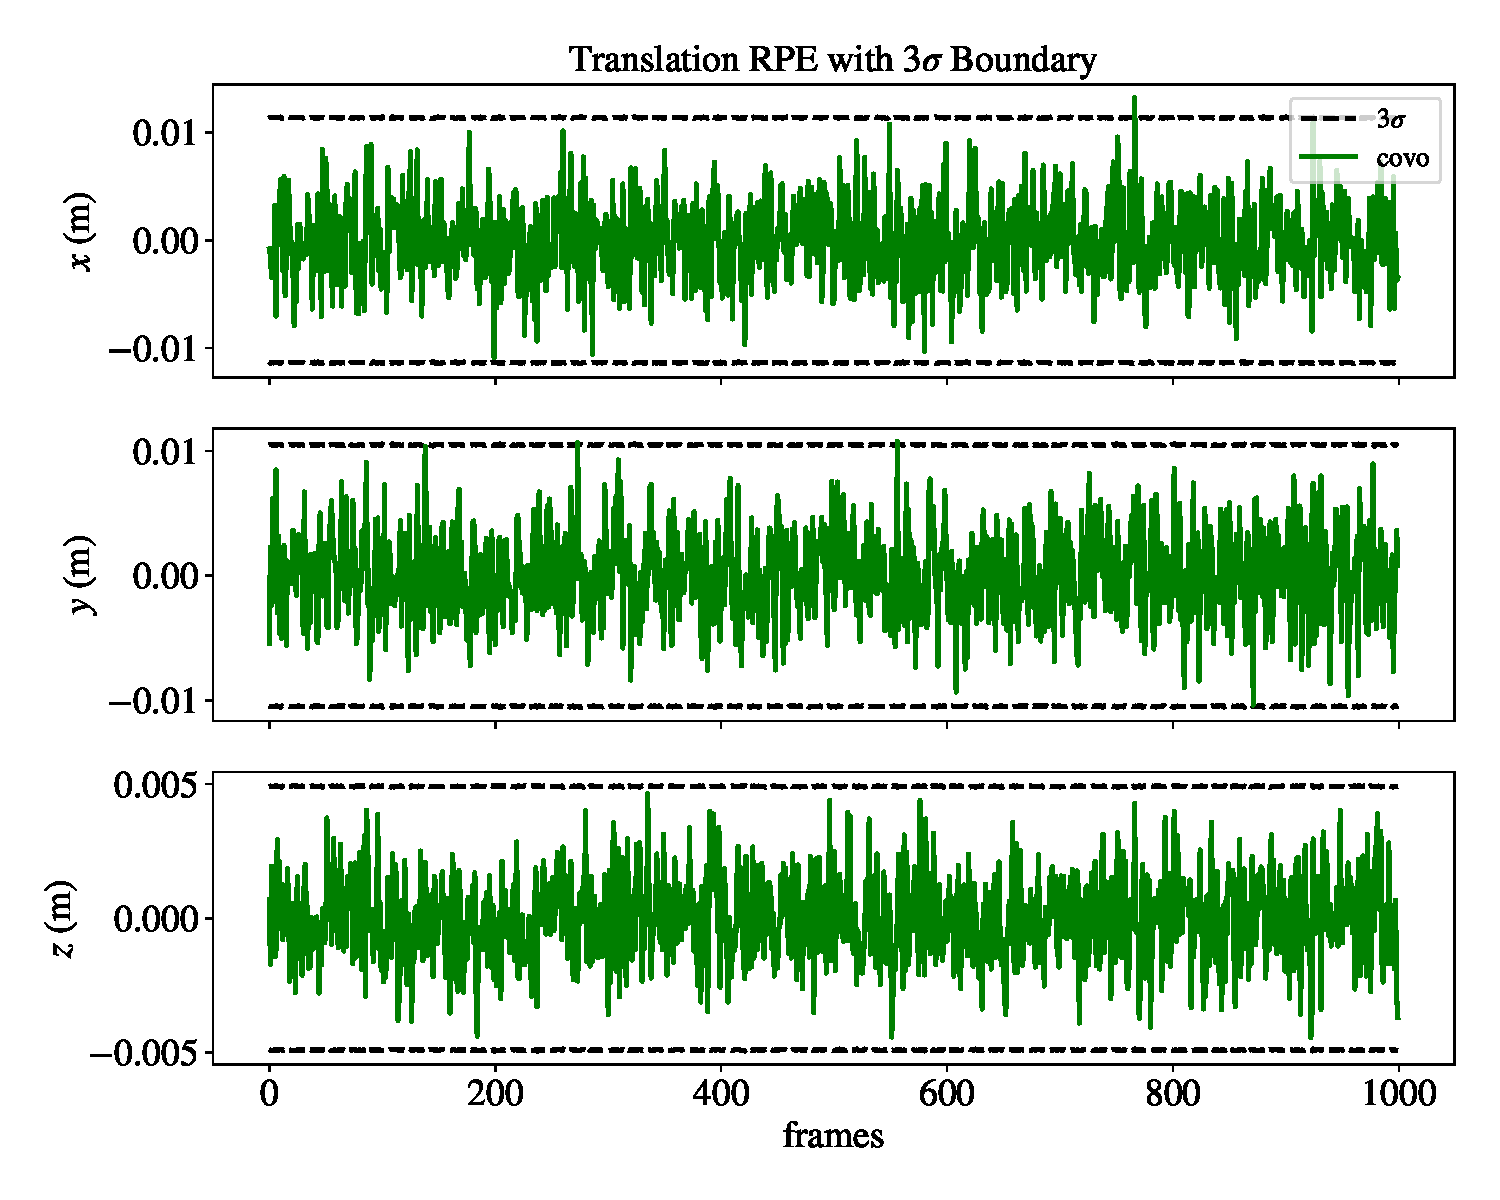
\includegraphics[width=0.8\linewidth,natwidth=640,natheight=640]
  {fig/eva_graphs/synt_trans_rpe_3sigma.pdf}
  \caption{asda}
  \label{fig:synt_trans_rpe_3sigma}
\end{figure}

As seen in figure \ref{fig:synt_trans_rpe_3sigma}, parameters of the translation 
are bounded with 3 sigma with maximum 2 or 3 predictions which is statistically 
acceptable. 

% Rotation RPE with 3 sigma 
\begin{figure}[H]
  \centering
  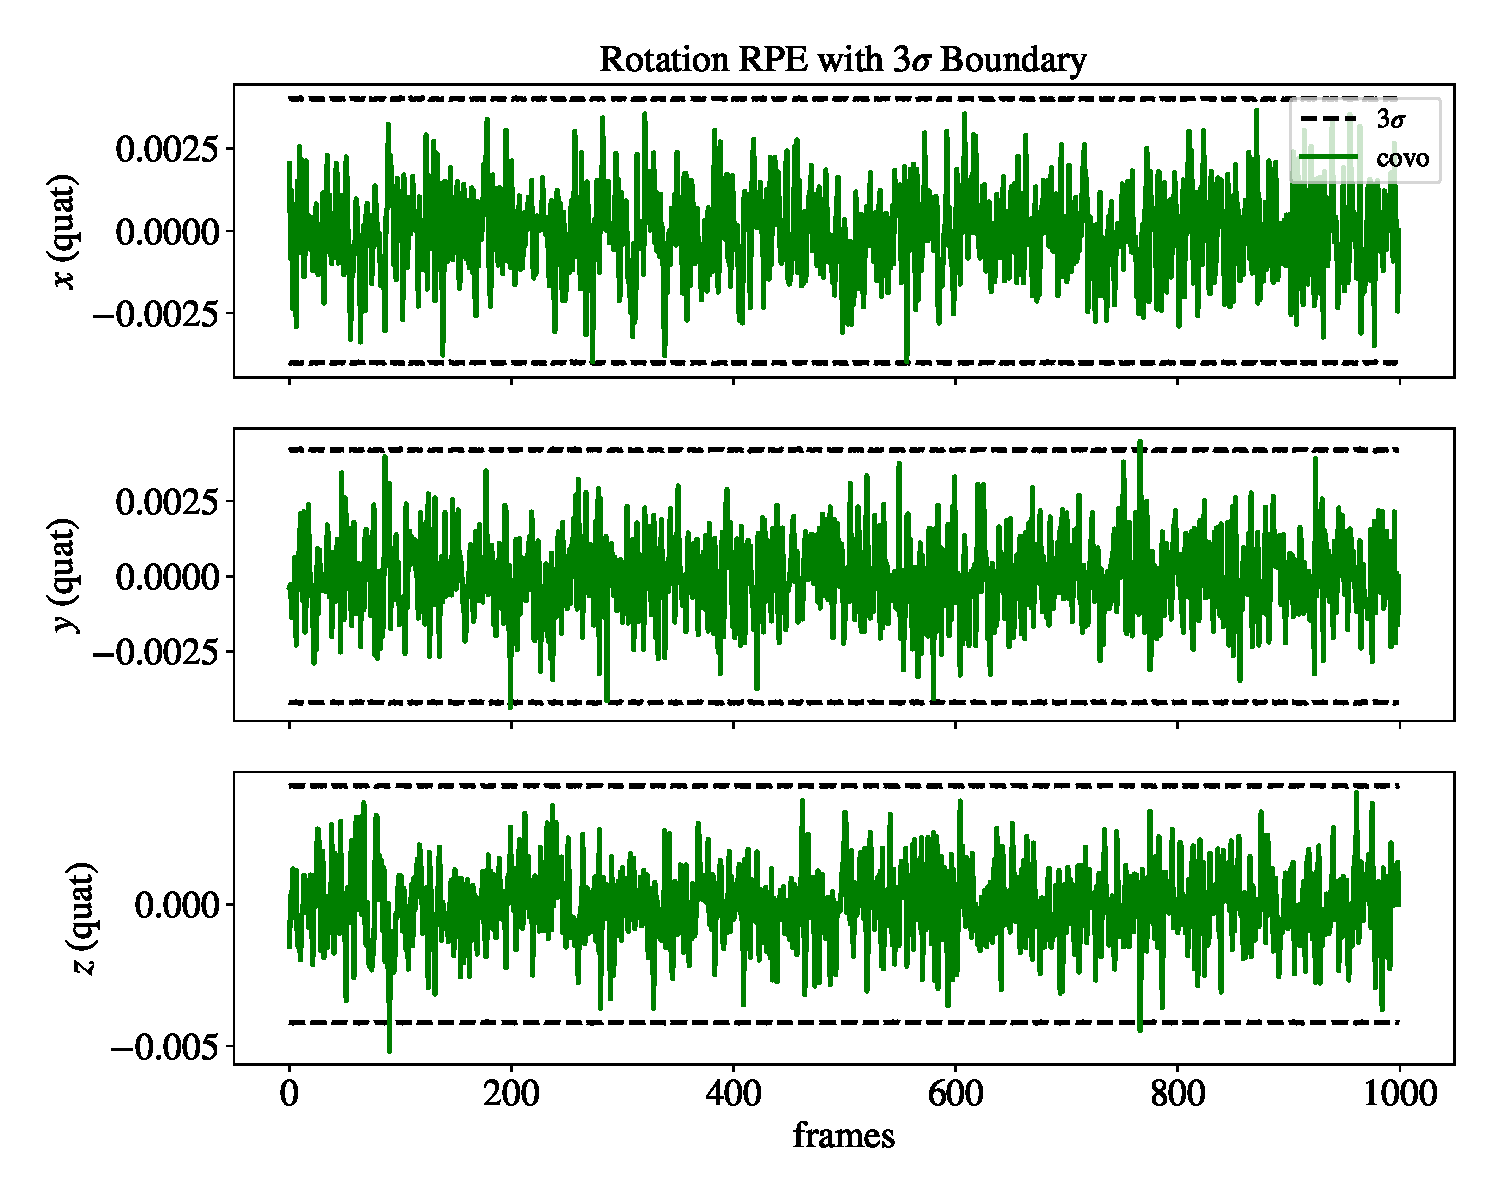
\includegraphics[width=0.8\linewidth,natwidth=640,natheight=640]
  {fig/eva_graphs/synt_rot_rpe_3sigma.pdf}
  \caption{asda}
	\label{fig:2d_local_coords_in_world_coords}
\end{figure}

The same behavior is observed for the rotation as well. This indicates that 
the propagated covariances of the estimated poses based on the 
proposed model produce statistically meaningful uncertainty with simulated data 
if $3\sigma$ bounds are considered. However, $3\sigma$ bounds evaluations itself 
is not enough to prove estimator's credibility. Thus, further evaluations are 
done with NEES.

% 3
\subsection{Evaluation of Estimated Covariances}

Even though $3\sigma$ bounds confirm that our algorithm provides consistent 
pose estimation given RPE is bounded, we need to check whether the 
covariance of the estimated pose are being too optimistic or not.
Hence, we run our simulation as described at the beginning of this section. 
We get ANEES; i.e, 15.64 for translation and 15.72 for rotation. 
We also illustrate the results in figure \ref{fig:test_hist_nees_1}.


\begin{figure}[H]
\begin{tabular}{ccc}
\centering
\subcaptionbox{NEES}{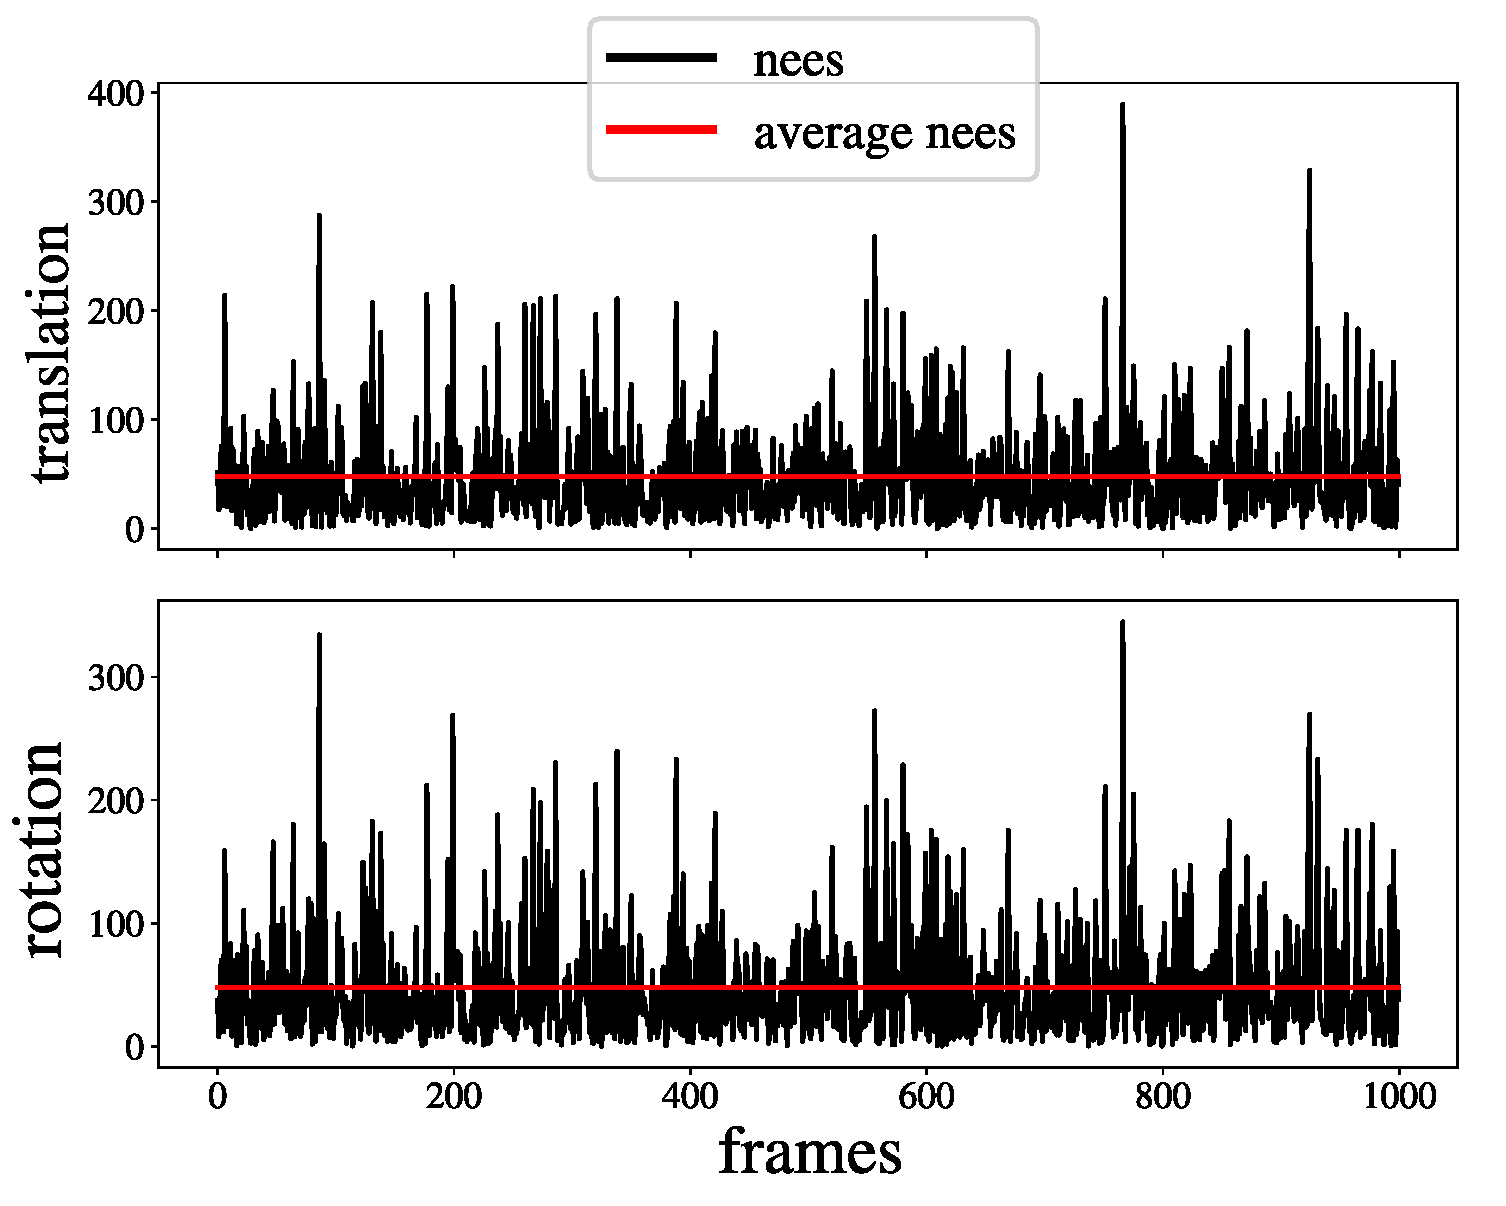
\includegraphics[width = 0.55\linewidth]{fig/eva_graphs/synt_nees.pdf}} &
\subcaptionbox{Histogram of NEES}{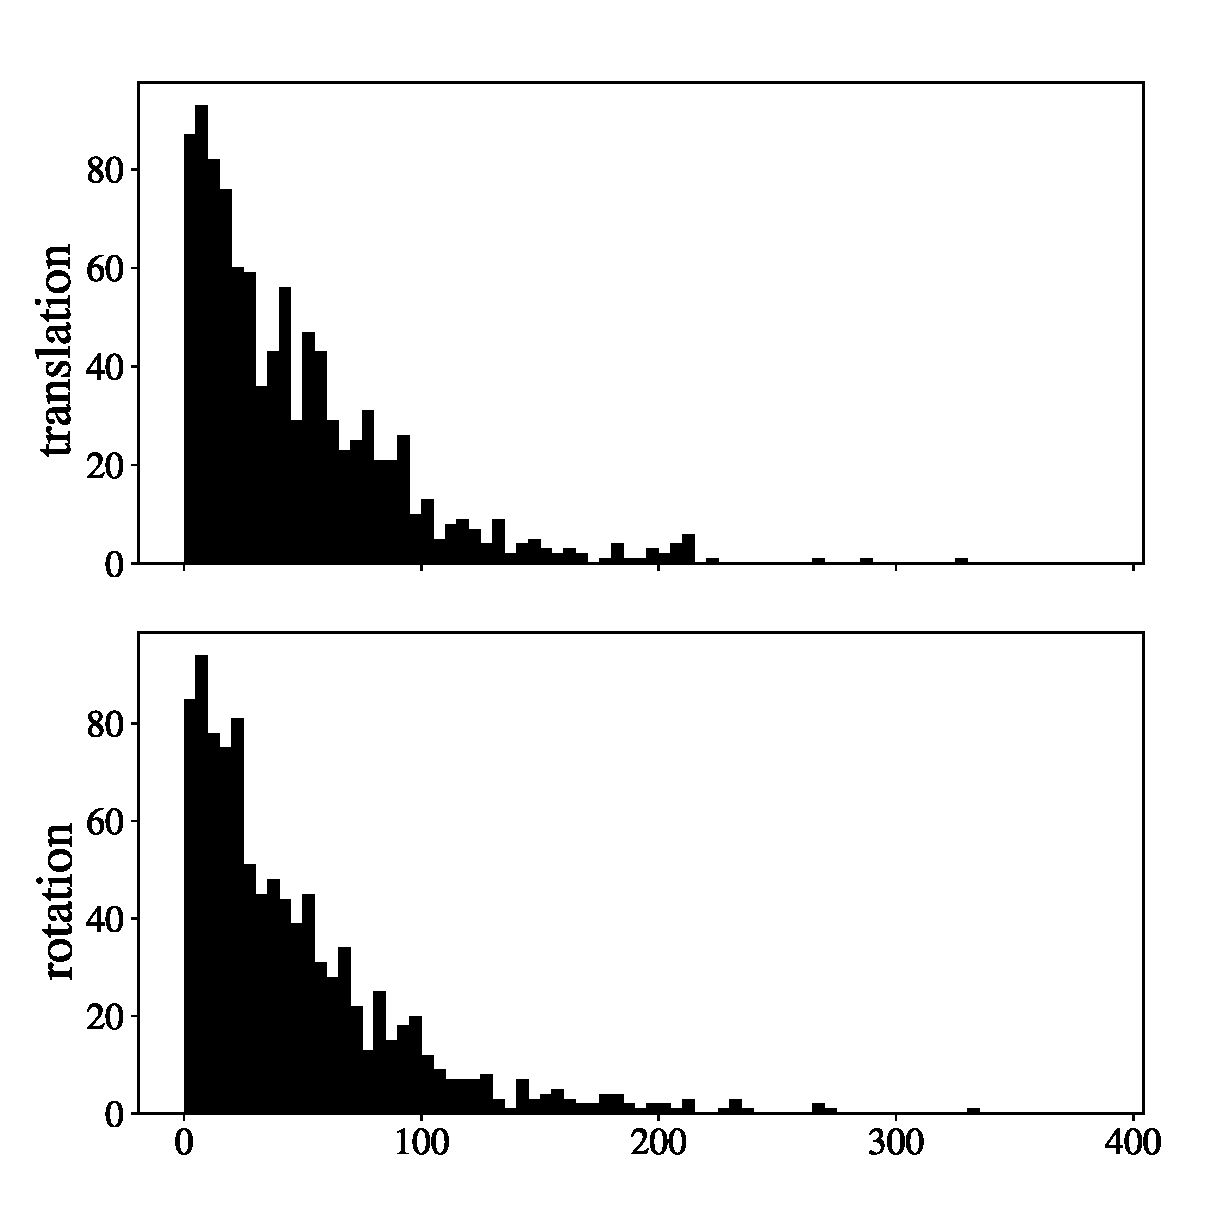
\includegraphics[width = 0.40\linewidth]{fig/eva_graphs/synt_hist_nees.pdf}}
\end{tabular}
\caption{Remove Y axes title and Y axes thick from graphs!!!}
\end{figure}\label{fig:test_hist_nees_1}

%Translation Average NEES: 15.64
%Rotation Average NEES: 15.72

These results show that the estimator is not consistent. This is because 
the projection operation introduces non-linearity to the system and 
we only approximate covariance of 3D feature points with first-order 
taylor expansion. This linearization process does not work well with 
large noises. In this case, [\cite{Shalom2001}, pp.395-397] 
suggests couple of heuristic methods to make the estimator consistent.
Among them, we apply multiplication of estimated covariance $\mathbf{Q_{t,q}}^{(k,k+1)}$
by scaling factor $\phi$ after optimiziton.

\begin{figure}[H]
\begin{tabular}{ccc}
\centering
\subcaptionbox{NEES}{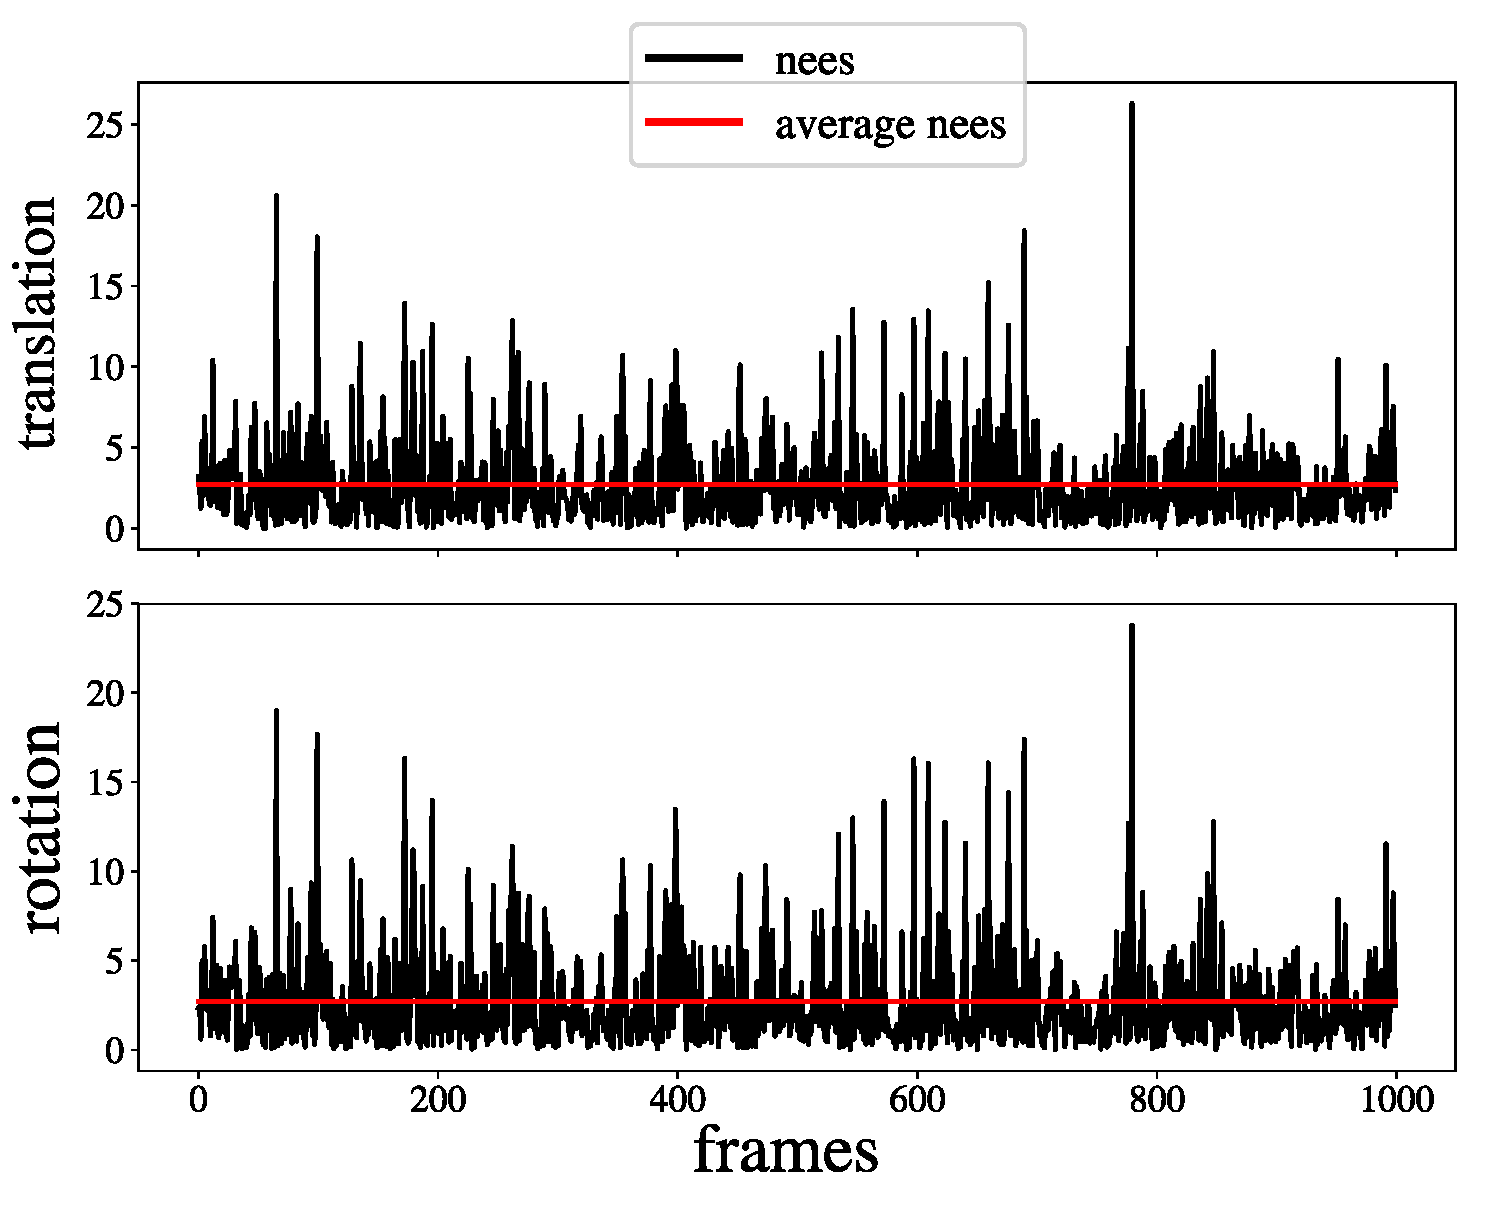
\includegraphics[width = 0.55\linewidth]{fig/eva_graphs/synt_nees_2.pdf}} &
\subcaptionbox{Histogram of NEES}{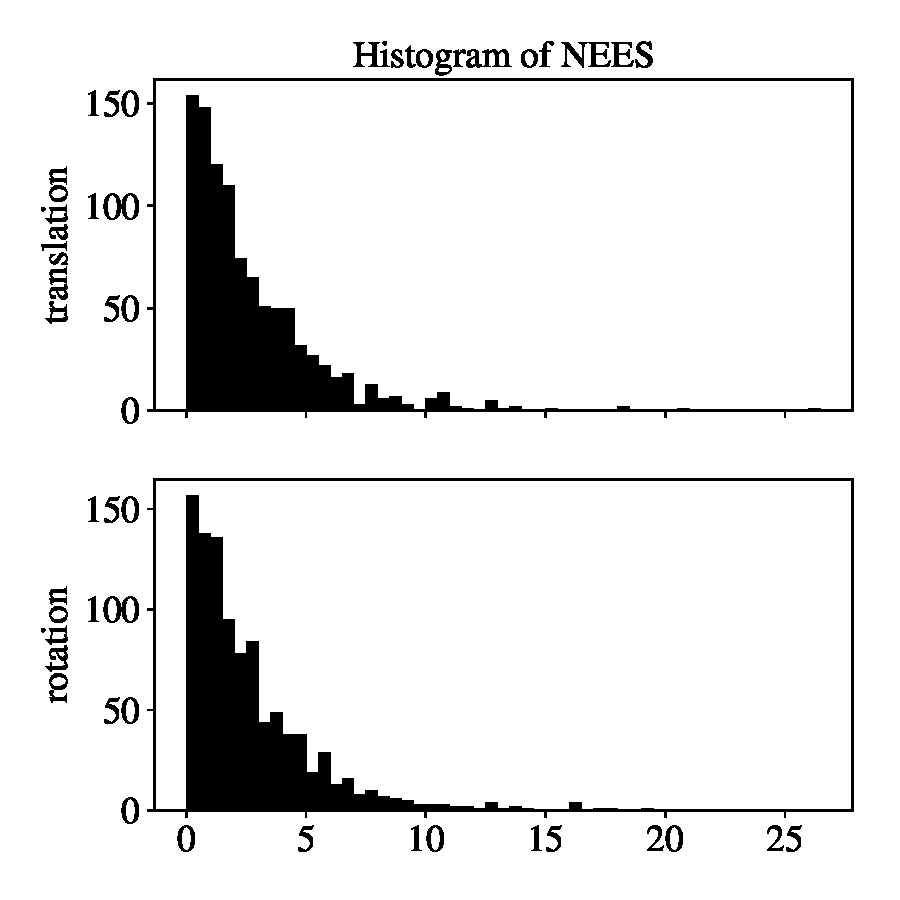
\includegraphics[width = 0.40\linewidth]{fig/eva_graphs/synt_hist_nees_2.pdf}}
\end{tabular}
\caption{Remove Y axes title and Y axes thick from graphs!!!}
\end{figure}\label{fig:test_hist_nees_2}

We find out that ANEES for translation and rotation becomes 2.7 and 2.69, 
respectively when taking $\phi=4^2$ and the results are shown in figure 
\ref{fig:test_hist_nees_2}. These values can be accepted as we consider 
the estimator to be consistent for this setup.

%Translation Average NEES: 2.70
%Rotation Average NEES: 2.69

\section{TUM RGB-D Dataset}

TUM dataset \cite{Sturm2012a} provides an extensive bechmark capability for 
RGB-D based Visual SLAM or VO systems. It consists of datasets that are 
collected in two different indoor environment; i.e, fr1 refers to 
datasets collected in an office $(6\times 6 m^2)$ and fr2 is colleced in an open spaced 
garage $(10\times 12m^2)$. In our experiments, we choose a subset of datasets that are mainly 
suitable for VO and has sufficient texture on the images. 
The selected datasets are given in table \ref{tb:tum_dataset}.
In addition, calibration parameters of RGB and depth images are validated 
by the time-synchronized ground truth measurements recorded by a motion capture system.

\begin{center}
  \begin{tabular}{lccc}
    \hline
    Dataset & Duration & Avg. Trans. & Avg. Rot.\\
     Name & [s] & Vel. [m/s] & Vel. [deg/s]\\
    \hline
    fr1 xyz   & 30 & 0.24 & 8.92\\
    fr1 rpy   & 28 & 0.06 & 50.15\\
    fr1 room  & 49 & 0.33 & 29.88\\
    fr1 360   & 29 & 0.21 & 41.60\\
    fr1 desk  & 23 & 0.41 & 23.33\\
    fr1 desk2 & 25 & 0.43 & 29.31\\
    fr2 desk  & 99 & 0.19 & 6.34\\
    \hline
    \end{tabular}
  \end{center}\label{tb:tum_dataset}

  In the following sections, we will use these datasets to validate 
  our relative pose estimation and its covariance 
  with regards to accuracy and consistency.

\subsection{Discovering the Effect of Pseudo Inliers on Pixel Uncertainty}\label{sc_pseudo_inliers}

As discussed earlier in section \ref{sb_sc_pixel_uncertainty}, pixel 
uncertainty caused by quantization operation is treated as half pixel. 
Nevertheless, this error is itself not sufficient when choosing 
standard deviation of pixel noise for covariance of 3D features 
to be propagated through the \ref{} equation. Remember that 
we still had outliers in feature matching even after applying RANSAC, 
which we call them as pseudo inliers. We proposed to treat them as 
inliers, but they will increase the pixel uncertainty. We also assume that 
RANSAC will bound these pseudo inliers. Thus, we are interested in 
determining the boundaries which we will set them as pixel uncertainties 
We determine them using TUM RGB-D and the ground truth measurements.

% Time-based error histogram with 20 frame discrete window
% - Show that pixel errors are gaussian and stds are different along the path

\begin{figure}[H]
  \makebox[\textwidth][c]{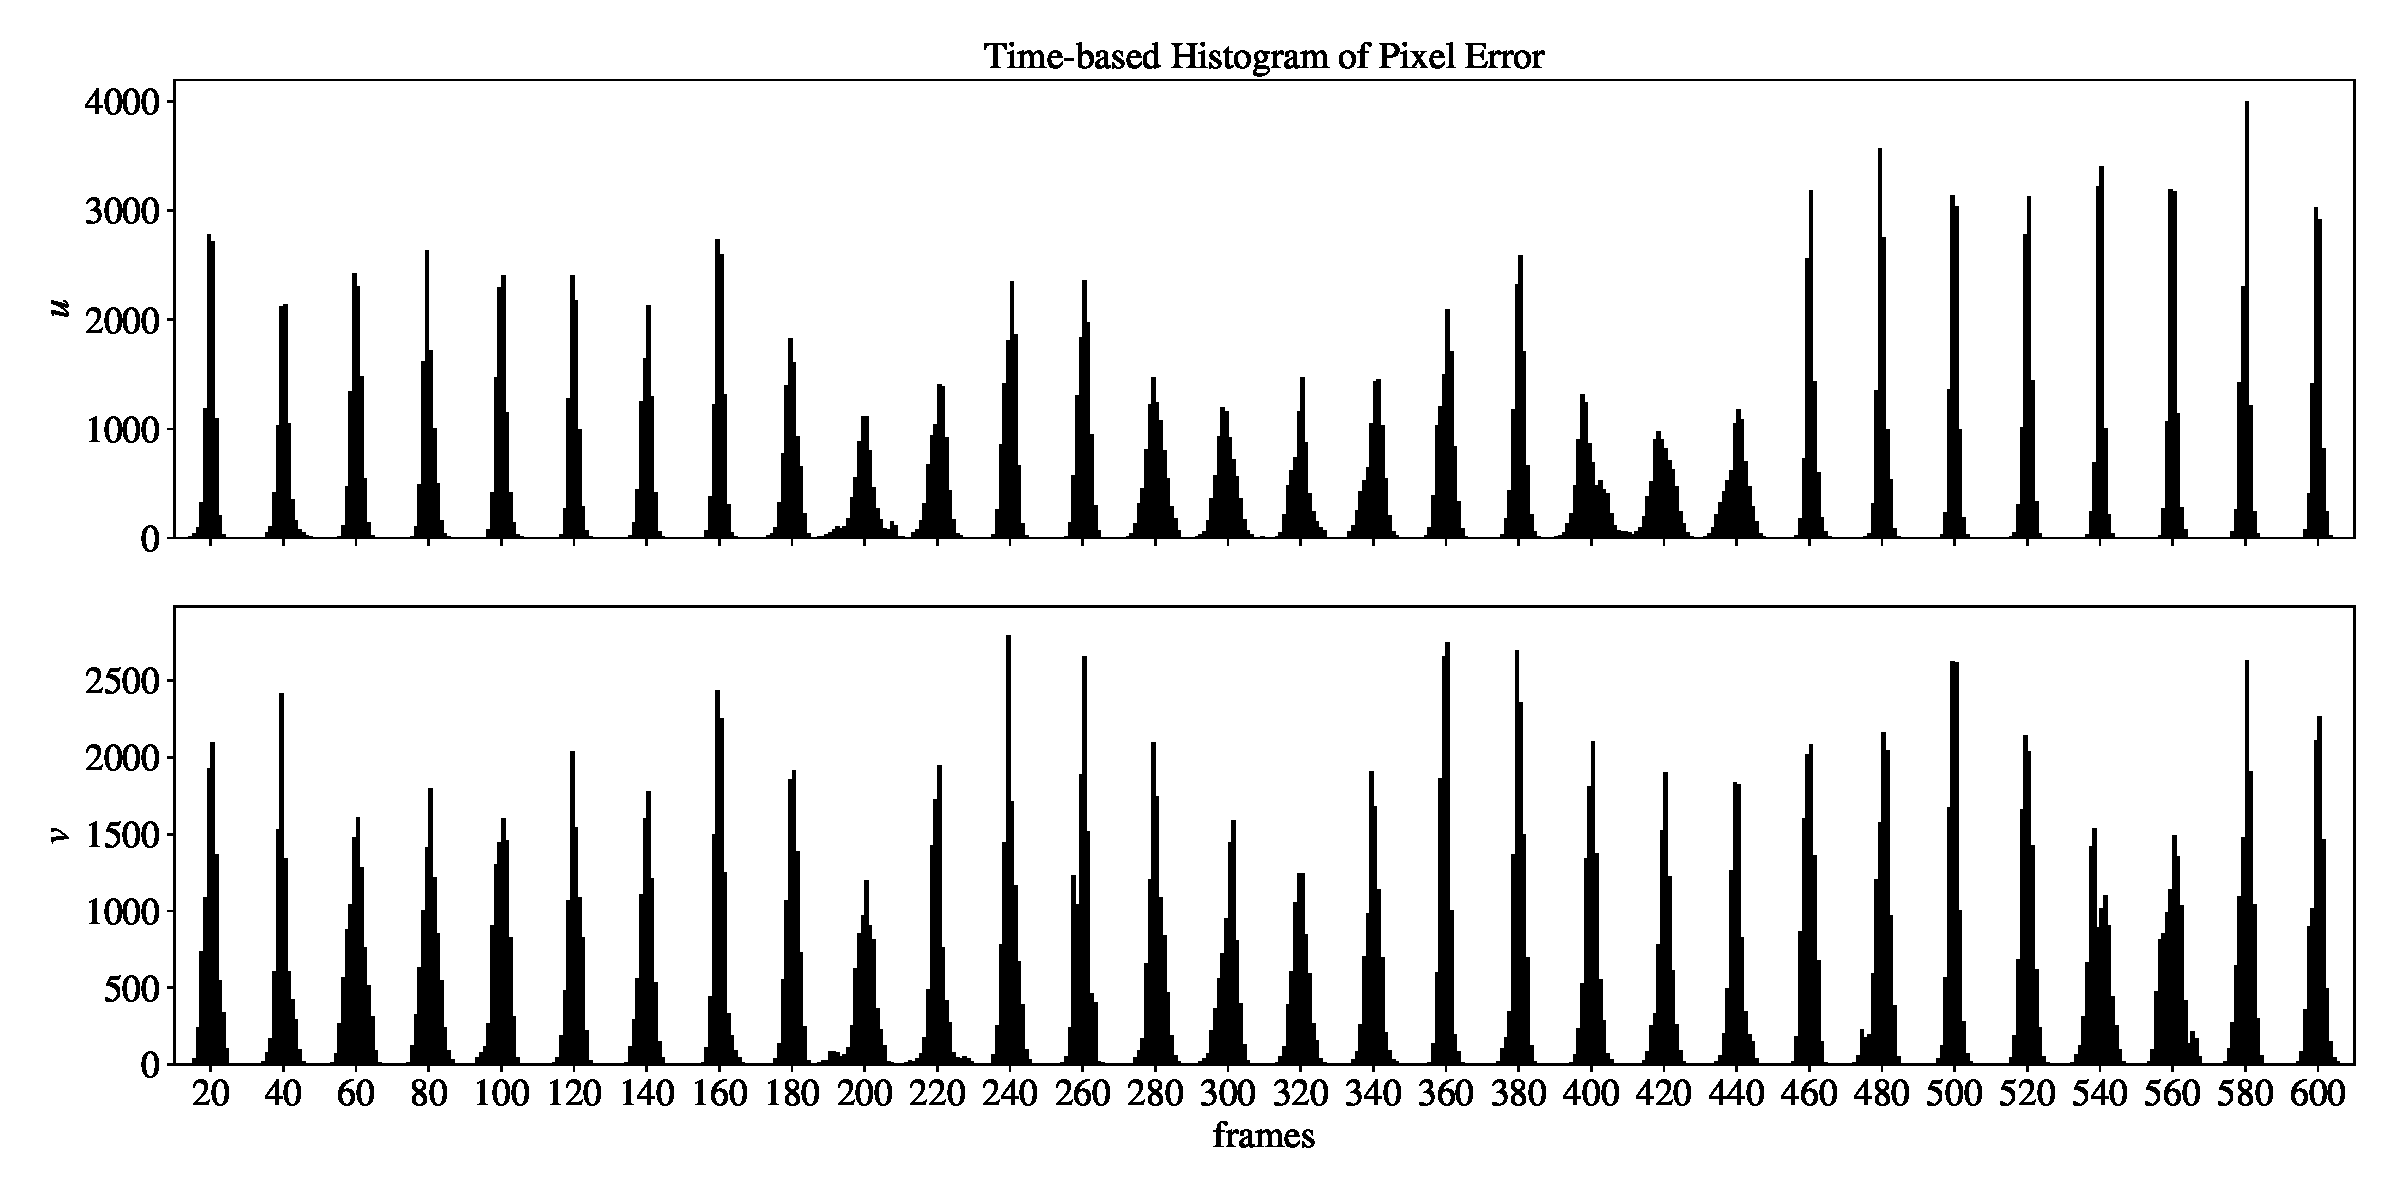
\includegraphics[width=1.4\linewidth,natwidth=640,natheight=640]
  {fig/eva_graphs/tum_fr1_xyz_tbased_hist_uv_err.pdf}}
  \caption{explain the window}
\end{figure}\label{fig:time_based_hist_pix_err}

Let's remind ourselves with the procedures of the pipeline.
To find the pixel error caused by pseudo inliers, we run our VO pipeline 
up until the optimization part estimating the pose. 
To do so, we first extracted features, then matched them and finally filtered outliers with RANSAC. 
At this point, we have feature matches that includes pseudo inliers. 
Now, instead of estimating the relative pose,
we can identify boundaries of the pseudo inliers caused by RANSAC 
by using ground truth data. With using translation and rotation information 
from ground truth, we project features matches one on another. 
Then, for some matches, we expect to get pixel errors to be greater than 1 as 
they are the pseudo inliers.
This test case is applied on every consecutive frame of the whole trajectory.
Next, we illustrate the results in a time-based scheme to observe 
how the pixel error changes throughout the trajectory. The illustration 
gathered by 'fr1 xyz' dataset is given in figure \ref{fig:time_based_hist_pix_err}.
As observed, pixels error mainly caused by pseudo inliers are distibuted as 
gaussian and its standard deviation changes over the trajectory. To 
see how it changes we draw the time-based standard deviation of the pixel errors 
in figure \ref{fig:time_based_std_pix_err}.

TODO: THERE IS SOMETHING WRONG WITH THE NUMBERING OF FIGS.
% Time-based std with 5 frame sliding window with fr1_xyz

\begin{figure}[H]
  \centering
  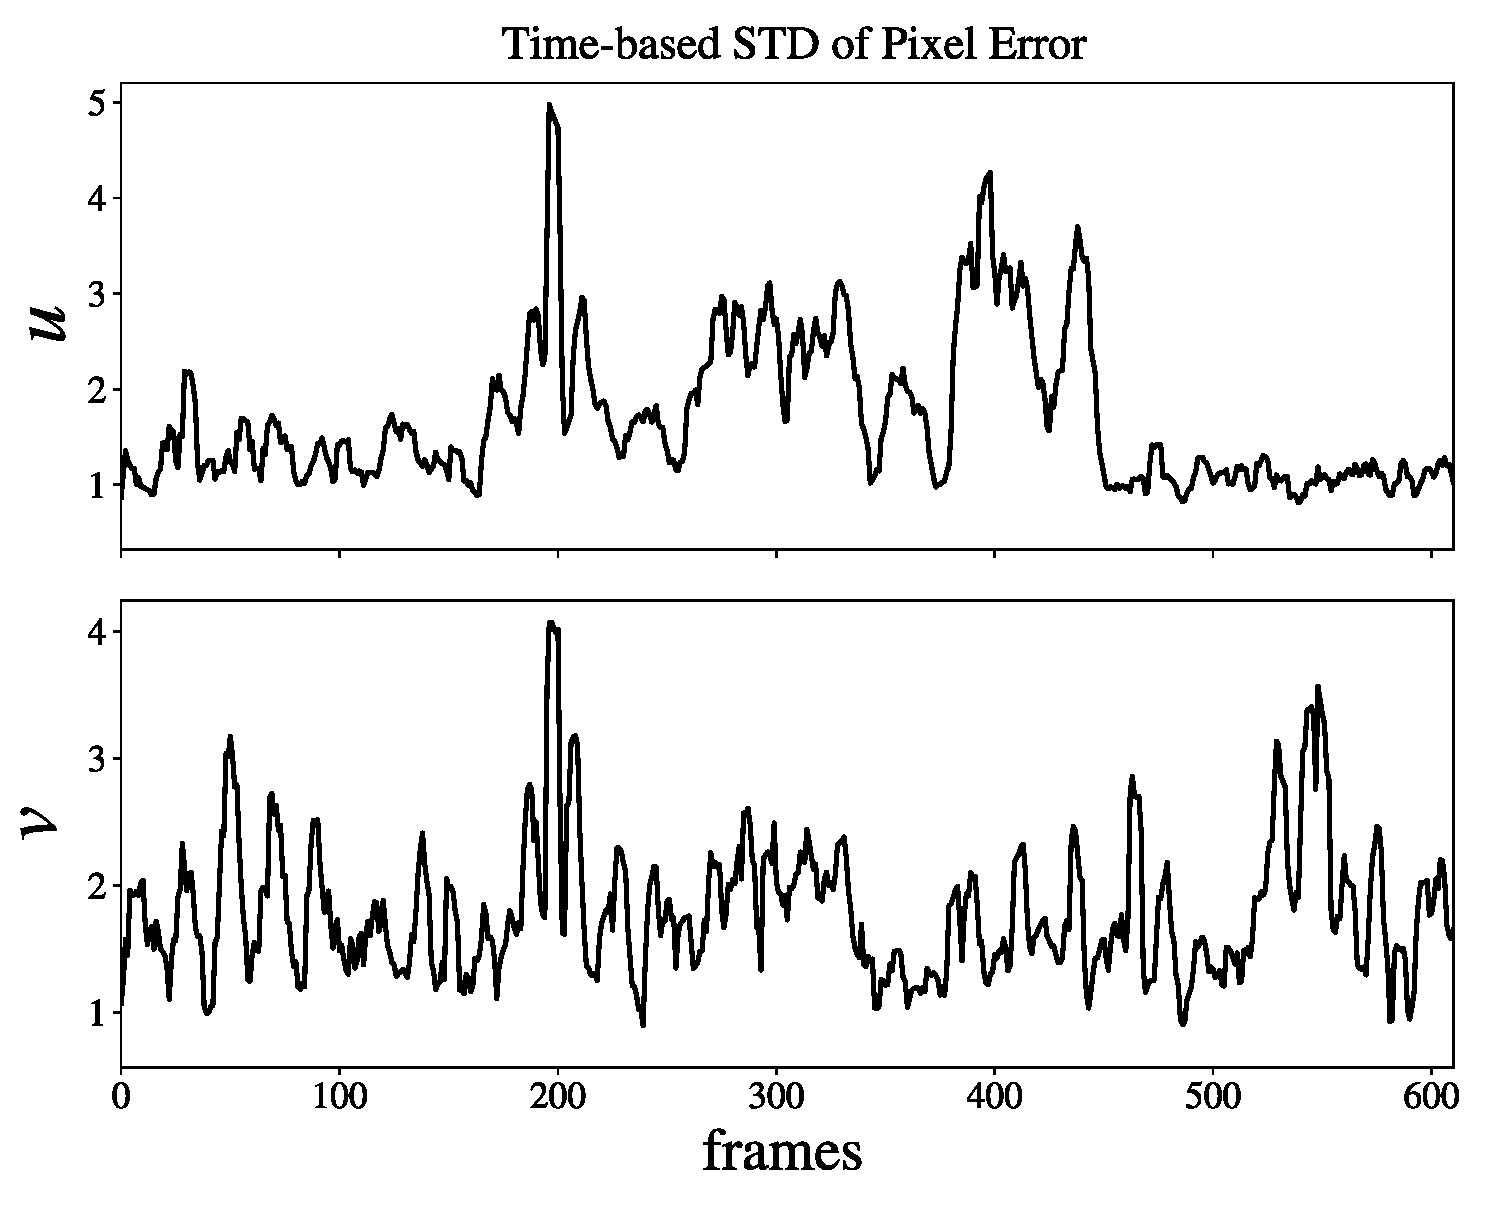
\includegraphics[width=\linewidth,natwidth=640,natheight=640]
  {fig/eva_graphs/tum_fr1_xyz_tbased_uv_err_std.pdf}
  \caption{asda}
\end{figure}\label{fig:time_based_std_pix_err}

The goal is to run this test over many datasets so that we can find the largest 
standard deviation. The result of these test are represented with 
the boxplots in figure \ref{fig:boxplot_time_based_std_all_datasets}.

% Boxplot of Time-based std with 5 frame sliding window for all datasets

\begin{figure}[H]
\begin{tabular}{ccc}
\centering
\subcaptionbox{fr1 xyz}{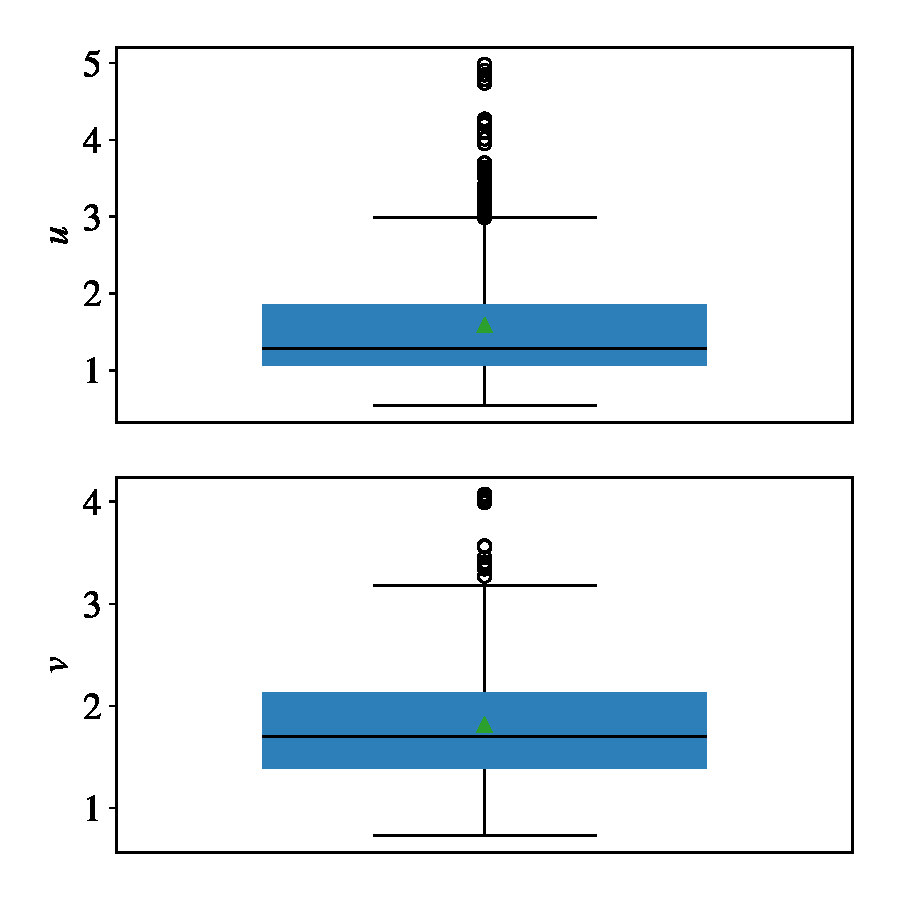
\includegraphics[width = 0.3\linewidth]{fig/eva_graphs/boxplot_tbased_uv_err_std_fr1_xyz.pdf}} &
\subcaptionbox{fr1 rpy}{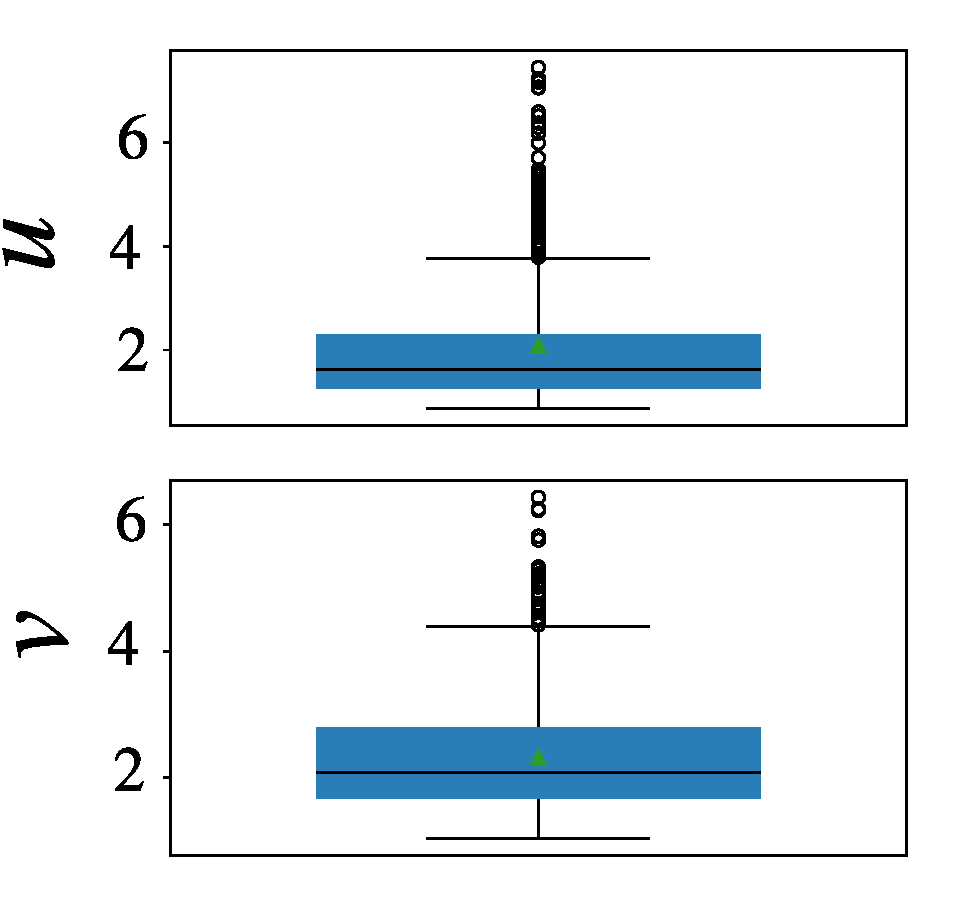
\includegraphics[width = 0.3\linewidth]{fig/eva_graphs/boxplot_tbased_uv_err_std_fr1_rpy.pdf}} &
\subcaptionbox{fr1 room}{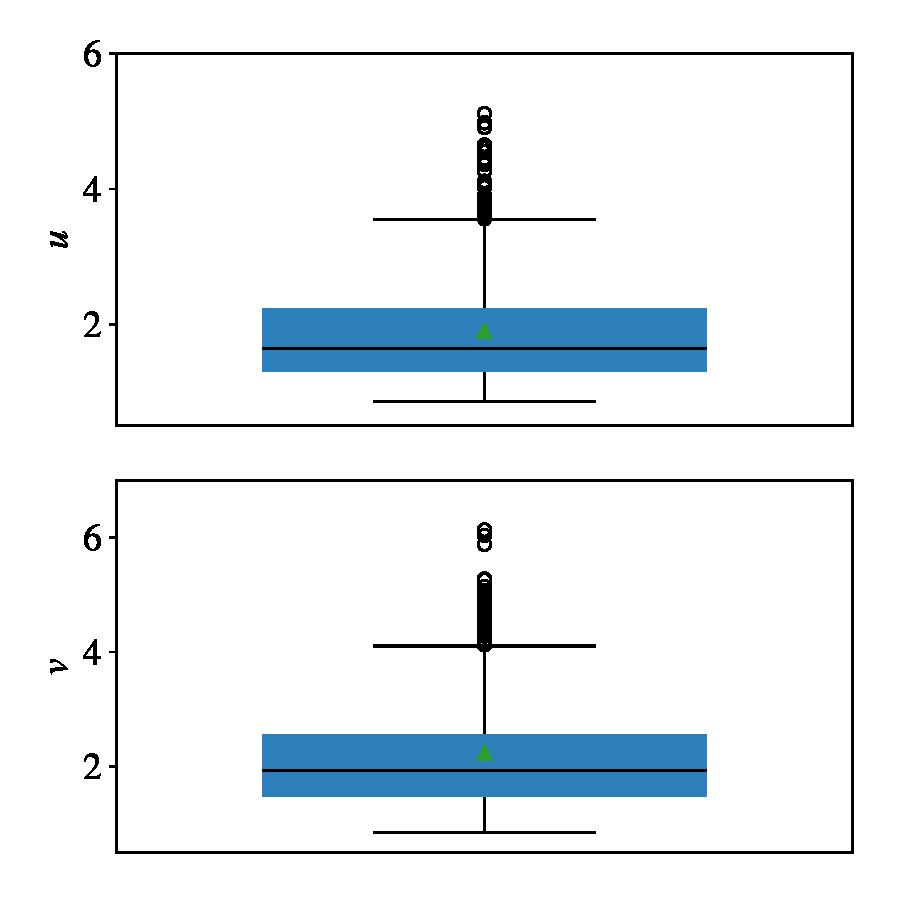
\includegraphics[width = 0.3\linewidth]{fig/eva_graphs/boxplot_tbased_uv_err_std_fr1_room.pdf}} \\
\subcaptionbox{fr1 360}{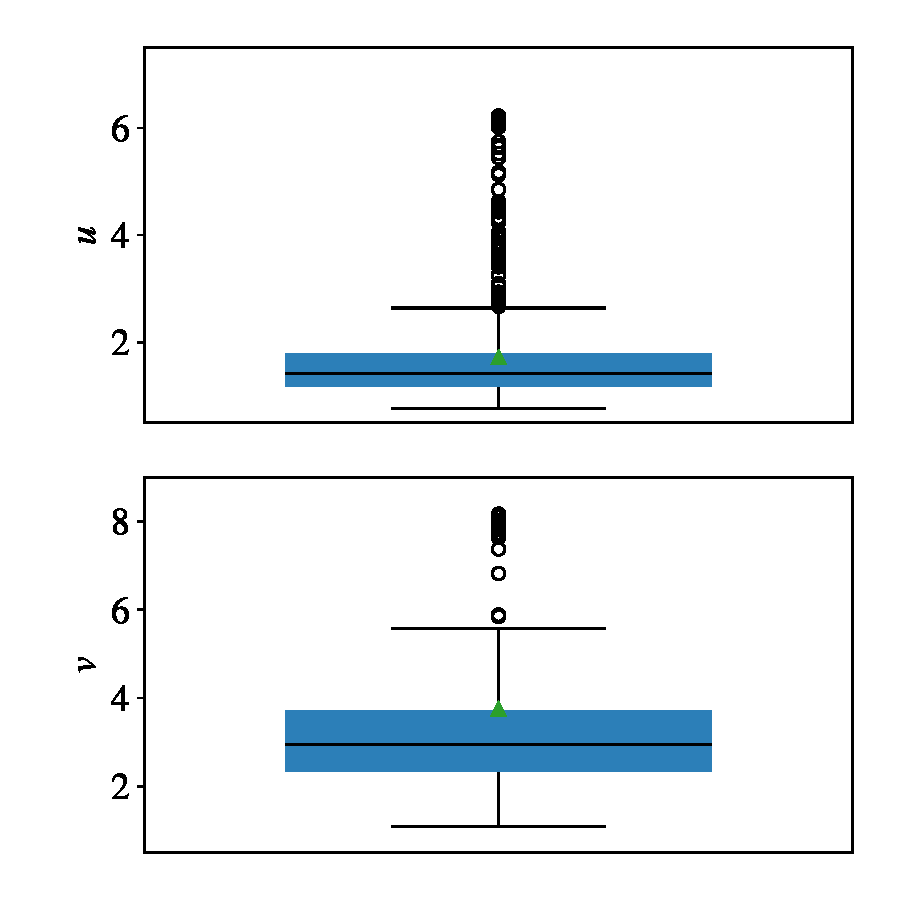
\includegraphics[width = 0.3\linewidth]{fig/eva_graphs/boxplot_tbased_uv_err_std_fr1_360.pdf}} &
\subcaptionbox{fr1 desk}{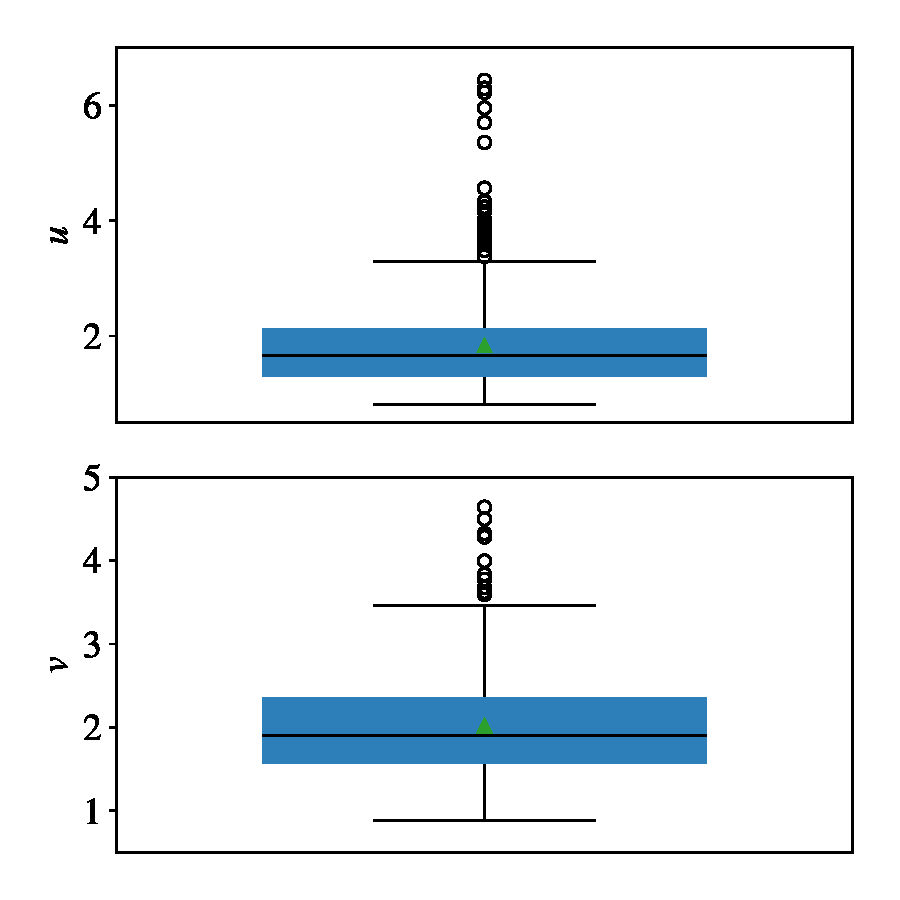
\includegraphics[width = 0.3\linewidth]{fig/eva_graphs/boxplot_tbased_uv_err_std_fr1_desk.pdf}} &
\subcaptionbox{fr1 desk2}{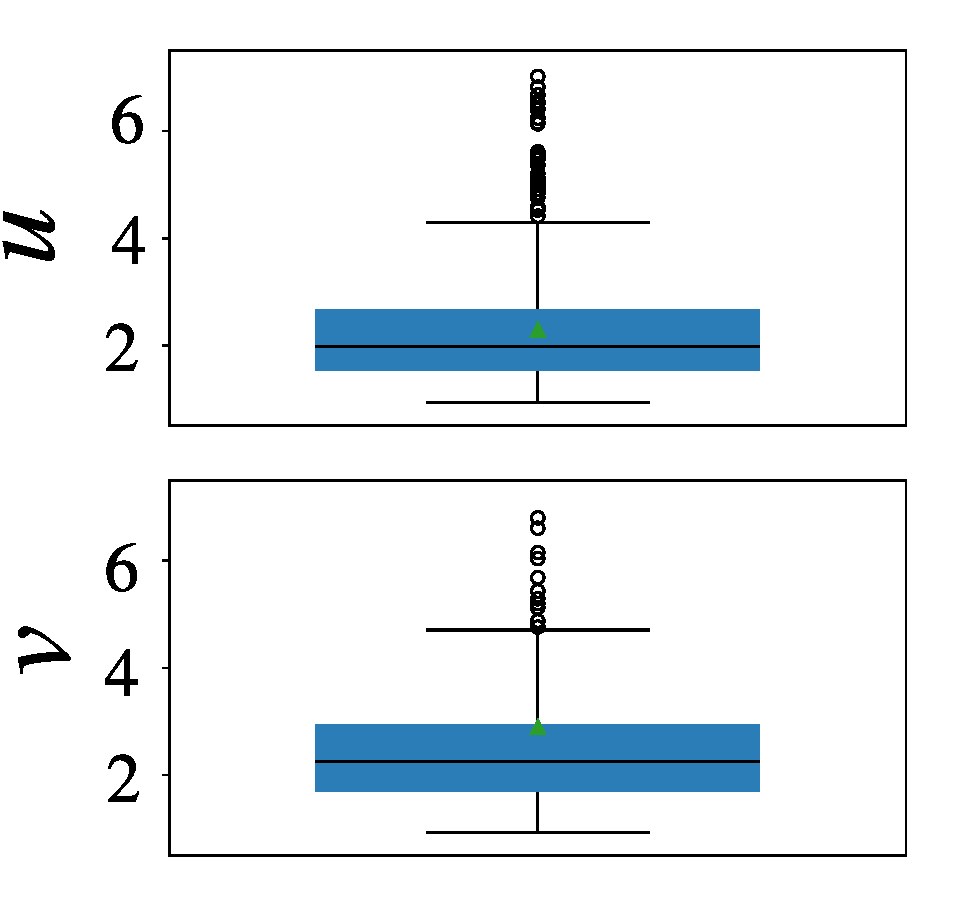
\includegraphics[width = 0.3\linewidth]{fig/eva_graphs/boxplot_tbased_uv_err_std_fr1_desk2.pdf}}
\end{tabular}
\caption{Remove Y axes title and Y axes thick from graphs!!!}
\end{figure}\label{fig:boxplot_time_based_std_all_datasets}

To cover the worst case scenario, 
we take these values as largest value of standard deviations of the pixel noise 
when forming covariance matrix $\mathbf{Q_{uvz}}^{(i,k)}$.

% 2

%\subsection{Estimation of Relative Pose and its Covariance}
%
%% 2.1
%% - Decide which one to use for scaling: RANSAC Threshold or max std?
%% -> DONE! Decided on max std besides the outliers due to wrong ground truth!
%% - Show estimated covariances that is scaled with RANSAC Threshold or Max std?
%
%% Translation RPE frame-to-frame with 3 sigma with fr1_xyz
%\begin{figure}[H]
%  \centering
%  \includegraphics[width=\linewidth,natwidth=640,natheight=640]
%  {fig/eva_graphs/tum_fr1_xyz_trans_rpe_3sigma.pdf}
%  \caption{asda}
%	\label{fig:2d_local_coords_in_world_coords}
%\end{figure}
%
%
%% Rotation RPE frame-to-frame with 3 sigma with fr1_xyz
%\begin{figure}[H]
%  \centering
%  \includegraphics[width=\linewidth,natwidth=640,natheight=640]
%  {fig/eva_graphs/tum_fr1_xyz_rot_rpe_3sigma.pdf}
%  \caption{asda}
%	\label{fig:2d_local_coords_in_world_coords}
%\end{figure}
%

% 1
\subsection{Evaluation of Estimated Covariance}\label{sc_cov_eval}

Similar to simulation data, we calculate NEES for covariance of the estimated 
poses after running the VO algorithm 6 different datasets in TUM. 
Note that we set standard deviation of pixel uncertainty according to 
the largest value $\sigma_u=7$ and $\sigma_v=8$ 
determined in the experimental analysis done in previous section.
After each optimization, we scale resulting covariance $\mathbf{Q_{t,q}}^{(k,k+1)}$
with the $\phi=4^2$ to compensate the errors due to the linearization.
Under these parameterizations, we run the algorithm and calculate 
histogram of NEES and ANEES for the selected datasets. 
The resulting histograms are illustrated in \ref{fig:hist_nees_all_datasets} and 
their ANEES are given in table \ref{tb:anees_all_datasets}.


%% NEES and ANEES with fr1_xyz
%\begin{figure}[H]
%  \centering
%  \includegraphics[width=\linewidth,natwidth=640,natheight=640]
%  {fig/eva_graphs/tum_fr1_xyz_nees.pdf}
%  \caption{asda}
%	\label{fig:2d_local_coords_in_world_coords}
%\end{figure}

% Without average by 3 (degree of freedom)
%fr1 xyz
%Translation Average NEES: 24.102167961194326
%Rotation Average NEES: 52.094722966630314
%fr1 360 
%Translation Average NEES: 23.056611560549662
%Rotation Average NEES: 75.33737874564399
%fr1 rpy 
%Translation Average NEES: 21.70951280913415
%Rotation Average NEES: 64.33137984284465
%fr1 desk
%Translation Average NEES: 60.40113749011506
%Rotation Average NEES: 105.36408125491856
%fr1 desk2
%Translation Average NEES: 56.536957402794926
%Rotation Average NEES: 110.9844039603292
%fr1 room 
%Translation Average NEES: 19.81107198582873
%Rotation Average NEES: 55.49945876186048

% Histogram of NEES with all datasets!
% BUG: Caption does not located under figures!
\begin{figure}[H]
\begin{tabular}{ccc}
\centering
\subcaptionbox{fr1 xyz}{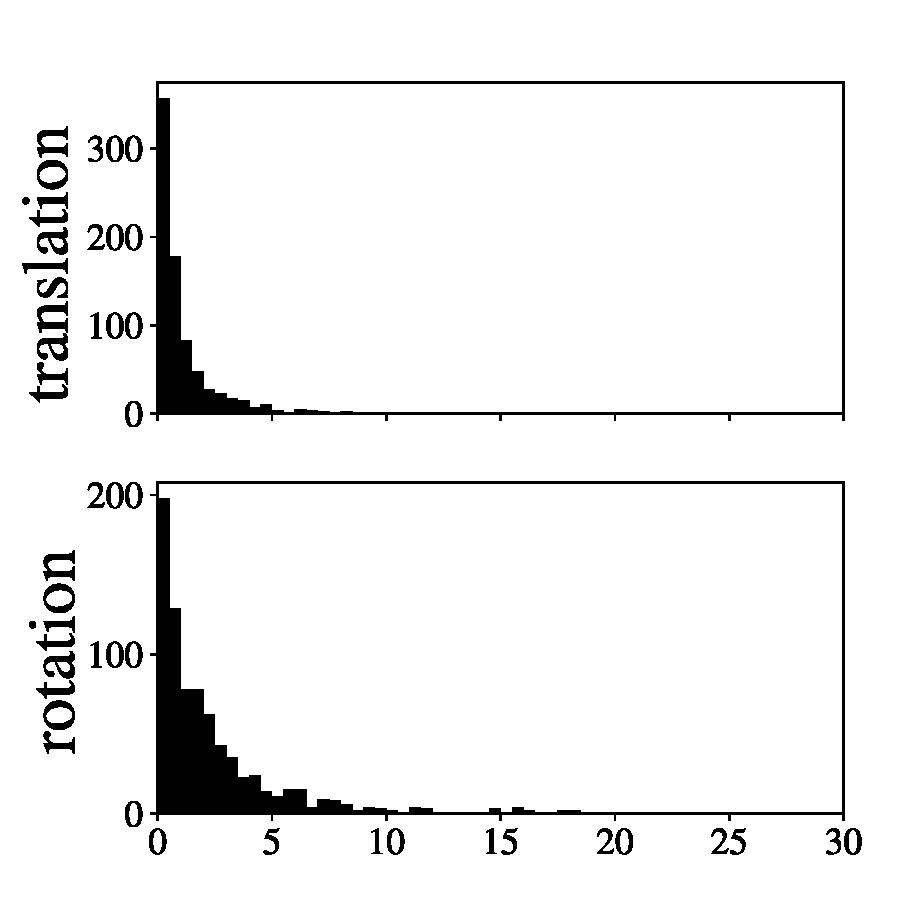
\includegraphics[width = 0.3\linewidth]{fig/eva_graphs/tum_fr1_xyz_hist_nees.pdf}} &
\subcaptionbox{fr1 rpy}{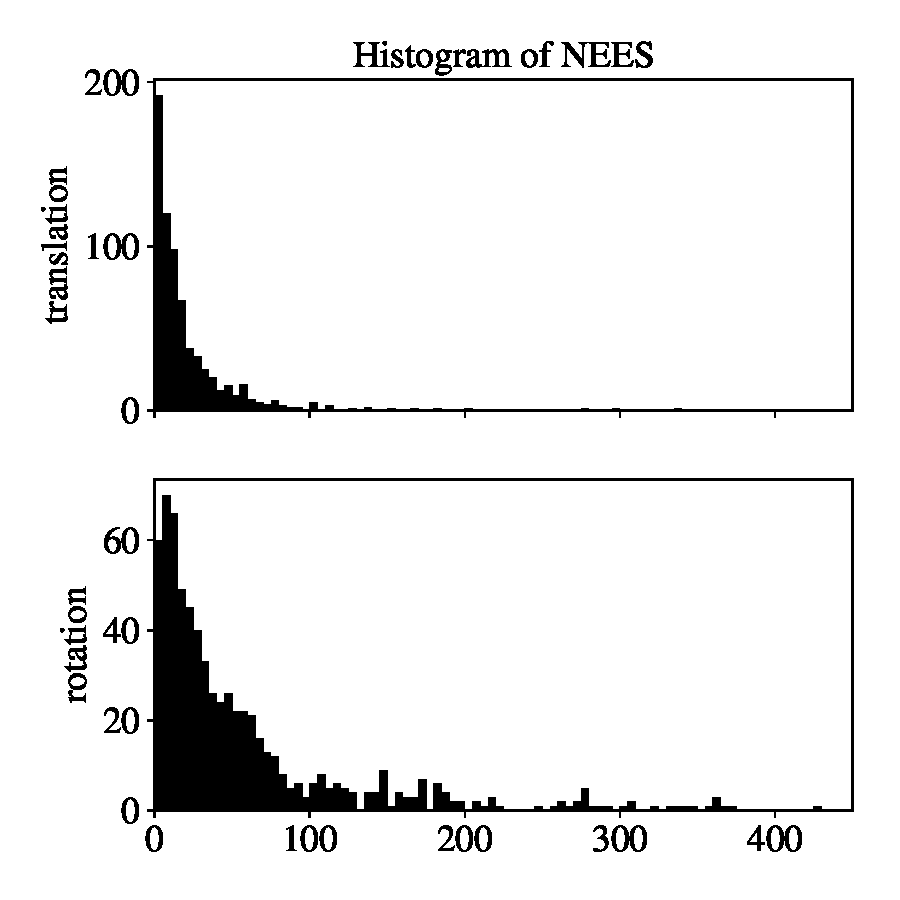
\includegraphics[width = 0.3\linewidth]{fig/eva_graphs/tum_fr1_rpy_hist_nees.pdf}} &
\subcaptionbox{fr1 room}{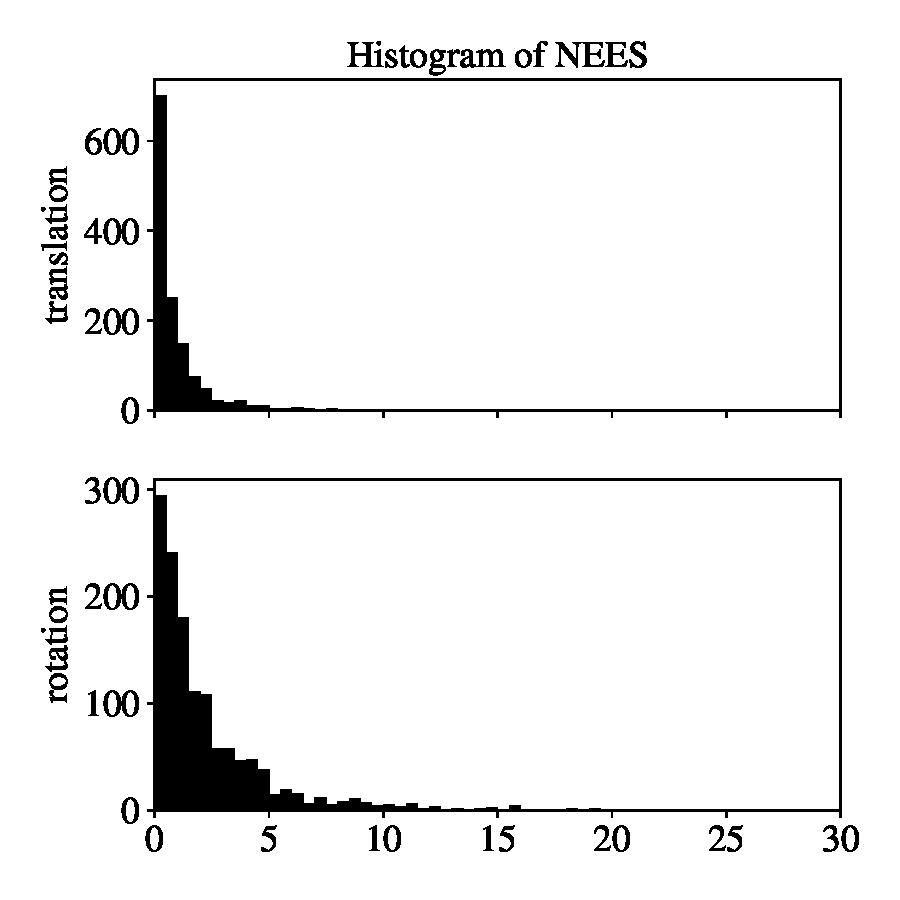
\includegraphics[width = 0.3\linewidth]{fig/eva_graphs/tum_fr1_room_hist_nees.pdf}} \\
\subcaptionbox{fr1 360}{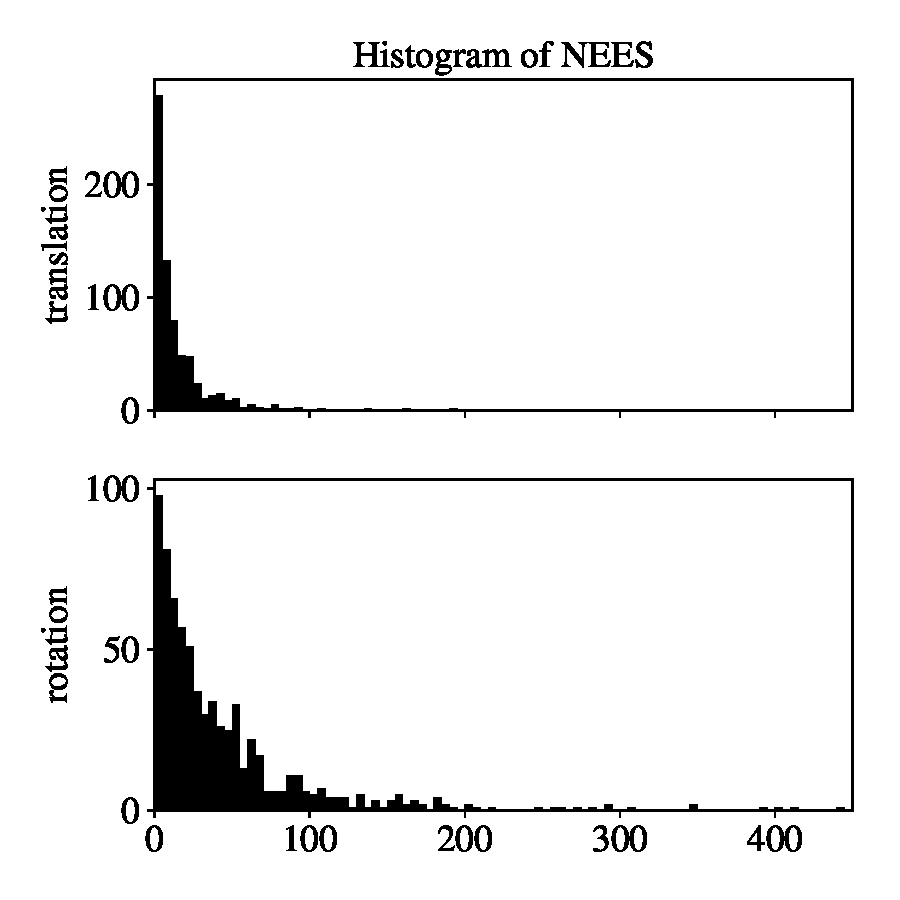
\includegraphics[width = 0.3\linewidth]{fig/eva_graphs/tum_fr1_360_hist_nees.pdf}} &
\subcaptionbox{fr1 desk}{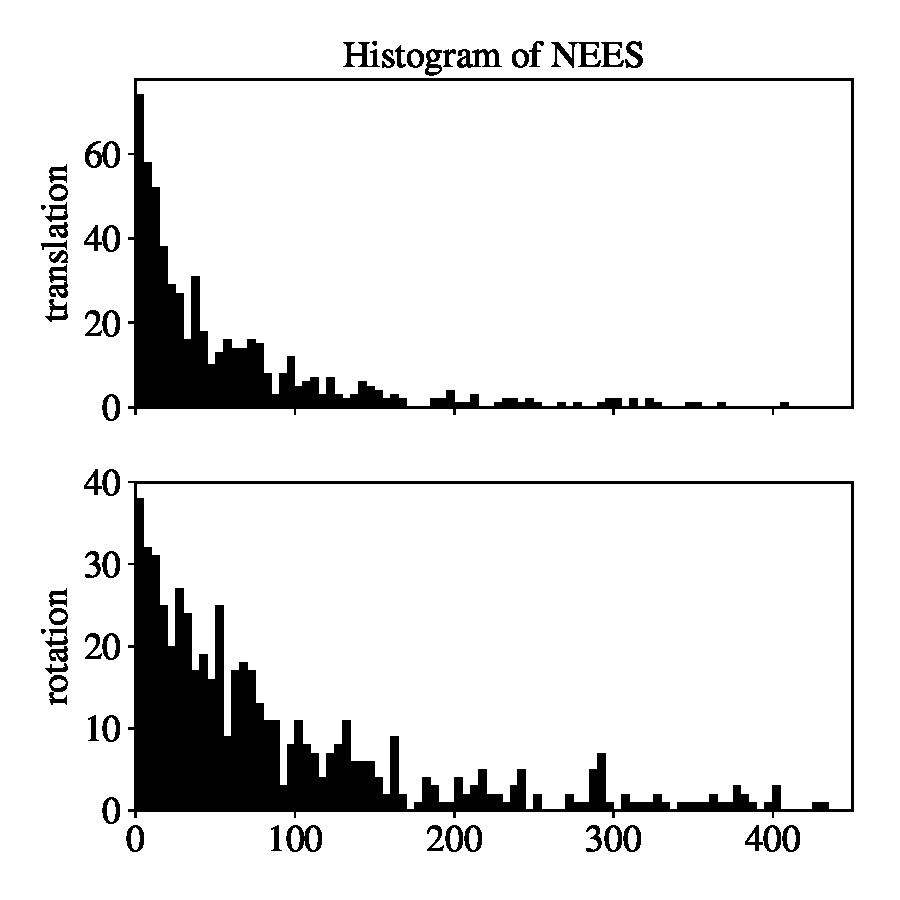
\includegraphics[width = 0.3\linewidth]{fig/eva_graphs/tum_fr1_desk_hist_nees.pdf}} &
\subcaptionbox{fr1 desk2}{\includegraphics[width = 0.3\linewidth]{fig/eva_graphs/tum_fr1_desk2_hist_nees.pdf}}
\end{tabular}
\caption{4 x 4}
\end{figure}\label{fig:hist_nees_all_datasets}

We observe that covariance of the translation estimations are conversative, 
which is acceptable in VO systems. However, covariance of the rotation estimation 
result in being overconfident for 3 datasets; i.e., 'fr1 360', 'fr1 desk' and 'fr1 room'.
Thus, we can say the estimator is \textit{inconsistent} for the rotation, 
as opposed to the translation providing consistent covariance estimations.

\begin{center}
  \begin{tabular}{l|cc|cc}
    \hline
  & Translation ANEES & Status & Rotation ANEES & Status \\
  \hline
  fr1 xyz   & 1.55 & conservative & 2.48 & conservative \\
  \hline
  fr1 rpy   & 1.08 & conservative & 3.10 & conservative \\
  \hline
  fr1 360   & 1.21 & conservative & 3.69 & overconfident \\
  \hline
  fr1 desk  & 2.88 & conservative & 4.99 & overconfident \\
  \hline
  fr1 desk2 & 2.72 & conservative & 5.30 & overconfident \\
  \hline
  fr1 room  & 0.96 & conservative & 2.65 & conservative \\
  \hline
  \end{tabular}
\end{center}\label{tb:anees_all_datasets}


% 5
\section{Comparison to FOVIS}

%subsection{Trajectory Estimation}
As for the accuracy of the estimated poses, we compare the proposed algorithm 
with FOVIS, which is a defacto VO application since it produces very accurate 
pose estimation with fast computations.
To provide an illustration as to building trajectory from relative pose estimations, 
we draw estimations results of 'fr2 desk' which is suitable to present drift effects 
and it is given in \ref{fig:comp_fr2_desk} along with the boxplot representation
of RPEs. 

% Traj XYZ with fr2_desk Boxplot with fr2_desk
\begin{figure}[H]
\begin{tabular}{ccc}
\centering
\subcaptionbox{asd}{\includegraphics[width = 0.5\linewidth]{fig/eva_graphs/fovis_comp_3d_tum_fr2_desk.pdf}} &
\subcaptionbox{asd}{\includegraphics[width = 0.45\linewidth]{fig/eva_graphs/fovis_comp_boxplot_tum_fr2_desk.pdf}}
\end{tabular}
\caption{Remove Y axes title and Y axes thick from graphs!!!}
\end{figure}\label{fig:comp_fr2_desk}

We run both algorithm for the 7 datasets and the resulting RMSEs of RPEs 
are given in table \ref{tb:comp_all_dataset}. Note that we take $\Delta=30$ 
frames while calculating RPEs.

\begin{figure}[H]
\begin{tabular}{ccc}
\centering
\subcaptionbox{fr1 xyz}{\includegraphics[width = 0.3\linewidth]{fig/eva_graphs/fovis_comp_boxplot_tum_fr1_xyz.pdf}} &
\subcaptionbox{fr1 rpy}{\includegraphics[width = 0.3\linewidth]{fig/eva_graphs/fovis_comp_boxplot_tum_fr1_rpy.pdf}} &
\subcaptionbox{fr1 room}{\includegraphics[width = 0.3\linewidth]{fig/eva_graphs/fovis_comp_boxplot_tum_fr1_room.pdf}} \\
\subcaptionbox{fr1 360}{\includegraphics[width = 0.3\linewidth]{fig/eva_graphs/fovis_comp_boxplot_tum_fr1_360.pdf}} &
\subcaptionbox{fr1 desk}{\includegraphics[width = 0.3\linewidth]{fig/eva_graphs/fovis_comp_boxplot_tum_fr1_desk.pdf}} &
\subcaptionbox{fr1 desk2}{\includegraphics[width = 0.3\linewidth]{fig/eva_graphs/fovis_comp_boxplot_tum_fr1_desk2.pdf}}
\end{tabular}
\caption{4 x 4}
\end{figure}


\begin{center}
  \begin{tabular}{lcc}
    \hline
    & FOVIS & COVO\\
     & RMSE & RMSE\\
    \hline
    fr1 xyz   & 0.0240  & 0.0512\\ 
    \hline
    fr1 rpy   & 0.0533  & 0.0368\\
    \hline
    fr1 360   & 0.0867  & 0.1239\\ 
    \hline
    fr1 desk  & 0.0406  & 0.0665\\
    \hline
    fr1 desk2 & 0.0533  & 0.0941\\
    \hline
    fr1 room  & 0.0587  & 0.0791\\
    \hline
    fr2 desk2 & 0.0156  & 0.0428 \\
    \hline
  \end{tabular}\label{tb:comp_all_dataset}
\end{center}

We can say that FOVIS is more accurate than the proposed algorithm and 
name number of reasons. FOVIS utilizes the keyframe scheme and different 
outlier rejection algorithm than RANSAC and 
provides a better initial guess to its optimizer after several refinement processes 
throughout the pipeline.





\chapter{Conclusion} \label{cp_conc}

% what&how I did in 2-3 sent

This thesis was undertaken to design
an error-aware RGB-D Visual Odometry system and evaluate its credibility. 
This achieved by identifying the errors occuring in both sensor 
and algorithm level and integrating them into the optimization 
problem.

% outline thesis
After an introduction chapter, the first step was to lay out 
the foundational elements of Visual Odometry.
% camera model
Then, the geometrical models of a RGB-D camera sensor was given 
in order to be acquainted with the working principles of such sensors 
in Chapter 2. 
The pinhole and triangulation models 
served as essential tools when modeling error characteristics of the sensors.
% typical vo pipeline
In Chapter 3, the typical pipeline of a feature based VO 
was studied. The pipeline comprised of 4 fundamental processes; that is, 
extracting features, matching features, rejecting outliers and 
pose estimation. To model uncertainy of the complete system, 
not only the systematic errors of the sensors, but also 
the errors introduced by the image processing processes are 
needed to be investigated.

% modeling uncertainties of RGB-D
After stating the motivation behind the thesis in Chapter 4, two main source of errors 
are discussed in Chapter 5; i.e., feature related errors caused by outliers and 
depth related errors caused by the IR sensor.  
All of these errors were combined in the conic ray model to 
represent the uncertainty of 3D feature points with covariances.
% optimization 
Afterwards, how these uncertainties were incorporated 
into the optimization process and 
the covariance of the estimated pose was propagated through 
feature uncertainty were described in detail.

% evaluation 
Chapter 6 started with presenting the simulation environment whose purpose 
is to validate the corectness of the algorithm.
% sim 
Experiments in simulation showed that linearization
of projection function led to inconsistency for the covariance 
of the estimated poses in the case of large noise. 
This issue was compensated with a heuristic method that 
scales resulting covariance accordingly.
% tum dataset
Next, TUM RGB-D dataset was used 
not only for testing 
consistency of the estimations with the real-world data, 
but also for identifying the effect of pseudo inliers 
on pixel uncertainty. 
% fovis comp
At the end of the chapther, 
accuracy of the proposed algorithm was compared with FOVIS.

% limitations
Finally, several limitations to this work need to be acknowledged. 
The simulation environment was built under the assumption that the 
pixel and depth uncertainties are gaussian and there are no outliers in 
feature matches. The fact that RANSAC is non-deterministic 
causes to remain outliers that are greater than RANSAC's acceptance 
threshold. Once remaining outliers are treated as pseudo inliers, 
pixel uncertainty grows, which then brings out issues in the linearizations.
It is also obvious that setting the pixel uncertainty 
by the largest standard deviation value
after running exhaustive tests 
to determine how pseudo inliers' error are distributed throughout all trajectories 
will not cover every corner cases. Thus, this problem requires more 
sophisticated approaches if more adaptive covariance estimation is desired.
Additionally, in contrast to our simulation environment, 
the analysis being done for estimator's consistency with NEES 
is usually performed in Monte Carlo simulation to introduce greater uncertainty 
to the system.

TODO: open questions and future work

\chapter{Bibliography} \label{cp_bib}

%deleting auto-generated reference title

% throws error
%\renewcommand\refname{\vskip -1cm} 

%\nocite{*}

%\bibliographystyle{alpha}
%\bibliography{/home/bolatu/Documents/mendeley_bib/Master_Thesis_Bib}

\printbibliography


% ***************************CP7-EVALUATION***************************
\chapter{Appendices} \label{cp_appendices}

\section{Rigid-Body Transformations} \label{sc_rigid_body_transformations}

\textit{Rigid-body} refers to objects made of solid materials so deformation is 
neglected. Thus, we idealize it by assuming that any given two points of 
rigid-body remains constant in time regardless of external forces 
applied on it. In $\R^3$ space, a rigid-body has 6 degree of freedom; i.e, 
3 for the position $(x, y, z)$ and 3 for the orientation $(\alpha, \beta, \gamma)$.
For a rigid-body, the motion is composed of a rotation around an axis and 
a translation along an axis. 

Let
$p_0=[\mathbf{t}, \mathbf{q}]^T=[t_x, t_y, t_z, q_x, q_y, q_z, q_w]^T$
be the initial pose of the frame that is fixed to the rigid-body 
where $\mathbf{t}$ represents the position and $\mathbf{q}$ rotation.

\subsubsection{Translation}

One can translate the rigid-body to another position with a simple vector 
addition operation:

\begin{equation}
\begin{aligned}
  \mathbf{t}_1 &= \mathbf{t}_0 + \mathbf{t}_{01}\\
  \begin{bmatrix} t_x^1 \\ t_y^1 \\ t_z^1 \end{bmatrix} & = 
  \begin{bmatrix} t_x^0 \\ t_y^0 \\ t_z^0 \end{bmatrix} + 
  \begin{bmatrix} t_x^{01} \\ t_y^{01} \\ t_z^{01} \end{bmatrix}
\end{aligned}
\end{equation}

\begin{figure}[H]
\begin{tabular}{ccc}
\centering
\subcaptionbox{p0}{\includegraphics[width = 0.45\linewidth]{fig/eva_graphs/append_p0.pdf}} &
\subcaptionbox{p1}{\includegraphics[width = 0.45\linewidth]{fig/eva_graphs/append_p1_trans.pdf}}
\end{tabular}
\caption{}
\end{figure}\label{fig:}


\subsubsection{Rotation with Quaternions}

One can rotate the rigid-body to another orientation with the 
quaternion product:

\begin{equation}
\begin{aligned}
  \mathbf{q}_1 &= \mathbf{q}_{01} \otimes \mathbf{q}_0\\
  \mathbf{q}_1 &= [\mathbf{q}_{01}]_L \mathbf{q}_0\\
  \begin{bmatrix} 
    q_w^{01} q_w^0 - q_x^{01} q_x^0 - q_y^{01} q_y^0 - q_z^{01} q_z^0  \\ 
    q_w^{01} q_x^0 + q_x^{01} q_w^0 + q_y^{01} q_z^0 - q_z^{01} q_y^0  \\ 
    q_w^{01} q_y^0 - q_x^{01} q_z^0 + q_y^{01} q_w^0 + q_z^{01} q_x^0  \\ 
    q_w^{01} q_z^0 + q_x^{01} q_y^0 - q_y^{01} q_x^0 + q_z^{01} q_w^0  
  \end{bmatrix} & = 
  \begin{bmatrix} 
    q_w^{01} - q_x^{01} - q_y^{01} - q_z^{01}  \\ 
    q_w^{01} + q_x^{01} + q_y^{01} - q_z^{01}  \\ 
    q_w^{01} - q_x^{01} + q_y^{01} + q_z^{01}  \\ 
    q_w^{01} + q_x^{01} - q_y^{01} + q_z^{01}  
  \end{bmatrix}
  \begin{bmatrix} q_w^0 \\ q_x^0 \\ q_y^0 \\ q_z^0 \end{bmatrix}
\end{aligned}
\end{equation}

where $[\mathbf{q}_{01}]_L$ is the left quaternion product in matrix form.

\begin{figure}[H]
\begin{tabular}{ccc}
\centering
\subcaptionbox{p0}{\includegraphics[width = 0.45\linewidth]{fig/eva_graphs/append_p0.pdf}} &
\subcaptionbox{p1}{\includegraphics[width = 0.45\linewidth]{fig/eva_graphs/append_p2_rot.pdf}}
\end{tabular}
\caption{}
\end{figure}\label{fig:}


\subsubsection{Transformation}

The most useful motion is the roto-translation motion, also called transformation, 
which rotates the rigid-body and then tanslates it:

\begin{equation}
  \mathbf{t}_1 = \mathbf{q}_{01} \otimes \mathbf{t'}_0 \otimes \mathbf{q}^*_{01} + \mathbf{t'}_{01}
\end{equation}

\begin{equation}
  \mathbf{q}_1 = \mathbf{q}_{01} \otimes \mathbf{q}_0\\
\end{equation}

where $\mathbf{t'}=[0, t_x, t_y, t_z]^T$ is the quaternion version of 
a vector $\mathbf{t}$ with zero scalar part.

\begin{figure}[H]
\begin{tabular}{ccc}
\centering
\subcaptionbox{p0}{\includegraphics[width = 0.45\linewidth]{fig/eva_graphs/append_p0.pdf}} &
\subcaptionbox{p1}{\includegraphics[width = 0.45\linewidth]{fig/eva_graphs/append_p3_trans_rot.pdf}}
\end{tabular}
\caption{}
\end{figure}\label{fig:}


\section{Least Squares}\label{sc_least_squares}

Throughout this thesis, least squares method empowered many different components 
of out VO system, 
such as camera calibration, RANSAC and most importantly motion estimation, 
Therefore, we will discuss underlying principles of least squares method in this section.

Ultimately, error minimization is an 
operation which wish to get the maximum likelihood of the function. To do so,
we search the most
likely state configuration as close as possible to its exact and ideal solution. 
In the case of any optimization problems,
the goal is to find interesting points, such as local/global
maximum or local/global minimum, on the \textit{objective}
\textit{function}. However, the exact model $F(\mathbf{x})$ of a system 
mostly unknown due to the high-degree for non-linearty or lack of knowledge.
Additionally, one needs to model the noise characteristics of measurements 
in real-world. This noise modeling also requires an approximation. 
Thus, one can only (hopefully) find a good enough solution by iteratively searching.
One way to solve effectively such problems is to generate a quadratic model of 
the objective function around initial guess $\mathbf{x}^0$ and iterate
through the function using the \textit{Newton's methods} or its variations.
For example,
an optimal solution (or an interest point)
figure \ref{fig:lsq_multivariable_function_example} is at the local
minimum of the function that is highlighted as a red point cloud.

\begin{figure}[H]
	\centering
	\includegraphics[width=\linewidth,natwidth=640,natheight=640]
	{fig/lsq_multivariable_function_example.jpg}
	\caption{Local Minimum at a Quadratic Function}
	\label{fig:lsq_multivariable_function_example}
\end{figure}


%In optimization literature,
%there are many versions of Newton's method 
%and they all try to find the
%local maximum/minimum in the most efficient and accurate way.

%However, in the end, they all solve the problem
%with the \textit{gradient descent} manner.
%the approximated Hessian function, is one of them and we will be using
%it in our slam algorithm.

To elaborate the problem, we provide a regression example 
which can be infact solved with linear least squares techniques but it can serve 
as a simple toy example throughout our explainations.

Suppose that we have a model function $g(\mathbf{x};a)$. However,
we don't know what the $\mathbf{x}=(x_1,x_2)$ coefficients (so-called
\textit{optimization} \textit{parameters}) are and we can only
plug $a$, which is the \textit{independent} variable, into the
\textit{model} $S$ to see
how the output of the model changes given the independent variable. 

\begin{figure}[H]
	\includegraphics[width=0.8\linewidth,natwidth=640,natheight=640]
	{fig/lsq_model.jpg}
	\centering
	\caption{Least Square Model}
	\label{fig:lsq_model}
\end{figure}



\begin{gather}
\xi = a \text{ (independent variable)} \in \R \\
\eta = S \text{ (dependent variable)} \in \R
\label{eq:lsq_model_variables}
\end{gather}

\begin{equation}
  S = g(\mathbf{x};a) := x_1 + x_2a \quad 
\text{where} \quad 
\mathbf{x} \in \R^2
\label{eq}
\end{equation}


To see this effect, 
we draw a graph that is shown in
figure \ref{fig:lsq_curve_fit_measurements}.

\begin{figure}[H]
	\centering
	\includegraphics[width=\linewidth,natwidth=640,natheight=640]
{fig/lsq_curve_fit_measurements_v2.jpg}
	\caption{Least Squares Measurements}
	\label{fig:lsq_curve_fit_measurements}
\end{figure}


Our goal is now to find a function, which will fit this
dataset. This is a typical least squares curve fitting problem.
In this problem, we construct a \textit{residuals function} $r_i(\mathbf{x})$ by providing
error values between model estimation $g(x;a_i)$ and dependent
variable $S_i$. In this case, the dependent variable 
represent the real world
measurements and the residuals function represents the error between the estimated value and measurement value. 

\begin{equation}
  r_i(\mathbf{x}) := g(\mathbf{x};a_i) - S_i \qquad \text{ for }  i = 1,\dots,m.
\label{eq:}
\end{equation}

The residuals function is usually squared to magnify larger error effect:

\begin{equation}
\begin{aligned}
  F(\mathbf{x}) & = \sum_{i=1}^{m} \vert r_i(\mathbf{x}) \vert^2 = 
  \sum_{i=1}^{m} \vert g(\mathbf{x};a_i) - S_i \vert^2 =
  \sum_{i=1}^{m} (g(\mathbf{x};a_i) - S_i)^2 \\
& = \begin{Vmatrix}
  \begin{pmatrix} g(\mathbf{x};a_1) - S_1 \\ \vdots \\ g(\mathbf{x};a_m) - S_m \end{pmatrix} 
\end{Vmatrix}_2^2
\label{eq}
\end{aligned}
\end{equation}

Now, one can use the sum of squared error function to calculate the most likely
configuration that can minimize the errors. 

\begin{equation}
  \mathbf{X}^* = \argmin_x F(\mathbf{x}) = 
  \sum_{i=1}^{m} (g(\mathbf{x};a_i) - S_i)^2, 
  \quad \mathbf{x} \in \R^2
\label{eq}
\end{equation}

At this point, the objective function is ready to be handed over to 
to any gradient decent based least squares solver. The method will try to find the
\textit{optimal} solution $\mathbf{X}^*$ by minimizing the objective function.

\begin{equation}
  \text{Minimize} \quad \sum_{i=1}^{m} (g(\mathbf{x};a_i) - S_i)^2, 
\quad \mathbf{x} \in \R^2
\label{eq}
\end{equation}

To help our understanding, the objective function is drawn in
figure \ref{fig:lsq_sum_of_squared_error_function}.
As we can see, the based on the given $\mathbf{x}$ values, 
the objective
function $F(\mathbf{x})$ behave as follows:

\begin{figure}[H]
	\centering
	\includegraphics[width=\linewidth,natwidth=640,natheight=640]
	{fig/lsq_sum_of_squared_error_function_v2.jpg}
	\caption{Local Minimum at Sum of Squared Error Function}
	\label{fig:lsq_sum_of_squared_error_function}
\end{figure}

The initial guess for the optimization parameters at $x=(4,4)$, which
is highlighted as a blue color point cloud and 
the local minimum point, which is the interest point of ours, 
is highlighted with the red cloud. What the gradient descent method essentially 
does is to travel from the initial guess point to the nearest local minimum 
on the objective function. As we can see
that the descent is successfully performed and the optimization
operation results at $\mathbf{x}=(1.9,2.1)$. 


If we now place the optimization variables into our model function, we
get the $g(\mathbf{x};a)=1.9+2.1a$ and a fitted line based on the given
dataset in
figure \ref{fig:lsq_curve_fit_operation}.

\begin{figure}[H]
	\centering
	\includegraphics[width=\linewidth,natwidth=640,natheight=640]
	{fig/lsq_curve_fit_operation_v2.jpg}
	\caption{Least Squares Curve Fitting Operation}
	\label{fig:lsq_curve_fit_operation}
\end{figure}

Now that we have an intiution how least squares problems are solved 
by gradient descent methods, let's further discuss one of them.

\subsection{The Newton's Method}

In order to understand non-linear least square algorithms, 
we first need to look at how the Newton's method works. 
It provides a guideline for finding roots of a function by 
taking differentiations of the function. The interesting phenomena is that the roots of 
function corresponds to the interest points of the function such as maximum, mimimum or 
saddle points. In least squares problem, we are only interested in minimum 
points since we want to minimize the error. Keeping this in mind, let's 
consider a non-linear objective function 
$F(\mathbf{x}) = \frac{1}{2}\mathbf{f(x)^Tf(x)} = \frac{1}{2}\sum_i f_i(\mathbf{x})^2$ 
where 
it has $\mathbf{x} = [x_1, \dots, x_n] \in R^n$ multiple unknown variables.
We also assume that the function $F(\mathbf{x})$ is differentiable with 
respect to each $x_i$ unknown variable and its 
first-order derivatives has the following form:

\begin{equation}
  \nabla F(\mathbf{x}) = \mathbf{J}_F = \mathbf{J_f^Tf}
\end{equation}

where $\mathbf{J}_F$ is the \textit{Jacobian} matrix that has a special matrix:

\begin{equation}
  \mathbf{J}_F = \begin{bmatrix} \frac{\partial}{\partial x_j }f_i(\mathbf{x}) \end{bmatrix}_{ij} 
  = 
  \begin{bmatrix} 
    \frac{\partial}{\partial x_1}f_1(\mathbf{x}) & \frac{\partial}{\partial x_2}f_1(\mathbf{x}) & \dots & \frac{\partial}{\partial x_n}f_1(\mathbf{x}) \\
    \frac{\partial}{\partial x_1}f_2(\mathbf{x}) & \frac{\partial}{\partial x_2}f_2(\mathbf{x}) & \dots & \frac{\partial}{\partial x_n}f_2(\mathbf{x}) \\
    \vdots & \vdots & \vdots & \vdots \\
    \frac{\partial}{\partial x_1}f_m(\mathbf{x}) & \frac{\partial}{\partial x_2}f_m(\mathbf{x}) & \dots & \frac{\partial}{\partial x_n}f_m(\mathbf{x}) \\
  \end{bmatrix}
  \in \R^{ixj}
\end{equation}


%\begin{figure}[H]
%	\centering
%	\includegraphics[width=\linewidth,natwidth=640,natheight=640]
%	{fig/ref_imgs/taylor_1st_derivative.png}
%	\caption{First-order Derivative of Taylor Expansion}
%  \label{fig:taylor_1st_derivative}
%\end{figure}

And the second-order derivatives has another special matrix for called 
\textit{Hessian}

\begin{equation}
\nabla^2 F(x) = \mathbf{H}_F
  = 
  \begin{bmatrix} 
    \frac{\partial^2}{\partial x_1^2}f_1(\mathbf{x}) & \frac{\partial^2}{\partial x_1x_2}f_1(\mathbf{x}) & \dots & \frac{\partial^2}{\partial x_1x_n}f_1(\mathbf{x}) \\
    \frac{\partial^2}{\partial x_2x_1}f_2(\mathbf{x}) & \frac{\partial^2}{\partial x_2^2}f_2(\mathbf{x}) & \dots & \frac{\partial^2}{\partial x_2x_n}f_2(\mathbf{x}) \\
    \vdots & \vdots & \vdots & \vdots \\
    \frac{\partial^2}{\partial x_nx_1}f_m(\mathbf{x}) & \frac{\partial^2}{\partial x_nx_2}f_m(\mathbf{x}) & \dots & \frac{\partial^2}{\partial x_n^2}f_m(\mathbf{x}) \\
  \end{bmatrix}
  \in \R^{mxn}
\end{equation}

Having first- and second-order derivatives helps us to 
form a so-called \textit{Newton} step:

\begin{equation}
  \Delta \mathbf{x}^n = - 
\frac{\nabla F(\mathbf{x}^n)}{\nabla^2 F(\mathbf{x}^n)} = - \mathbf{H}_F^{-1}\mathbf{J}_F
\end{equation}\label{eq:delta_x_descent_direction}

If we calculate the Netwon step, we know that $F(\mathbf{x})$ will decrease 
in the direction of its negative derivative if the step is added:
Then, one can 
claim that if we iteratively travel through the function in the direction of its negative 
derivative, we would eventually reach to a nearest local minima with respect to the starting 
point. 
%This is the fundamental idea behind any kind of gradient descent algorithm.
%While descenting, one might want to control the length of the Newton step, 
%For doing so, a tuning factor, called
%\textit{step length} $\alpha$, is used to adjust the size of length:
%
%\begin{equation}
%  \Delta \mathbf{x} = 
%  - \alpha \frac{F'(\mathbf{x^n})}{F''(\mathbf{x^n})} = - \alpha \mathbf{H}_F^{-1}\mathbf{J}_F
%\end{equation}\label{eq:delta_x_step_length}

%% WRONG THE NEWTONS METHOD DOES NOT CREATE QUAD FUNCTIONS!
%The analitical intuition behind how we calculate the Newton step is 
%to build a $q$ quadratic model of the objective function around the $\mathbf{x}^n$ 
%using Taylor expansion:
%
%\begin{equation}
%  q^n(\Delta \mathbf{x}) = F(\mathbf{x}^n) + 
%  \nabla F(\mathbf{x}^n)^T \Delta \mathbf{x} + \frac{1}{2} \Delta \mathbf{x}^T \nabla^2 F(\mathbf{x}^n)\Delta \mathbf{x}
%\end{equation}
%
%After $n$ number of iteration of $\mathbf{x}^n$, the $q(\mathbf{x}^n)$ 
%quadratic function will hugs (or fits to) the original function $F(\mathbf{x}^n)$ 
%at the $\mathbf{x}^{k+n} (= \mathbf{x^*})$.
%
%\begin{figure}[H]
%	\centering
%	\includegraphics[width=\linewidth,natwidth=640,natheight=640]
%	{fig/ref_imgs/taylor_2nd_derivative.png}
%\caption{REMOVE APPROX B - Second-order Derivative of Taylor Expansion}
%  \label{fig:taylor_2nd_derivative}
%\end{figure}
%

We can briefly describe the algorithm if 
assuming that we have an educated initial guess $\mathbf{x}^0$ from which 
we start to search 
for a local minimum, we can describe the Newton algorithm as follows:

\begin{enumerate}
  \item take the first- and second-order derivatives of $F(\mathbf{x})$ 
    at the current $\mathbf{x}^n$
  \item iterate $\mathbf{x}^{n+1} := \mathbf{x}^n -\Delta \mathbf{x}^n $ until it converges
\end{enumerate}

As we see, the Newton's method is a simple but an effective algorithm if 
we can calculate the first- and second-order derivatives accurately.
However, it is either computationally expensive to calculate Hessian or 
is unknown beforehand. Therefore, there are several variations of Newton's 
method, one of which will be discussed in next section.
%However, the problem can get very complicated 
%if convergence speed and convergence success is considered. For this reason, 
%there are many version of the algoritm that aims to solve the problem 
%in the most efficient manner.

\subsection{Levenberg-Marquardt}
Levenberg-Marquardt (LM) is one of most well-known algoritm 
to solve least squares problem. It is the modified version of the Netwon's 
method. In this section, we describe the idea behind 
the LM algorithm. Assume that we have a $\mathbf{r}(\mathbf{x}^n)$ residuals function which we 
wish to model:

\begin{equation}
  \mathbf{r}(\mathbf{x}^n) = \begin{pmatrix} r_1(\mathbf{x}^n) \\ \vdots \\ r_m(\mathbf{x}^n) \end{pmatrix} \in \R^m
\end{equation}

To find a local maximum/minimum of the residuals function, we need to 
determine the first derivative and it 
$\mathbf{r}'(\mathbf{x}^n)$ appears again in Jacobian form:

\begin{equation}
  \mathbf{J} = \frac{\partial \mathbf{r}(\mathbf{x}^n)}{\partial \mathbf{x}^n } \bigg|_{\mathbf{x}^n}
  = 
  \begin{bmatrix} 
    \vertbar & & \vertbar \\
    \frac{\partial}{\partial x_1}\mathbf{r}(\mathbf{x}^n) & \dots & \frac{\partial}{\partial x_n}\mathbf{r}(\mathbf{x}^n) \\
    \vertbar & & \vertbar
  \end{bmatrix}
  = 
  \begin{bmatrix}
    \horzbar & \nabla r_1(\mathbf{x}^n)^T & \horzbar \\
     & \vdots & \\
     \horzbar & \nabla r_m(\mathbf{x}^n)^T & \horzbar 
  \end{bmatrix}
  \in \R^{mxn}
\end{equation}

Least squares problem has special forms which can be exploitted. 
Here, the residuals function function and its derivatives is given:
%(Keep in mind that multiplication with $\frac{1}{2}$ in front of objective function
%is for cosmetic reason since it does not effect local mimimum's position in the function)

\begin{equation}
  F(\mathbf{x}) = \frac{1}{2} ||\mathbf{r}(\mathbf{x}^n)||^2 = \frac{1}{2} \mathbf{r}(\mathbf{x}^n)^T \mathbf{r}(\mathbf{x}^n) \text{  (Objective function)}
\end{equation}\label{eq:residuals_objective}
\begin{equation}
\nabla F(\mathbf{x}^n) = \mathbf{J}(\mathbf{x}^n)^T \mathbf{r}(\mathbf{x}^n) = \sum_{i=1}^{m} r_i(\mathbf{x}^n) \nabla r_i(\mathbf{x}^n) \text{  (First-order derivative)}
\end{equation}\label{eq:residuals_objective_first_der}
\begin{equation}
  \nabla^2 F(\mathbf{x}^n) = \mathbf{J}(\mathbf{x}^n)^T\mathbf{J}(\mathbf{x}^n) + \sum_{i=1}^m r_i(\mathbf{x}^n) \nabla^2 r_i(\mathbf{x}^n) \text{ (Second-order derivative)}
\end{equation}\label{eq:residuals_objective_second_der}


Given \ref{eq:residuals_objective} and \ref{eq:residuals_objective_first_der}, we elaborate the quadratic model:

\begin{equation}
  F(\mathbf{x}^n + \Delta \mathbf{x}) \approx
  q^n(\Delta \mathbf{x}) = 
  \frac{1}{2}\mathbf{r}(\mathbf{x}^n)^T\mathbf{r}(\mathbf{x}^n) + 
  \mathbf{r}(\mathbf{x}^n)^TJ(\mathbf{x}^n)\Delta \mathbf{x} + 
\frac{1}{2}\Delta \mathbf{x}^T(\mathbf{J}^T\mathbf{J}+\mathbf{r}(\mathbf{x}^n)^T\mathbf{H})^n\Delta \mathbf{x}
\end{equation}


\begin{equation}
  q_{LM}^n(\Delta \mathbf{x}) = \frac{1}{2}\mathbf{r}(\mathbf{x}^n)^T\mathbf{r}(\mathbf{x}^n) + \mathbf{r}(\mathbf{x}^n)^TJ(\mathbf{x}^n)\Delta \mathbf{x} + \frac{1}{2}\Delta \mathbf{x}^T\mathbf{B_{LM}}^n\Delta \mathbf{x}
\end{equation}


\begin{equation}
  0 = 
  \nabla q^{n}(\Delta \mathbf{x}^*) = 
  \mathbf{r}(\mathbf{x}^n)^TJ(\mathbf{x}^n) + 
(\mathbf{J}^T\mathbf{J}+\mathbf{r}(\mathbf{x}^n)^T\mathbf{H})^n\Delta \mathbf{x}^*
\end{equation}


\begin{figure}[H]
	\centering
	\includegraphics[width=\linewidth,natwidth=640,natheight=640]
	{fig/ref_imgs/taylor_2nd_derivative.png}
	\caption{Second-order Derivative of Taylor Expansion}
  \label{fig:taylor_2nd_derivative}
\end{figure}


It is critical to note that LM does not use $\nabla^2F(\mathbf{x})$ 
the exact second-order derivative (\ref{eq:residuals_objective_second_der})
(also appears in the special form called \textit{Hessian}) in its quadratic model. 
This is because it is computationaly expensive. Instead, we use an approximated 
Hessian model by removing $\sum_{i=1}^mr_i(\mathbf{x})\nabla^2r_i(\mathbf{x})$ and replacing with 
term $\lambda^n \mathbf{I}$. Finally, the final approximated Hessian function would be:

\begin{equation}
  \mathbf{B_{LM}}^n = \mathbf{J}(\mathbf{x}^n)^T \mathbf{J}(\mathbf{x}^n) + \lambda^n \mathbf{I}
\end{equation}

where $\lambda^n>0$ is a positive number and $\mathbf{I}\in \R^{kxk}$ is the identity matrix.

\begin{figure}[H]
	\centering
	\includegraphics[width=\linewidth,natwidth=640,natheight=640]
	{fig/ref_imgs/taylor_approx_2nd_derivative.png}
	\caption{Approximated Second-order Derivative of Taylor Expansion}
  \label{fig:taylor_approx_2nd_derivative}
\end{figure}




Similar to \ref{eq:delta_x_descent_direction}, one can calculate the descent direction 
in the context of LM method as follows:

\begin{equation}
  \mathbf{B_{LM}}^n \Delta \mathbf{x}^n = - \nabla F(\mathbf{x}^n) \text{ or } \Delta \mathbf{x}^n = - (\mathbf{B_{LM}}^n)^{-1}\nabla F(\mathbf{x}^n)
\end{equation}\label{eq:lm_descent_direction}

If we can write above equation using the content of Hessian model more explicitly: 

\begin{equation}
  [\mathbf{J}(\mathbf{x}^n)^T\mathbf{J}(\mathbf{x}^n) + \lambda^n\mathbf{I}]\Delta \mathbf{x}^n = -\mathbf{J}(\mathbf{x}^n)^T\mathbf{r}(\mathbf{x}^n)
\end{equation}\label{eq:damping_full}

it gives a clearer picture why $\lambda^nI$ term is used. In other gradient-descent 
based algorithm performs line search to determine the step length of the current 
iteration. In LM, this is done by tuning $\lambda$ parameter, also known as 
\textit{damping parameter}. For example, suppose that we assign $\lambda$ 
a significantly small value. Then, \ref{eq:damping_full} becomes:

\begin{equation}
  \lambda^n\Delta \mathbf{x}^n \approx -\mathbf{J}(\mathbf{x}^n)^T\mathbf{r}(\mathbf{x}^n) \text{ or } 
  \Delta \mathbf{x}^n \approx -\frac{1}{\lambda^n}\mathbf{J}(\mathbf{x}^n)^T\mathbf{r}(\mathbf{x}^n)\text{ or } 
  \Delta \mathbf{x}^n \approx -\frac{1}{\lambda^n}\nabla F(\mathbf{x}^n)
\end{equation}

Whereas, if we assign $\lambda$ a significantly large value, then it becomes:

\begin{equation}
  \mathbf{J}(\mathbf{x}^n)^T\mathbf{J}(\mathbf{x}^n)\Delta \mathbf{x}^n = -\mathbf{J}(\mathbf{x}^n)^T\mathbf{r}(\mathbf{x}^n)
\end{equation}

which is a regular \textit{Newton step} (corresponds to $\alpha=1$ in \ref{eq:delta_x_step_length}).

On the other hand, another question arises about damping parameter about how to tune the parameter 
so that it will allow the algorithm to converge to a local minimum efficiently 
and accurately. This is done by the \textit{progress ratio} test:

\begin{equation}
  \rho^n = \frac{F(\mathbf{x}^n) - F(\mathbf{x}^n+\Delta \mathbf{x})}{q_{LM}^n(\mathbf{0})-q_{LM}^n(\Delta \mathbf{x})} =
  \frac{\text{actual decrease in objective } F(\mathbf{x})}
  {\text{predicted decrease by model } q_{LM}^n(\mathbf{\Delta \mathbf{x}})}
\end{equation}\label{eq:lm_progress_ration}

Based on the $p^n$, we can create an empiric strategy:

\begin{enumerate}
  \item If $p^n \geq t_2$, then it is considered as a very successful step; 
    therefore, we can even choose smaller value for damping facor in the next iteration 
    so that 
    we increase the descent speed.
  \item If $t_1 \leq p^n < t_2$, then it is still a successfull step but we 
    can keep the damping factor same in the next iteration so that we don't 
    miss out the local minimum.
  \item If $p^n < t_1$, then it is a bad step; therefore, we can reject this 
    damping factor choice and choose a larger value.
\end{enumerate}

Fundemantally, this is how LM algoritm works. 
One must keep in mind that even the sophisticated LM algorithm might fail to 
converge a desired interest point on the objective function.
There are two crucial factors on which any gradient descent based algorithm depends:
\begin{itemize}
  \item \textit{outliers} in measurement dataset,
  \item good \textit{initial guess}. 
\end{itemize}

It is important that we provide a good initial
guess and remove outliers from dataset. 
If these two criteria do not meet, LM might converge to the
another local minimum or might not even converge to
an optimal solution. 
That being said, we can now summarize the algorithm into five steps:

\begin{enumerate}
  \item build the quadratic model $q_{LM}^n(\Delta \mathbf{x}^n)$ of the objective function,
  \item compute the descent direction $\Delta \mathbf{x}^n$ by solving the linear system of 
    equations in \ref{eq:lm_descent_direction},
  \item calculate the progress ratio $\rho^n$ in \ref{eq:lm_progress_ration}.
  \item choose the next damping factor $\lambda^{n+1}$ according to progress ratio test,
  \item set the next iteration based on progress ratio test:
    $\\ \text{  if } \rho^n > t_1 \rightarrow \mathbf{x}^{n+1}:=\mathbf{x}^n +\Delta \mathbf{x}^n \text{ (step accepted) }\\ 
    \text{  if }\rho^n > t_1 \rightarrow \mathbf{x}^{n+1}:=\mathbf{x}^n \text{ (step rejected)}$
\end{enumerate}



\section{Least Squares on a Manifold}\label{sc_lsq_manifold}

In this section, we will explain how least squares optimization on 
a manifold work in the context of VO. The necessary theory and 
derivations are taken from \cite{Sol2016}. However, 
the original work was implemented for the graph SLAM problem. Thus, 
we change the residuals function for the VO problem accordingly. 
The ultimate goal in VO is to find the relative pose of a camera from 
$k^{th}$ frame to $k+1^{th}$ frame. 
We define a relative pose as a state vector $\mathbf{x}_{k,k+1}$. 
Through LM algorithm, we hope to 
find a optimal solution $\mathbf{x^*}_{k,k+1}$ where the residuals are minimum.
Remember that we iterately descent to the minimum by performing an 
addition operator $\Delta \mathbf{x}$ to each parameters in the state vector. 
However, one important point to note that our state vector is comprised of 
translation $\mathbf{t}_{k,k+1}$ and rotation $\mathbf{q}_{k,k+1}$. 

\begin{equation}
  \mathbf{x}^n_{k,k+1} = \begin{bmatrix} \mathbf{t}^n_{k,k+1} \\ \mathbf{q}^n_{k,k+1} \end{bmatrix} \in \R^7
  \text{ ,   } 
  \Delta \mathbf{x} = \begin{bmatrix} \Delta \mathbf{t} \\ \Delta \mathbf{q} \end{bmatrix} \in \R^6
\end{equation}

One can perform a regular $+$ addition operation with translation 
to travel on the objective function $F(\mathbf{x}_{k,k+1})$ since 
it is in Euclidean space $\R^3$ where one can add vectors to each other. 
Conversely, this does not apply for rotation 
since it is $SO(3)$ lie group in which the elements $\phi \in \R^3$ of rotation 
are in the tangent space $\mathcal{R} \in SO(3)$.
A solution to this issue would be optimizing on a manifold.
Hence, we need to introduce \textit{box-plus} operator
$\boxplus : \mathcal{S} x \R^n \rightarrow \mathcal{S}$ where $\mathcal{S}$ 
is an arbitrary manifold and $\R^n$ is a N-dimensional real value vector space. 
The goal is to perform small changes that are mapped to a local neighborhood in 
its own state space:

\begin{equation}
  \mathbf{x}^{n+1} = \mathbf{x}^{n} \boxplus \Delta \mathbf{x}
\end{equation}

\begin{figure}[H]
	\centering
  \includegraphics[width=0.5\linewidth,natwidth=640,natheight=640]
  {fig/ref_imgs/sphere_manifold.png}
  \caption{Mapping a local neighborhood in the state space}
	\label{fig:conic_ray_3d_error_model}
\end{figure}


For translating the camera with a small euclidean vector, 
one can perform regular addition since $\R^3 x \R^3 \rightarrow \R^3$:

\begin{equation}
  \mathbf{t}^n \boxplus \Delta \mathbf{t} = 
  \mathbf{t}^n + \Delta \mathbf{t} =
  \begin{bmatrix} x^{n} \\ y^{n} \\ z^{n} \end{bmatrix} + 
  \begin{bmatrix} \Delta x \\ \Delta y \\ \Delta z \end{bmatrix}
\end{equation}

TODO: CHANGE $\R x \R$ to $\R\times \R$

For rotating, however; the box-plus operation refers to 
$SO(3) \times \R^3 \rightarrow SO(3)$ and one can rotate in its local space 
with a small unit quaternion as follows:

\begin{equation}
  \mathbf{q}^n \boxplus \Delta \mathbf{q} = 
  \mathbf{q}^n \otimes \Delta \mathbf{q} = 
  \mathbf{q}^n \otimes 
  \begin{bmatrix} \sqrt{1-||\Delta \phi||^2} \\ \Delta \phi \end{bmatrix}
\end{equation}

%\begin{equation}
%  \begin{aligned}
%  \mathbf{t}^{n+1} &= \mathbf{t}^n + \Delta \mathbf{t} \\
%  \mathbf{q}^{n+1} & = \mathbf{q}^n \otimes 
%  \begin{bmatrix} \sqrt{1-||\Delta \phi||^2} \\ \Delta \phi \end{bmatrix}
%  \end{aligned}
%\end{equation}

How does our new state vector with a manifold effect the LM algoritm? Remember 
that we form $q_{LM}(\Delta \mathbf{x})$ 
quadratic functions for each iteration around $\mathbf{x}^n$ and 
$\mathbf{J_s}$ Jacobian and $\mathbf{B_{LM,s}}$ approximated Hessian matrix 
are calculated by taking derivative of residuals function with respect to 
state vector $\mathbf{x}_{k,k+1}$. Since we modify our state vector representation 
and its corresponding updating operation, we need to modify the way we calculate 
derivatives. Here is the quadratic function with modified elements:

\begin{equation}
  F(\mathbf{x}^n \boxplus \Delta \mathbf{x}) \approx 
  q_{LM} (\Delta \mathbf{x}) = 
  \frac{1}{2}
\mathbf{r_s}(\mathbf{x}^n)^T\mathbf{r_s}(\mathbf{x}^n) + 
\mathbf{r_s}(\mathbf{x}^n)^T\mathbf{J'_s}(\mathbf{x}^n)\Delta \mathbf{x} + 
\frac{1}{2} \Delta \mathbf{x}^T\mathbf{B'_{LM,s}}(\mathbf{x}^n)\Delta \mathbf{x}
\end{equation}

One can apply chain rule to form the new Jacobian matrix:

\begin{equation}
  \begin{aligned}
  \mathbf{J'_s}(\mathbf{x}^n) = 
  \mathbf{L} \frac{\partial \mathbf{r_s}(\mathbf{x}^n)}
  {\partial \Delta \mathbf{x}} \bigg|_{\mathbf{x}^n} & = 
  \mathbf{L} \frac{\partial \mathbf{r_s}(\mathbf{x}^n)}
{\partial (\mathbf{x}^n \boxplus \Delta \mathbf{x})} \bigg|_{\mathbf{x}^n}
  \frac{\partial (\mathbf{x}^n \boxplus \Delta \mathbf{x})}
  {\partial \Delta \mathbf{x}} \bigg|_{\mathbf{x}^n,\Delta \mathbf{x}=0} \\
  & = 
  \mathbf{L}\mathbf{J}(\mathbf{x}^n) 
  \mathbf{M}(\mathbf{\mathbf{x}^n \boxplus \Delta \mathbf{x}})
  = 
  \mathbf{L}\mathbf{J'}(\mathbf{x}^n)
  = 
  \mathbf{J'_s}(\mathbf{x}^n)
\end{aligned}
\end{equation}\label{eq:new_jacobian_chain_rule}

where $\mathbf{L}$ is the matrix from the Cholesky factorization of information matrix, 
$\mathbf{J}(\mathbf{x}^n)$ is the older Jacobian matrix with the respect to 
older state vector where we assumed that all elements are in Euclidean space, 
$\mathbf{M}(\mathbf{\mathbf{x}^n \boxplus \Delta \mathbf{x}})$ is the 
matrix that we form by taking partial derivative with respect to new state vector.
Let's investigate further by breaking the new Jacobian matrix into smaller matrices 
to understand better. For weighting the optimization process, 
we assign weights with the corresponding cofindence ellipsoid of matched features 
from both consecutive frames by means of back- and forward-projection.

\begin{equation}
  \mathbf{L} 
  =
  \begin{bmatrix}
    \mathbf{L}^{(1)}_{k} \\
    \mathbf{L}^{(1)}_{k+1} \\
    \vdots \\
    \mathbf{L}^{(m)}_{k} \\
    \mathbf{L}^{(m)}_{k+1}
  \end{bmatrix}
\end{equation}

where $\mathbf{L}^{(i)}_{k} \text{, } \mathbf{L}^{(i)}_{k+1} \in \R^{3x3}$ are 
calculated from 
$\mathbf{\Omega_{xyz}}^{(i)}_{,k}  =  {\mathbf{Q_{xyz}}^{(i)}_{,k}}^{-1}$ 
by factorization $\mathbf{\Omega = LL^T}$.
For each matched feature, 
the calculation of older Jacobian with back- and forward-projection is the following:

\begin{equation}
  \mathbf{J}(\mathbf{x}^n) = \frac{\partial 
  \mathbf{r}(\mathbf{x}^n)}{\partial \mathbf{x}^n } \bigg|_{\mathbf{x}^n}
  = 
  \begin{bmatrix}
    \horzbar & \nabla \mathbf{r}^{(1)}(\mathbf{x}^n)^T & \horzbar \\
     & \vdots & \\
     \horzbar & \nabla \mathbf{r}^{(m)}(\mathbf{x}^n)^T & \horzbar 
  \end{bmatrix}
  =
  \begin{bmatrix}
    \mathbf{J_b}^{(1)}(\mathbf{x}^n) \\
    \mathbf{J_f}^{(1)}(\mathbf{x}^n) \\
    \vdots \\
    \mathbf{J_b}^{(m)}(\mathbf{x}^n) \\
    \mathbf{J_f}^{(m)}(\mathbf{x}^n)
  \end{bmatrix}^T
\end{equation}

where $\mathbf{J_b}^{(i)}(\mathbf{x}^n) \text{, } 
\mathbf{J_f}^{(i)}(\mathbf{x}^n) \in \R^{3x7}$. Notice that in older state 
vector, we have 3 elements from translation and 4 elements from rotation of the 
quaternion. Also, here is the second partial derivative of the chain rule:

\begin{equation}
  \mathbf{M} (\mathbf{x}^n\boxplus \Delta \mathbf{x})
  =
  \begin{bmatrix}
    \mathbf{M_b}^{(1)}(\mathbf{x}^n\boxplus \Delta \mathbf{x}) \\
    \mathbf{M_f}^{(1)}(\mathbf{x}^n\boxplus \Delta \mathbf{x}) \\
    \vdots \\
    \mathbf{M_b}^{(m)}(\mathbf{x}^n\boxplus \Delta \mathbf{x}) \\
    \mathbf{M_f}^{(m)}(\mathbf{x}^n\boxplus \Delta \mathbf{x})
  \end{bmatrix}
\end{equation}

where $\mathbf{M_b}^{(i)}(\mathbf{x}^n\boxplus \Delta \mathbf{x}) \text{, } 
\mathbf{M_f}^{(i)}(\mathbf{x}^n\boxplus \Delta \mathbf{x}) \in \R^{7x6}$.
Whereas, when taking partial derivative with the respect to 
new state vector that has same 3 elements from translation and 3 elements from 
rotation as we choose the quaternion to be a unit (so-called \textit{local parameterization}).
To take the derivative with respect to new state vector, we need to consider 
Euclidean space for translation and tangent space for rotation. For translation part, 
we don't have any further effect on the new Jacobian since we stay in the same space:

\begin{equation}
  \begin{aligned}
  \mathbf{M}^{(i)}_{\mathbf{b}}(\mathbf{t}^n \boxplus \Delta \mathbf{t}) = 
    \frac{\partial (\mathbf{t}^{n} \boxplus \Delta \mathbf{t})}{\partial \Delta \mathbf{t}} 
    \bigg|_{\Delta \mathbf{t} = 0} & =
  \frac{\partial (\mathbf{t}^{n} + \Delta \mathbf{t})}{\partial \Delta \mathbf{t}}
    \bigg|_{\Delta \mathbf{t} = 0} \\
    & =
      \begin{bmatrix} 
        1 & 0 & 0 \\  
        0 & 1 & 0 \\  
        0 & 0 & 1
      \end{bmatrix} = \mathbf{I}_3
  \end{aligned}
\end{equation}

For rotation part, however; we apply chain rule one more time to take its derivative:

\begin{equation}
  \begin{aligned}
  \mathbf{M}^{(i)}_{\mathbf{b}}(\mathbf{q}^n \boxplus \Delta \mathbf{q}) = 
    \frac{\partial (\mathbf{q}^{n} \boxplus \Delta \phi)}{\partial \Delta \phi} 
    \bigg|_{\Delta \phi = 0} & =
\frac{\partial (\mathbf{q}^{n} \otimes \Delta \mathbf{q})}{\partial \Delta \mathbf{q}}
    \bigg|_{\Delta \phi = 0} 
    \frac{\partial \Delta \mathbf{q}}{\partial \Delta \phi} \\
    & =
    \frac{\partial (\mathbf{Q}^{+}(\mathbf{q}^{n}) \Delta \mathbf{q})}{\partial \Delta \mathbf{q}}
    \bigg|_{\Delta \phi = 0}
    \frac{\partial \begin{bmatrix} \sqrt{1-||\Delta \phi||^2} \\ \Delta \phi \end{bmatrix}}{\partial \Delta \phi}
    \bigg|_{\Delta \phi = 0} \\
    & =
\mathbf{Q}^{+}(\mathbf{q}^{n})
      \begin{bmatrix} 
        0 & 0 & 0 \\  
        1 & 0 & 0 \\  
        0 & 1 & 0 \\  
        0 & 0 & 1
      \end{bmatrix} \\
    & =
      \begin{bmatrix} 
        q_w^{n} & -q_x^{n} & -q_y^{n} & -q_z^{n}\\  
        q_x^{n} & q_w^{n} & -q_z^{n} & q_y^{n}\\  
        q_y^{n} & q_z^{n} & q_w^{n} & -q_x^{n}\\
        q_z^{n} & -q_y^{n} & q_x^{n} & q_w^{n}
      \end{bmatrix}
      \begin{bmatrix} 
        0 & 0 & 0 \\  
        1 & 0 & 0 \\  
        0 & 1 & 0 \\  
        0 & 0 & 1
      \end{bmatrix} \\ 
      & = 
      \begin{bmatrix} 
        -q_x^{n} & -q_y^{n} & -q_z^{n}\\  
        q_w^{n} & -q_z^{n} & q_y^{n}\\  
        q_z^{n} & q_w^{n} & -q_x^{n}\\
        -q_y^{n} & q_x^{n} & q_w^{n}
      \end{bmatrix} \in \R^{4x3}
  \end{aligned}
\end{equation}

Note that while rotating $\mathbf{q}^n$ with $\mathbf{\Delta \mathbf{q}}$, 
we utilize $\mathbf{Q}^{+}$ matrix multiplication of a quaternion rather Hamilton product 
for convenience.
If we combine both parts into a single matrix, it will be formed as follows:

\begin{equation}
\mathbf{M}_{\mathbf{b}}^{(i)}(\mathbf{x}^n \boxplus \Delta \mathbf{x}) = 
    \frac{\partial (\mathbf{x}^n \boxplus \Delta \mathbf{x})}
  {\partial \Delta \mathbf{x}} \bigg|_{\mathbf{x}^n,\Delta \mathbf{x}=0} = 
  \begin{bmatrix} 
  \mathbf{I}_3 & \mathbf{0}_{3x3} \\ 
  \mathbf{0}_{4x4} & \mathbf{M}_{\Delta \phi}   
  \end{bmatrix}
  \in \R^{7x6}
\end{equation}

As explained, we now have the new Jacobian matrix based on a manifold fashion.
Thus, we can solve the following linear system of equation as for the LM algorithm
to calculate step length:

\begin{equation}
  (\mathbf{J'_s}(\mathbf{x}_{k,k+1}^n)^T\mathbf{J'_s}(\mathbf{x}_{k,k+1}^n) 
  + \lambda^n \mathbf{I})
  \Delta \mathbf{x} =  
  -\mathbf{J'_s}(\mathbf{x}_{k,k+1}^n)\mathbf{r_s}(\mathbf{x}_{k,k+1}^n)
\end{equation}

Then, we can add corresponding small changes to the new state vector:

\begin{equation}
  \mathbf{x}^{n+1} = \mathbf{x}^{n} \boxplus \Delta \mathbf{x}
\end{equation}

After this point, we iterate through an optimal solution with the LM algorithm 
as discussed in appendices \ref{sc_least_squares}.

\section{Error Propagation Law} \label{sc_error_prop_law}

In state estimation applications, sensor measurements and their uncertainty are 
usually fused in order to keep the uncertainy of the estimated state vector bounded.
The uncertainty is represented with a probability distribution, 
which is desired to be distributed as Gaussian. 
To estimate uncertainty of estimated state vector, 
we map the probabilty distribution function of $X$, $p(X)$, 
to the probabilty distribution function of $Y=f(X)$, $p(Y)$. This is called 
\textit{error propagation law}. If $f(X)$ is a non-linear function, 
linearization is required.

\begin{figure}[H]
	\centering
	\includegraphics[width=\linewidth,natwidth=640,natheight=640]
	{fig/ref_imgs/error_propagation.jpg}
  \caption{Error Propagation \cite{Arras1998b}}
  \label{fig:error_propagation}
\end{figure}

Suppose that $X\sim \mathcal{N}(\mu_x, \sigma_x)$ is distributed Gaussian 
and we want to know how $\sigma$ probability bound 
$[\mu_x-\sigma_x, \mu_x+\sigma_x]$ is propagated through $f(X)$.
Approximation of $f(X)$ at $X=\mu_x$ can be represented with 
a first-order Taylor expansion:

\begin{equation}
  Y \approx f(\mu_x) + \frac{\partial f}{\partial X}\bigg|_{X=\mu_x} (X-\mu_x) 
\end{equation}

By means of linearization, we are now able to determine $\mathcal{N}(\mu_y, \sigma_y)$ 
with linear mapping:

\begin{equation}
  \mu_y = f(\mu_x)
\end{equation}

The interesting part is the standard deviation mapping since it 
is used to describe the uncertainty:

\begin{equation}
  \sigma_y = \frac{\partial f}{\partial X}\bigg|_{X=\mu_x} \sigma_x
\end{equation}

It is important to note that propagated $(\mu_x, \sigma_x)$ are only 
approximation to real mapping $f(X)$ function. To eliminate errors 
caused by linearization, standard deviation $\sigma_x$ 
should be small at known $\mu_x$ mean. 

If $\mathbf{X}=(X_1,\dots,X_n) \in \R^n$ has multiple inputs with 
multiple $f(\mathbf{X})=\mathbf{Y}=(Y_1,\dots,Y_m) \in \R^m$ outputs,
we approximate with a first-order partial derivative, which is a Jacobian 
matrix:

\begin{equation}
  \begin{aligned}
    \mathbf{Y} & \approx f(\mu_1,\dots,\mu_n) + 
    \sum_{i=1}^{n} [\frac{\partial f}{\partial X_i}(\mu_1,\dots,\mu_n)][X_i-\mu_i] \\
    \mathbf{Y} & \approx f(\mathbf{X}_{\mu_x}) + \mathbf{J}(\mathbf{X}_{\mu_x}) (\mathbf{X} - \mathbf{X}_{\mu_x})
  \end{aligned}
\end{equation}


Let's propagate errors for multivariant function $f(\mathbf{X})$ with its 
Jacobian and covariance:

\begin{equation}
  \mathbf{Q}_y = \mathbf{J}(\mathbf{X}_{\mu_x})^T \mathbf{Q}_x \mathbf{J}(\mathbf{X}_{\mu_x})
\end{equation}

where $\mathbf{Q}$ is the covariance matrix that corresponds to uncertainty.

\section{Calibration Parameters of TUM RGB-D}

\begin{center}
  \begin{tabular}{|c|c|c|c|}
    Dataset & Parameter Name & Value & Explanation\\
    RGB TUM FR1 & $f_x$ & 517.3 & focal length along x direction\\
    & $f_y$ & 516.5 & focal length along y direction\\
    & $c_x$ & 318.6 & principle offset point along x direction\\
    & $c_y$ & 255.3 & principle offset point along y direction\\
    & $k_1$ & 0.2624 & the coefficients of distortion\\
    & $k_2$ & -0.9531 & \\
    & $k_3$ & 1.1633 & \\
    & $p_1$ & -0.0054 & \\
    & $p_2$ & 0.0026 & \\
    RGB TUM FR2 & $f_x$ & 520.9 & focal length along x direction\\
    & $f_y$ & 521.0 & focal length along y direction\\
    & $c_x$ & 325.1 & principle offset point along x direction\\
    & $c_y$ & 249.7 & principle offset point along y direction\\
    & $k_1$ & 0.2312 & the coefficients of distortion\\
    & $k_2$ & -0.7849 & \\
    & $k_3$ & 0.9172 & \\
    & $p_1$ & -0.0033 & \\
    & $p_2$ & -0.0001 & \\
\end{tabular}
\end{center}

\section{Tuning Parameters of CoVO}\label{sc_covo_tuning_param}

\begin{center}
  \begin{tabular}{|c|c|c|c|}
    VO Pipeline & Parameter Name & Value & Explanation\\
    ORB & scale\_factor & 1.2 & Scale factor smoothing images\\
    & n\_features & 1000 & Number of features \\
    & n\_levels & 8 & Number of pyramid levels\\
    & edge\_thres& 20 & FAST edge threshold (in pix)\\
    & filter\_score\_perc & 75 & Top N corners for matching (in \%)\\
    & wta\_k & 2 & Number of random points to form BRIEF\\
    & patch\_size & 31 & Number of pixels to form BRIEF\\
    3D Point & depth\_near\_thres & 0.5 & Nearest depth threshold (in m)\\
    & depth\_far\_thres & 5 & Farthest depth threshold (in m)\\
    Operability & insuff\_n\_features & 30 & Insufficient number of matched features for VO\\
    Uncertainty & var\_u & $8^2$ & Pixel noise variance along $u$ direction\\
    & var\_v & $8^2$ & Pixel noise variance along $v$ direction\\
    & var\_d & $\sigma_z(z,\theta)$ (see notation \ref{eq:depth_noise_model}) & Depth noise variance model\\
    Pose Covariance & cov\_scale & $4^2$ & Scaling factor to keep pose covariance conservative\\
    Ceres & lin\_solver\_type & DENSE\_SCHUR & Linear solver type for calculating step size\\
    & cov\_solver\_type & SPARSE\_QR & Linear solver type for calculating covariance matrix\\
  \end{tabular}
\end{center}



\end{document}


